\chapter{Interpreting Black-box Models}\label{chapter:xai}

\textit{"Predicting the future isn't magic, it's artificial intelligence."} -- Dave Waters 

\section{Chapter Overview}
In chapter \ref{chapter:uni_modality} and \ref{chapter:multiodality}, different modalities were considered to develop decision support system~(DSS) to leverage cancer types and subtypes prediction tasks. In both cases, predictive models that were developed are mostly black-box methods. However, it is not only important to predict the cancer types accurately, but also revealing and interpreting biological significance about driver genes are vital for subsequent treatments. Besides, since data subjects are entitled to obtain meaningful information about logic, significance, and envisaged impacts of automated decision making, it is important to ensure algorithmic transparency of the models based on which a DSS will be built upon. In this chapter, several experiments are defined to improve the interpretability of the models with the following objectives:

\begin{enumerate}[noitemsep]
    %\item What types of neural network architectures are for more for handing multimodal inputs. 
    \item What individual genomic modalities are more suitable for global and individual diagnosis? 
    \item What multimodal input combinations are more suitable for global and individual diagnosis?
    \item Which interpretability technique is more helpful for explaining global and individual diagnosis?
\end{enumerate}

\hspace*{3.5mm} First, several neural network architectures are trained to learn joint latent representation from the multimodal genomics data, before classifying the samples into specific cancer types. Then attempts are taken to improve the interpretability and algorithmic transparency of the black-box models. Through several experiments, hypotheses qre built upon for which multimodality combinations and which interpretability techniques are suited most to generate insights. In particular, to improve the algorithmic transparency and explainability of the black-box models, different probing, perturbing, and interpretable methods are applied, in both ante-hoc and post-hoc interpretability settings. Then, by utilizing state-of-the-art methods, explainability metrics such comprehensiveness and sufficiency are computed, as model faithfulness. Further, to validate if the identified biomarkers are biologically relevant, functional analysis are carried out. The interpretations are used to generate new hypotheses to be tested experimentally in \cref{chapter:xai_rules}. % in terms of model surrogation.

\section{Introduction}\label{chapter_5:intro}
As the importance of genetic knowledge in cancer treatment is increasingly addressed, several projects have emerged, of which TCGA is the most well-known for omics data. Omics data is a collection of biomolecules inside living things such as genomics, metabolomics, and proteomics. TCGA curates various omics data, e.g., mutations, GE, DNA methylation, CNV, and miRNA expressions. By acquiring deep insights of these data, treatment can be focused on preventive measures. Besides, clinical and pathology information are provided. TCGA further analyzed over 11,000 cancer cases from 33 prevalent forms of cancer as a part of the Pan Cancer Atlas~(PCAt) project, covering gene expression, somatic mutation, DNA methylation, miRNA expression, and CNVs related data~\cite{lyu2018deep}. 
%Through these information, biologists are able to discover unknowns and reaffirm previously knowledge. 

\hspace*{3.5mm} Since the aim is to provide accurate diagnosis of cancer, information about gene interaction is of biological relevance. One of the goals of genomics data analysis is to disseminate biologically meaningful information about the biomarkers such as genes and proteins. This will provide clearer understanding of the roles a certain set of genes play in cancer development and related issues. This will assists in the  early treatment of disease~\cite{lu2003cancer}. %It is a common consensus that biological relevance for a cancer classifier is as important as the classification
%accuracy.
Identification of biomarkers is the ranking of biologically significant and meaningful features, which is based on individual feature correlation w.r.t class separation, i.e., selecting genes with high individual correlation with the classes such that no correlation among the genes. Marker genes are the genes that characterize the tumor classes. In other words, the expression values of marker genes are biologically useful for determining the class of the samples~\cite{lu2003cancer}. Subsequently, accurate identification of such genes not only can improve the interpretability of the diagnosis, but also help in the subsequent prognosis. Overall, biomarker discovery can~\cite{lu2003cancer}:

\begin{itemize}[noitemsep]
    \item Enable better classification performance
    \item Allow biologists further study the interaction of relevant genes 
    \item Study the functional and sequential behavior of known marker genes in order to facilitate the functionality discovery of other genes.
    \item Allow further study of relation of expression values of different genes with respect to the tumor class, is similar expression pattern always results in cancer or the combination of suppression of certain genes and expression of certain genes are a better indication of tumor, etc.
\end{itemize}

%It has also been observed that for the same gene selection mechanism, the accuracies of different classifiers do not differ much, whereas different gene selection methods have greater effect on the classification accuracy. This again proved how an important role gene selection plays in cancer classification. In conclusion, we feel that a good gene selection method for cancer classification should observe the
%following properties:
%corporation of the gene interaction information,
%- selection criteria based on group performance instead of individual correlation,
%. Inclusion of complementary genes, Picking of cancer related genes instead of cell composition related genes, and
%. Reasonably efficient.

\hspace*{3.5mm} In this chapter, multimodal genomics data is used to train deep neural network~(DNN) architectures to classify the cohorts into specific cancer patient groups. Data from the PCAt project~\cite{weinstein2013cancer} is used to train deep neural network~(DNN) architectures to classify the cohorts into specific cancer patient groups. A vanilla convolutional neural network~(CNN) and a deep CNN architecture called VGG-16 are trained end-to-end for the classification. On the other hand, a multimodal convolutional autoencoder~(MCAE) network is trained to learn joint latent representation from the multimodal genomics data before the classification. These models are treated as `black-box' methods. To improve algorithmic transparency, different probing techniques are employed to mitigate the opaqueness of these `black-box' models. 

\hspace*{3.5mm} Since genomics data are high dimensional, this thesis hypothesis that\footnote{\textbf{H4}: \textit{Since genomics data is high dimensional, embedding them into 2D raw images can help locate significant biomarkers.}} embedding them into 2D raw images can help locate significant biomarkers\footnote{Supporting publication: Md. Rezaul Karim, Michael Cochez, Oya Beyan, Stefan Decker, and Christoph Lange-Bever, ``OncoNetExplainer: Explainable Predictions of Cancer Types Based on Gene Expression Data", Proc. of \emph{IEEE International Conference on Bioinformatics and Bioengineering~(BIBE'2019)}, Athens, Greece, October 28-30, 2019}. % for the corresponding tumor types. 
To identify relevant biomarkers\footnote{RQ2: \textit{How to identify relevant features or factors for a certain decision?}}, Grad-CAM++ and LRP are used to generate class-specific heat maps~(HM) for all classes. 
Marker genes w.r.t prominent pixels position on 2D feature space are then marked, followed by computing their importance. Top-k genes across cancer types are also ranked based on their mean importance, followed by their functional analyses.  
Attention mechanism is employed in a multimodal representation learning setting to provide global interpretability\footnote{\textbf{H6}: The attention mechanism can be applied on encoder's bottleneck layer to generate attention weight vector, which can be decomposed to compute modality specific feature attributions}, in which both modality specific and globally important top-k genes across cancer types are identified. To the end, diagnoses provided by the DSS consist of the following three steps: 

\begin{itemize}[noitemsep]
\vspace{-2mm}
    \item Classifying patents~(group and individual) into specific cancer types based on their respective profiles.
    \item Interpreting the prediction by highlighting biologically relevant biomarkers.
    \item Explaining necessary logic involved in the diagnosis. 
    \vspace{-2mm}
\end{itemize}

\hspace*{3.5mm} These steps are based on two strategies: single modality~(i.e., one type of genomic data) and multimodality~(i.e., different types genomics data). 
%\footnote{Algorithmic transparency, w.r.t, post-model explainability.}. 
%Further, we validated our findings through functional analysis to make sure biomarkers are biologically trustworthy
The rest of the chapter is structured as follows: \cref{chapter_5:rw} covers related works concerning interpretable ML approaches and summarize their potential limitations. \Cref{chapter_5:mm} describes the overall approach, including the detail of the data collection and feature engineering before the network construction and training. \Cref{chapter_5:results} demonstrates the experiment results. \Cref{chapter_5:conclusion} provides key findings and highlights the limitations. % and discuss future works before concluding the chapter.

\section{Related Work}\label{chapter_5:rw}
Genomics, bioimaging, and clinical outcomes are used to identify rare and common transcripts, isoforms, and non-coding RNAs in cancer. Lyu et al.~\cite{lyu2018deep} and Mostavi et al.~\cite{mostavi2019convolutional} embedded the RNA-Seq data from the PCA project into 2D images and trained a CNN to classify 33 tumor types, which outperforms the approach in~\cite{li2017comprehensive}. Besides they provide a functional analysis of genes with high intensities in the HM based on Grad-CAM and validated that these top genes are related to tumor-specific pathways. Other general methods on explainability, fairness and robustness. 
%There is no prior art that handles a diverse set of desirable properties needed to develop a responsible AI system. 
A few other works focused on counterfactual explanations. However, their optimization formulation cannot handle categorical data~\cite{ying2019gnnexplainer}, i.e, optimization does not solve for such data and the values are found in a brute-force fashion.

\hspace*{3.5mm} \Cref{tab:multimodal_xai_approaches} and \cref{tab:global_vs_lical_xai} show the summarized views of the methods focusing interpretability, explainability, and transparency. Some other explainable methods works only for the linear models. Other approaches use a genetic algorithm to generate neighbors around the input and then use decision trees to locally approximate the model. However, local approximations might be at the cost of model accuracy, and they define counterfactual based on the minimum number of splits in the trained decision tree, which might not always be the smallest change to the input~\cite{li2017comprehensive}. They work on a white-box and simpler convolution models, and the distance metrics might not be apt to measure image similarity. 

\begin{table}[h]
    \centering
    \caption[XAI approaches w.r.t algorithmic fairness, robustness, and explainability]{XAI approaches w.r.t algorithmic fairness, robustness, and explainability~(refer to \cref{chapter:preli})}
    \label{tab:multimodal_xai_approaches}
    \scriptsize
    \vspace{-2mm}
    \begin{tabular}{l|l|l|l|l|l|l} 
        \hline
        \textbf{Reference}                & \textbf{Multimodality support} & \textbf{Black-box} & \textbf{Agnostic} & \textbf{Explainability} & \textbf{Fairness} & \textbf{Robustness}  \\ 
        \hline
        Shubham S. et al.~[12]   & Yes                   & Yes       & Yes            & Yes            & Yes      & Yes         \\ 
        \hline
        Wacherer et al.~[59]     & Yes                   & Yes       & No             & Yes            & Yes      & No          \\ 
        \hline
        Ustun et al.~[45]        & No                    & Yes       & Yes            & Yes            & Yes      & No          \\ 
        \hline
        Russel et al~[57]       & Yes                   & Yes       & No             & Yes            & Yes      & No          \\ 
        \hline
        Ribeiro et al.~[27]      & Yes                   & Yes       & Yes            & Yes            & No       & No          \\ 
        \hline
        Guidtit et al.~[4]      & Yes                   & Yes       & Yes            & Yes            & No       & No          \\ 
        \hline
        Carlini W. et al~[5] & No                    & No        & Yes            & No             & No       & Yes         \\ 
        \hline
        Weng et al.~[7]          & No                    & No        & Yes            & No             & No       & Yes         \\ 
        \hline
        Karim et al.~[9]        & No                    & Yes       & Yes            & Yes            & Yes      & No          \\
        \hline
    \end{tabular}
    \vspace{-4mm}
\end{table}

\hspace*{3.5mm} A few other approaches define a robustness score that need to have access to the model gradients. GNNExplainer is a recent approach for explaining the predictions by a graph neural network~(GNN)~\cite{ying2019gnnexplainer}. For a trained GNN model and an input instance, GNNExplainer generates the explanations via a dense subgraph. Secondly, GNNExplainer can be applied across tasks, e.g., node classification, graph classification, and link prediction, in a task-agnostic way. Subsequently, GNNExplainer is applied to different GNN models such as GCN, GraphSAGE, GAT, and SGC to generate corresponding explanations. 

\begin{table}[h]
    \centering
    \scriptsize
    \caption{Approaches to interpretability of ML models based on agnosticism}
    \label{tab:global_vs_lical_xai}
    \vspace{-2mm}
    \begin{tabular}{l|l|l} 
        \hline
        \textbf{Agnosticism}  & \textbf{Global interpretability}  & \textbf{Local interpretability} \\ 
        \hline
        \multirow{4}{*}{Model specific} & Regression (logistic/linear) models & Individual~(e.g., patient) specific set of decision rules \\ 
        \cline{2-3}
        & Decision trees & Tree decomposition of decision rules \\ 
        \cline{2-3}
        & Naïve Bayes & K-nearest neighbour~(KNN)\\ 
        \cline{2-3}
        & GNN Explainer~\cite{GNNEXPLAINER} & GNN Explainer~\cite{GNNEXPLAINER} \\ 
        \hline
        \multirow{5}{*}{Model agnostic} & Global surrogate models  & Local interpretable model-agnostic explanation~(LIME)~\cite{LIME}\\ 
        \cline{2-3}
        &  MUSE  & Shapely additive explanations~(SHAP)~\cite{SHAP}\\ 
        \cline{2-3}
        & Partial dependence plots~(PDP) & Anchors~\cite{ribeiro2018anchors} \\ 
        \cline{2-3}
        & Summary plot showing global feature importance & MUSE \\ 
        \cline{2-3}
        & BETA~\cite{BETA} & Sailency and attention maps (e.g., CAM)\\ 
        \hline
    \end{tabular}
    \vspace{-4mm}
\end{table}

\hspace*{3.5mm} Existing works~\cite{holzinger2020measuring,holzinger2019causability,karim2019onconetexplainer,ying2019gnnexplainer} on measuring explainability, they mostly focus on statistical explainability of an XAI system~\cite{li2017comprehensive}. To measure the explainability of a trained ML model, is still an ongoing research, with limited results and metrics available. Recently DeYoung et al.~\cite{deyoung2019eraser} proposed ERASER benchmark to measure the explainability aspect of ML models for natural language processing~(NLP). They proposed computing the explainability in terms of plausibility and faithfulness. Plausibility refers to how convincing the interpretation is to humans, while faithfulness refers to how accurately it reflects the true reasoning process of the model~\cite{jacovi2020towards}. To measure the faithfulness, two metrics called comprehensiveness and sufficiency have been proposed. 
Providing diagnosis and statistical explanations are very convenient. However, in a domain like healthcare, it is necessary to enable a domain expert to understand, why an algorithm came up with a certain result~\cite{holzinger2020measuring,holzinger2019causability}, i.e., and physiological explainability is also important~\cite{holzinger2019causability}. Consequently, XAI rapidly gained interest in biomedicine. 

\hspace*{3.5mm} XAI studies and methods\footnote{Please refer to \cref{sec:xai_methods} in \cref{chapter:preli}} put more emphasize on transparency and traceability of opaque DNN models~\cite{karim2019onconetexplainer}. However, there are a wide variety of methods. For example, with layer-wise relevance propagation~(LRP)~\cite{LRP1,LRP2,LRP3} relevant parts of inputs to, and representations in, a neural network which caused a result, can be highlighted~\cite{holzinger2020measuring}. 
Andreas Holzinger, et al.~\cite{holzinger2020measuring} has introduced `System Causability Scale'~(SCS) to measure the quality of explanations. SCS is based on the notion of Causability~\cite{holzinger2019causability} combined with concepts adapted from a widely-accepted usability scale. The purpose of SCS is to quickly determine whether and to what extent an explainable user interface, an explanation, or an explanation process itself is suitable for the intended purpose~\cite{holzinger2020measuring}.  

\hspace*{3.5mm} The explainability based on statistical learning has a severe drawback. That is due to the stochastic nature of DNN, the prediction and feature importance generated would be slightly different across runs, i.e., not deterministic. This also applied to DSS we developed in the previous chapters. We might even encounter similar issue for tree-based ensemble models such as random forest. For example, GBT provides 3 options for measuring feature importance: i) \emph{weight}\footnote{Number of times a feature is used to split the data across all trees}, ii) \emph{cover}\footnote{Number of times a feature is used to split the data across all trees weighted by the number of training data points go through those splits}, and iii) \emph{gain}\footnote{The average training loss reduction gained when using a feature for splitting}. Based on these measure, feature importance orderings~(i.e., the order in which features are added) may be significantly different since subsequent features will get a disproportionately high weight. 

\hspace*{3.5mm} Recently Matej et al.~\cite{vskrlj2020feature} have proposed self-attention networks~(SANs) for identifying feature importance from high-dimensional tabular data. As computing individual feature contributions from the concatenated feature vectors is challenging, the global attention-based feature computation is extended for the MCAE architecture. Through a set of comprehensive experiments they have showed that SAN is very effective on biological data having a large number of features. It is found that attention mechanism can detects larger subsets of features that can improve the performance even liner ML model such as logistic regression. On the contrary, performance of SAN degrades in case of smaller data sets, indicating that having not enough data can distill the relevant parts of the feature space. However, it is yet not clear how the attention concept can be used for computing feature importance in multimodal input setting.

\hspace*{3.5mm} In the previous chapter, a multimodal autoencoder~(MAE) architecture is constructed and trained on multimodal genomics data. Then based on the concatenated latent feature vectors, breast cancer subtype classification tasks are performed. Since the latent vectors are not easily interpretable, MAE is as a black-box model. However, disentangling latent vectors can provide insight into what features the representations captures and what attributes of the samples the classification going is based on~\cite{karimTCBB2020}. Nevertheless, apart from some restrictive initiatives, no substantial works are done to improve the opaqueness of a DNN classifier based on multimodal representation learning. %Considering the factros, we not only

\section{Methods}\label{chapter_5:mm}
In this section, we discuss our approach in detail, including data collection, preprocessing, network construction, and training, followed by interpreting the network towards biomarkers identification. There is no single approach to explainable AI that always works best~\cite{arya2019one}. There are many ways to explain an algorithmic decision or a model. The appropriate choice depends on the persona of the consumer and the requirements of the AI pipeline that bridge the gap from research to practice~\cite{arya2019one}. Therefore, we rely on several probing and interpretability methods discussed in \cref{chapter:preli} to improve both algorithmic transparency of the model and explainability of the diagnosis. Finally, comprehensiveness, sufficiency, and SCS are computed to measure the quality of the explanation. 

\iffalse
\subsection{Problem statement}
From given genomics profiles of PCAt cohorts consisting of GE, DNA methylation, and miRNA expressions, the problem is to classify the patients into specific cancer types. Given $n$ samples, $X$ = ${{\{x_1,x_2, ..., x_n}}\}$ in dataset $D$, where $X \in {R}^{D}$. We consider classifying an individual $x$ into a specific cancer type based on its respective profiles, but in two different ways: i) based on single modality, ii) based on multimodality, where a  classifier is a function $f: {X}^{(m)} \rightarrow {Y}$, which maps a data instance $x$ from a feature space ${X}^{(m)}$ with $m$ input features to a labels $y$ in a target space ${Y}$, where $f(x)=y$ denotes the decision $y$ predicted by $f$, and input instance $x$ consists of a set of $m$ attribute-value pairs $\left(a_{i}, v_{i}\right)$ in which $a_i$ is a feature and $v_i$ is a value from the domain of $a_i$. 

\hspace*{3.5mm} In \cref{chapter:uni_modality}, we developed two `black-box' predictors: let's say $F$ is the first predictor whose internal functioning is either unknown to the observer or they are known but not interpretable by a human. In this chapter, we assume $F$ lacks of explainability by default, in which we embed local and global explainability logic to make it interpretable, which we hope to explain a data point $x$ using an explanation function $g$. We denote ${F}$ - an interpretable predictor, whose internal processing yielding a decision ${F}(x)=y$ can be given a symbolic interpretation understandable by a human. 

\hspace*{3.5mm} While using single modality, we classify samples directly in it's original data space $X$. In the latter approach, instead of classifying samples directly in it's original data space $X$, we first transform each data with a nonlinear mapping $f_{\theta}: X \rightarrow Z$, where $\theta$ are learnable parameters and $Z \in {R}^{K}$ is the learned or embedded feature space, where $K \ll D$. Then we create a shared representation of class-discriminating features from each modality, followed by parametrizing $f_{\theta}$ by representation learning based on multimodal convolutional autoencoders~(MCAE) is employed due to it's function approximation properties and feature learning capabilities~\cite{xie2016unsupervised,karim2019drug} from genomic data. Based on embedding $Z$, the classifier then $f$ maps an input $x$ to an output $f(x) \in y, f: {R}^{d} \mapsto y$. When we assume $f$ has a parametric form, we write $f_{\theta}$, where ${L}(f(x), y)$ denotes the loss function used to train $f$ on a dataset $D$ of input-output pairs $(x(i), y(i))$. Local explainability refers to an explanation for why $f$ predicted $f(x)$ for a fixed point $x$. 
%The local explanation methods we discuss come in one of the following forms: which feature $x_i$ of $x$ was most important for prediction with $f$? Which training data point $Z \in \mathbb{R}^{K}$ was most important to $f(x)$? What is the minimal change to the input $x$ required to change the output $f(x)$? 
\fi 

\subsection{Problem statement} %\label{problem_challenges}
The problem of classifying the patients is grouping into a specific cancer types based on their unimodal or multimodal genomic profiles. It involves four sub problems to be solved: i) cancer diagnosis by means of cancer type prediction from individual patient genomic profile, ii) biomarker discovery, to identify marker genes that are highly relevant to the predicted cancer type, iii) providing local explanations about the diagnosis recommended by the DSS, iv) explaining the inner working principle of the model for algorithmic transparency. Besides, in order to understand the the global behaviour of the model and to identify similar patient profiles, it is required to provide global explanations.  
%\subsubsection{Problem-1: cancer type prediction} 
Cancers are named for the area in which they begin and the type of cell they are made of, even if they spread to other parts of the body\footnote{Cancer that begins in the lungs and spreads to the liver is still called lung cancer~\cite{19Cruz}}. Often a DSS need to provide decision based on different types of data, where each input type can be considered as individual input modalities, while multimodality refers to the way to integrate multiple input modalities~\cite{mmsurvey}. Therefore, cancer typing method is formulated as a multi-class classification problem. 

\hspace*{3.5mm} Let $X$ = $\left(x_{1}, x_{2}, \ldots, x_{n}\right)$ be a genomic dataset of $n$ samples, where a sample $x_i$ is composed of $m$ independent real-valued genes $G$ = $\left(g_{1}, g_{2}, \ldots, g_{m}\right)$. %, $X \in \mathbb{R}^{D}$, and $G \in \mathbb{R}^{D}$. 
In other words, sample $x_i$ consists of a set of $m$ real-valued attribute-value pairs $\left(a_{i}, v_{i}\right)$, where $a_i$ is a feature and $v_i$ is its value. 
%, such that both $a_{i}$ and $v_i \in \mathbb{R}^{D}$. 
To solve the multiclass-classification problem, first a DNN architecture and generate a robust `black-box' model, instead of relying on interpretable models. However, in case of multiple $k$ input modalities, 
%it will contribute as another input modality towards multimodality, where to generate the modality specific latent representation of the input modalities. 
i.e., multimodal genomic dataset $D=\{X_1, X_2,..., X_k\}$, we  consider classifying an individual $x_i$ into a specific cancer type by learning the modality specific latent representation based on his or her genomic profile. %, where %$x_k \in \mathbb{R}^{D}$,
%where $X_k$ = ${\mathbf{\{x_1,x_2,..., x_n}}\}$ is represent an individual input modality. 
Since each modality is comprising very high dimensional genomic data, we embedded each input modality $x_i$ into lower dimensional feature space instead of classifying them using their original representation. Using learned representation from individual modalities, a `black-box' DNN model is trained, such that each input modality $X$ is transformed with a nonlinear mapping $f_{\theta}: x_i \rightarrow z_i$. In this case, $\theta$ are learnable parameters and $z_i \in \mathbb{R}^{K}$ is the learned embedding in which $K \ll D$. 

\hspace*{3.5mm} To parametrize $f_{\theta}$, a neural network-based representation learning~(e.g., autoencoders) technique is employed, which is mainly due to DNN's function approximation properties and feature learning capabilities~\cite{xie2016unsupervised} from genomic data. First, the input is fed into the encoder %$f_\theta$ 
to generate a modality specific latent representation $z$. Latent representation is then fed into the decoder module to reconstruct ${x}_{i}^{\prime}$, similar to the original input $x_i$. The parameters of the modality specific network are then trained to minimize the error between the decoder’s output and the input signal. The latent representations of all modalities are then concatenated into a single representation $Z$ = $h_{i,j} \in \mathbb{R}^{D}$. Subsequently, a classifier $f$ is then trained that maps a data point $x_i$ to an output $f(x_i) \mapsto y_i$ in the embedded space $Z$. Since neither the decision made by $f$ can be traced back to the inputs, nor it is clear why the outputs are transformed the way they are, it is arguable to treat $f$ a `black-box' model. 

\hspace*{3.5mm} This way, the model put more emphasize on specific characteristics of a patient that represents the characteristics of a smaller group of cancer patients~(such as breast cancer, yet different in other patients, rather than all the patients in a dataset). By embedding both local and global interpretability logic into a ``black-box" DNN architectures, i.e., model $f$ will be interpretable in a post-hoc manner. Then a data point $x_i$ or set of data points $X$ is/are explained using an explanation function $g$. Local interpretability refers why the model $f$ has predicted $f(x_i)$ for a data point $x_i$, during inferencing. By ``zooming in" individual predictions, human-level interpretability can be generated~\cite{ribeiro2018anchors}. Therefore, the problem is to answer the following questions based on local explanation methods: 

\begin{itemize}[noitemsep]
    \item Which feature $x_i \in X$ was most important for a certain prediction with $f$? 
    \item Which training data point $x_i \in X$ was most important to $f(x_i)$? 
    \item What minimal change is necessary to input $x$ to change the output $f(x_i)$?
\end{itemize}

\hspace*{3.5mm} As the global interpretability signifies overall transparency of a model on an abstract level, the problem here is to explain the global behaviour of the model is to answer the following questions: 

\begin{itemize}[noitemsep]
    \item What feature(s) $x_i \in X$ are most important across predictions for $f$?
    \item What training data points $x_i \in X$ are most important to $f(x_i)$? 
    \item What minimal change is necessary across input samples $x_i \in X$ to change the output $f(x_i)$?
\end{itemize}

\hspace*{3.5mm} On a serious note on usability of an XAI system, interactive ML adds the component of human expertise to AI/ML processes by enabling them to re-enact and retrace AI/ML results\footnote{For example, let them check it for it's user-friendliness, effectiveness, and plausibility}~\cite{holzinger2020measuring}. This requires human–AI interfaces for the DSS. In order to build effective and efficient interactive human–AI interfaces we have to deal with the question of how to evaluate the quality of explanations given by an explainable AI system~\cite{holzinger2020measuring}. In a nutshell, the problem is not only providing accurate diagnosis decision and (both global and local) explanations, but also leveraging human–AI interfaces for the DSS.   

\subsection{Datasets}
DNA methylation, copy numbers, mutations, miRNA, and GE profiles from the PCAt covering 33 prevalent tumor type for 9,074 samples are considered. This dataset is widely used as prior knowledge to generate tumor-specific biomarkers~\cite{way2018machine,hoadley2018cell,malta2018machine}. Data for each modality is hybridized by the Affymetrix Genome-Wide Human SNP Array 6.0\footnote{\url{http://www.affymetrix.com/support/technical/byproduct.affx}}, which allows us to examine the largest number of cases along with the highest probe density~\cite{31Park}. 
%Besides, cancer transcriptomes from the PCAt project is used to interrogate GE states induced by deleterious mutations and copy number alterations. 
The sample distribution across data types is shown in \cref{table:alldatadetails2}. %~\cite{weinstein2013cancer}. 

%\text { Table } 3 \text { : Tumor types and number of RNA-Seq samples }

\begin{table} [h]
\centering
    \scriptsize
    \caption[Sample distribution across tumor types]{Sample distribution across tumor types: rows: tumour type, column: data types~\cite{weinstein2013cancer}}
    \label{table:alldatadetails2}
    \vspace{-2mm}
    \begin{tabular}{l|l|l|l|l}
        \hline
        \rowcolor{Gray}
         \textbf{Cohort} & \textbf{Copy number alterations} & \textbf{miRNA} & \textbf{Gene expression} & \textbf{Carcinoma type} \\\hline
            ACC & 345 & 332 & 227 & Adrenocortical carcinoma \\\hline
            BLCA & 164 & 143 & 71 & Bladder urothelial carcinoma \\\hline%
            BRCA  & 578 & 501 & 495 & Breast invasive carcinoma \\\hline
            CESC & 198 & 187 & 179 & Cervical and endocervical cancers	\\\hline%
            CHOL & 310 & 309 & 303 & Cholangio carcinoma \\\hline 
            COAD & 126 & 121 & 96 & Colon adenocarcinoma \\\hline 
            DLBC & 457 & 442 & 431 & Lymphoid Neoplasm Diffuse Large B-cell Lymphom  \\\hline
            ESCA & 511 & 497 & 333 & Esophageal carcinom \\\hline
            GBM & 357 & 365 & 355 & Glioblastoma multiforme \\\hline
            HNSC   & 577 & 454 & 581 & Head and Neck squamous cell carcinoma \\\hline
            KICH & 887 & 870 & 817 & Kidney Chromophobe  \\\hline
            KIRC & 422 & 407 & 192 & Kidney renal clear cell carcinoma \\\hline
            KIRP & 198 & 187 & 179 & Kidney renal papillary cell carcinoma	\\\hline%
            LAML & 310 & 309 & 303 & Acute Myeloid Leukemia \\\hline 
            LGG & 126 & 121 & 96 & Brain Lower Grade Glioma \\\hline 
            LIHC & 457 & 442 & 431 & Liver hepatocellular carcinoma  \\\hline
            LUAD & 511 & 497 & 333 & Lung adenocarcinoma \\\hline
            LUSC & 357 & 365 & 355 & Lung squamous cell carcinoma \\\hline
            MESO & 577 & 454 & 581 & Mesothelioma \\\hline
            OV   & 887 & 870 & 817 & Ovarian serous cystadenocarcinoma  \\\hline
            PAAD & 422 & 407 & 192 & Pancreatic adenocarcinoma \\\hline
            PCPG   & 577 & 454 & 581 & Pheochromocytoma and Paraganglioma \\\hline
            PRAD & 887 & 870 & 817 & Prostate adenocarcinoma  \\\hline
            READ & 422 & 407 & 192 & Rectum adenocarcinoma \\\hline
            SARC & 198 & 187 & 179 & Sarcoma	\\\hline%
            SKCM & 310 & 309 & 303 & Skin Cutaneous Melanoma \\\hline 
            STAD & 126 & 121 & 96 & Stomach adenocarcinoma \\\hline 
            TGCT & 457 & 442 & 431 & Testicular Germ Cell Tumors  \\\hline
            THCA & 511 & 497 & 333 & Thyroid carcinoma \\\hline
            THYM & 357 & 365 & 355 & Thymoma \\\hline
            UCEC   & 577 & 454 & 581 & Uterine Corpus Endometrial Carcinoma \\\hline
            UCS & 887 & 870 & 817 & Uterine Carcinosarcoma  \\\hline
            UVM & 422 & 407 & 192 & Uveal Melanoma \\\hline
    \end{tabular}
    \vspace{-2mm}
\end{table}

\subsection{Unimodal CNN models}
Unimodal CNN and VGG16 models are first constructed and trained on gene expression, miRNA expression, and copy number alteration profiles. A similar workflow shown in \cref{fig:workflow_2D_CNN} for gene expression is also employed for copy numbers and miRNA expression. As models are trained in a black-box setting, interpretable probing techniques such as Grad-CAM++ and LRP are then employed in a post-hoc manner. 

\begin{sidewaysfigure*}
	\centering
	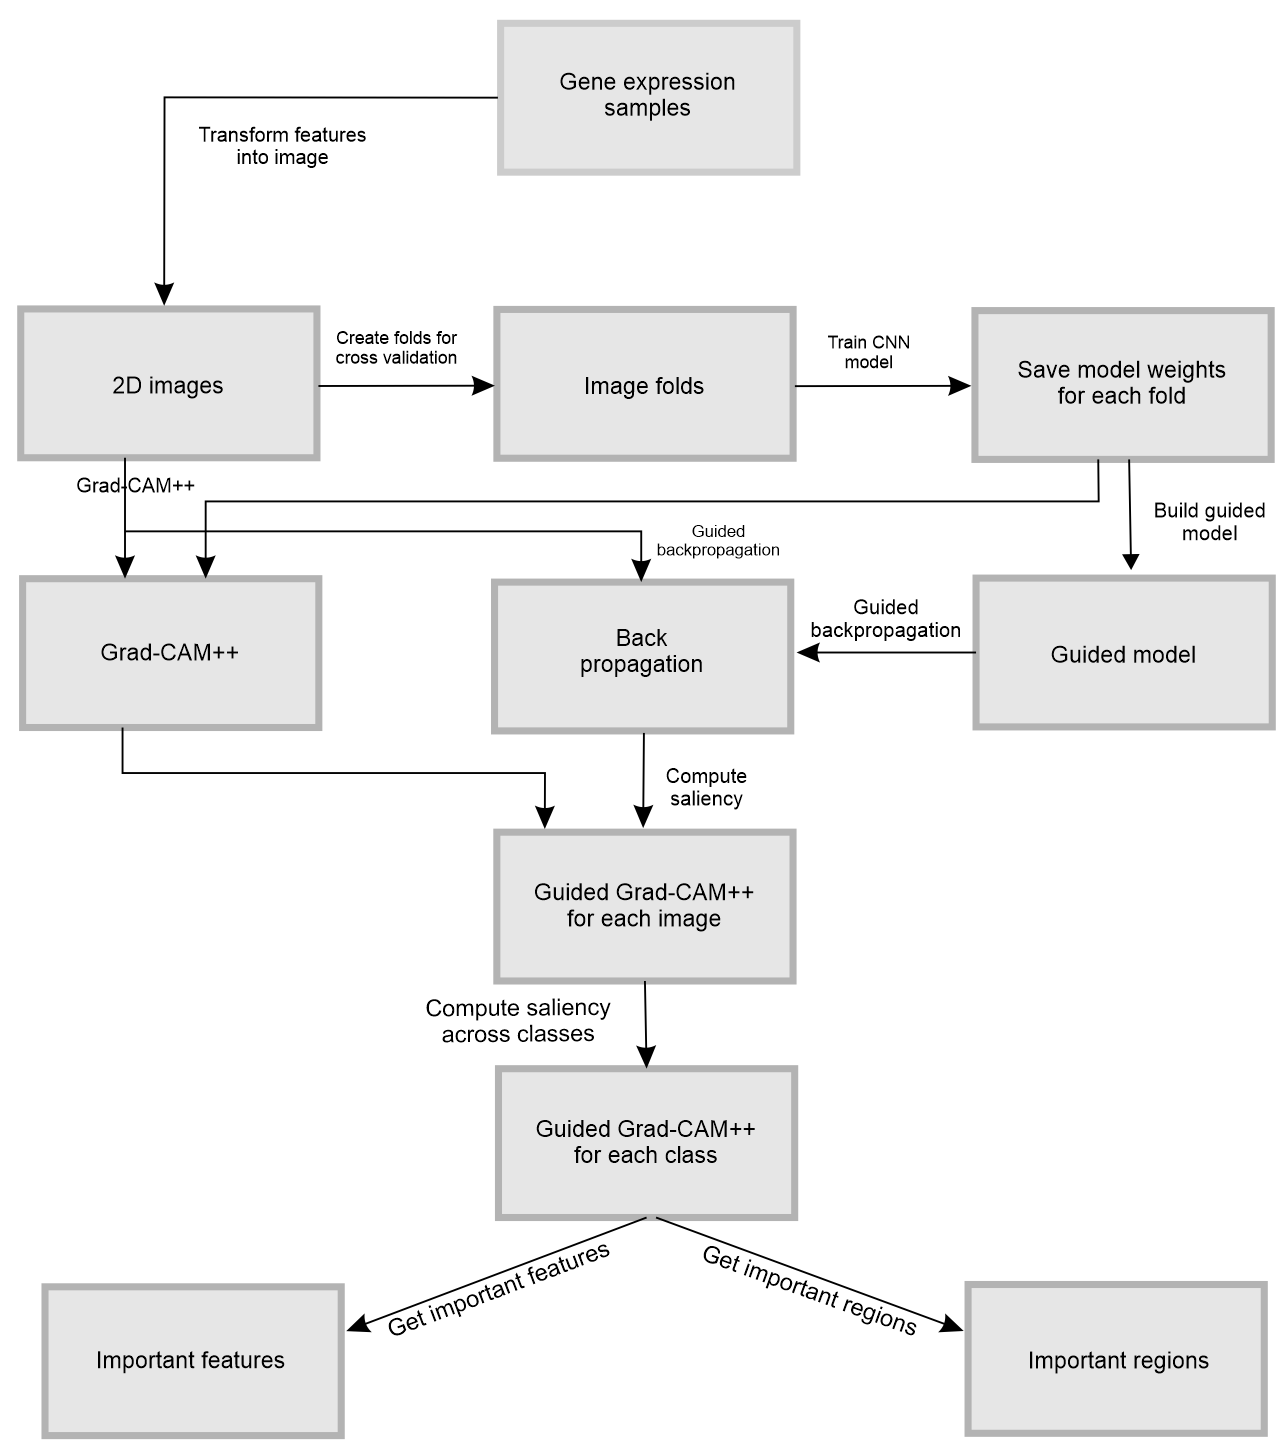
\includegraphics[scale=0.9]{images/wf_2D_CNN.png}
    \caption{Workflow of the unimodal CNN modality approach}	
	\label{fig:workflow_2D_CNN}
\end{sidewaysfigure*}

%\subsubsection{Preprocessing}
%The pooling layer is calculated by down-sampling the convolutional layer by taking the maximum value in each non-overlapping sub-region.

\subsubsection{Network construction and training}
In order to find the relation between instances, e.g., GE of a particular cohort in relation to other types tumors,  mean normalization per gene is performed for each modality data. Second, samples are embedded as 2D images\footnote{To perform 2D convolutional operations with ease} in which respective expression values. Each sample is reshaped from a 20,501$\times$1 array into a 144$\times$144 image by adding zero padding around the edges and normalized to [0,255].%, without losing any information.
As shown in \cref{fig:clstm2}, both vanilla CNN and VGG16 architectures are constructed and trained from scratch, in a similar fashion. In either network training, output of a convolutional layer is first passed through a dropout layer to avoid possible overfitting~\cite{vardropout}. To down sample the output~(lower-level feature space) of a convolutional layer into lower dimensional representation, two max pooling layers~(MPL) are placed, by setting different filter size. Output of an MPL can be considered as `extracted features' from 2D image samples. Since an MPL flattens the output space by taking the highest value in each convolutional feature map, more abstract features are learned by the last MPL. This can be thought as the feature selection process for finding highly indicative driver genes responsible for specific cancer types.

\begin{figure*}[h]
	\centering
	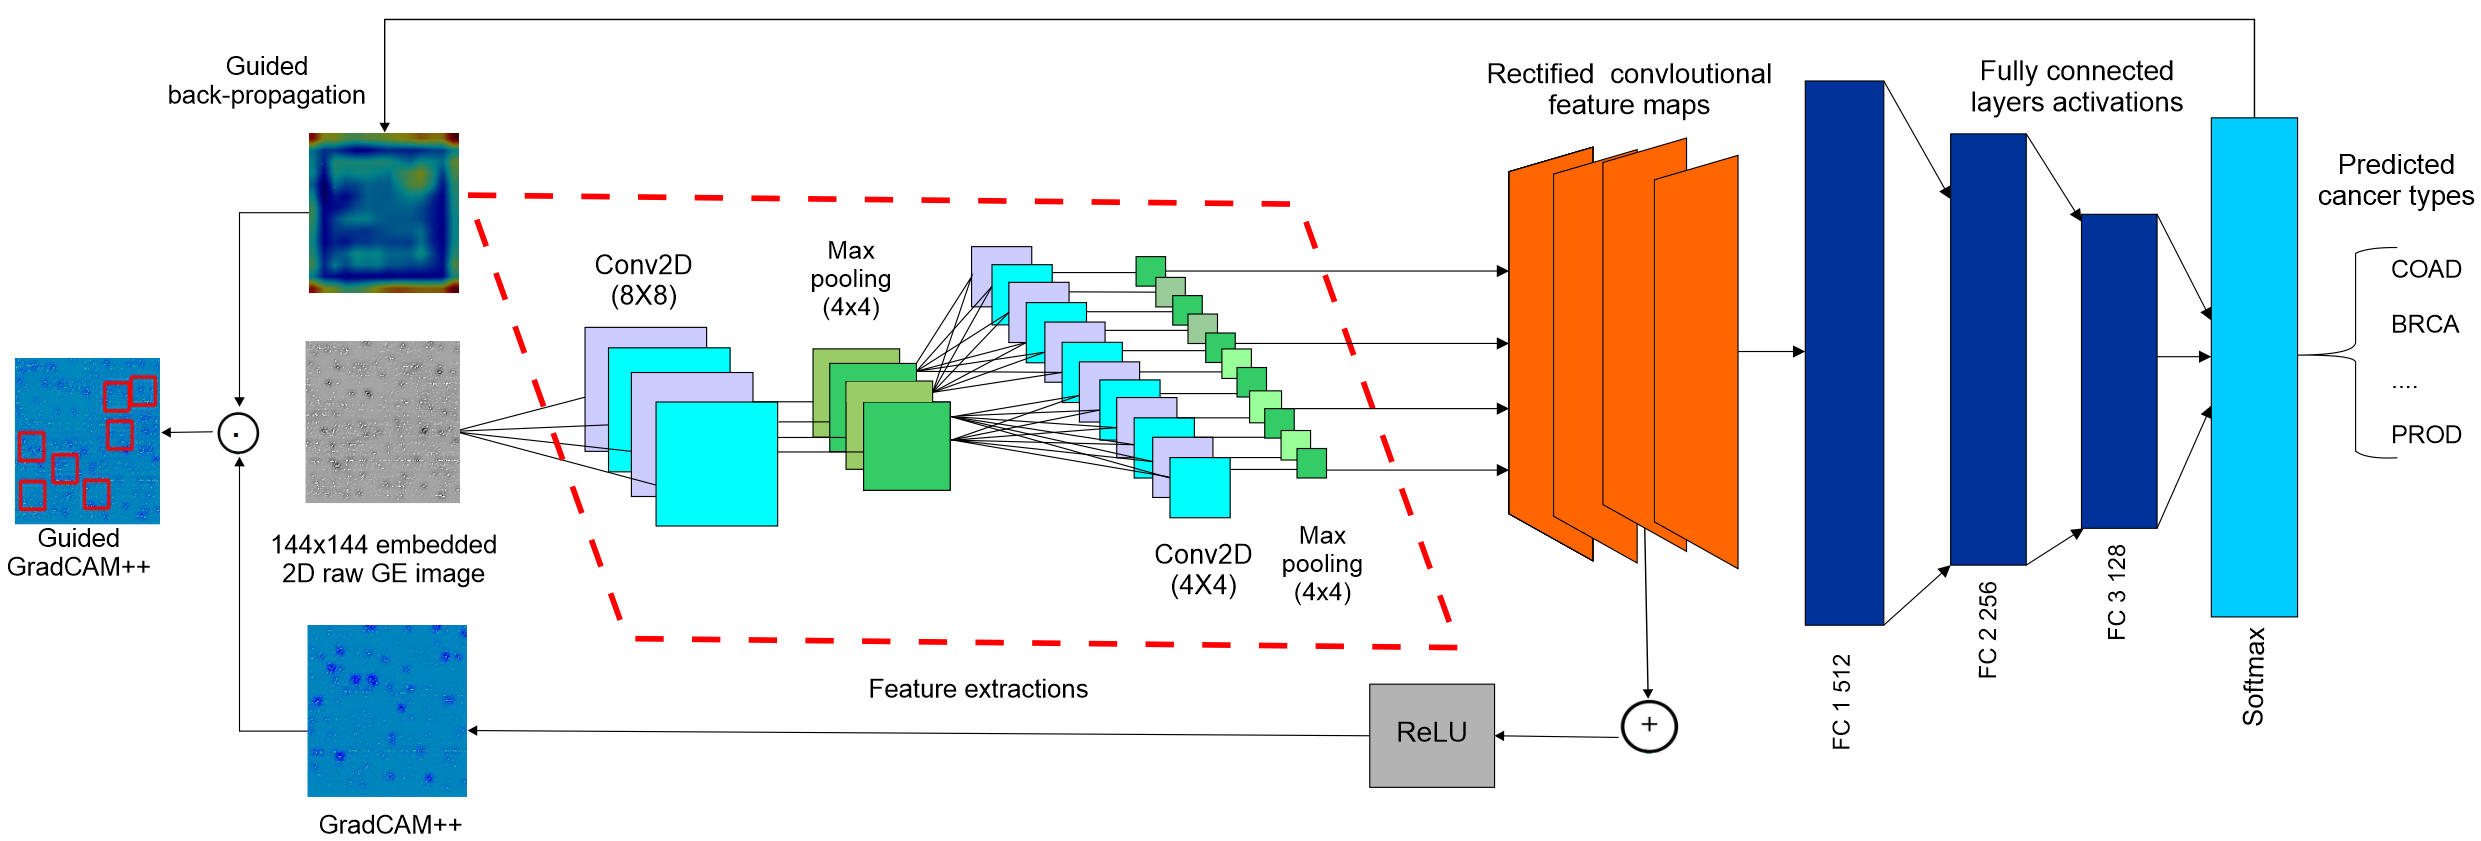
\includegraphics[scale=0.5]{images/clstm.PNG}
    \caption[Schematic representation of CNN-based approach]{Schematic representation of CNN-based approach, which starts by taking a raw GE sample as input and passing it through convolutional and pooling layers to generate rectified convolutional feature maps. Feature maps are then passed through fully connected softmax layer for classification. Guided back-propagation and Grad-CAM++ are applied to identify important important genes w.r.t pixel values.}	
	\label{fig:clstm2}
\end{figure*}

\hspace*{3.5mm} Finally, 2D feature maps from MPL are flattened and transform into feature vector, which is fed into a fully connected softmax layer~(FCL). A FCL consist of 3 dense, a dropout, and a softmax layers. It is to be noted that weights for none of these networks were not initialized from any pretrained models. The reason is that deep CNN architectures are usually trained from ImageNet, which contains photos of general objects. Subsequently, internal representation of network's hidden layers will be activated with geometrical forms, colorful patterns, or irrelevant shapes that are usually not present in genomics datasets. Both vanilla CNN and the VGG16 architectures are trained with gradient-based AdaGrad optimizer, which optimizes the following categorical cross-entropy~(CE) loss: 

\begin{equation} 
    L_{ce}=-\sum_{m=1}^{C} y_{k} \log \left(\hat{y}_{k}\right) \label{eq:ce_loss_function},
\end{equation} 

\hspace*{3.5mm} where $m \in \mathbb{R}^{C}$ is the number of classes, $y_{k}$ is the ground-truths for modality $k$ and $\hat{y}_{k}$ is the predicted output. The softmax activation function, which is used in the output layer transforms output of the last dense layer into a vector of real number within the range of $\left(0,1\right)$. This can be considered as probabilistic interpretation, i.e., probability distribution over the classes, before computing the CE loss. Further, effects of adding Gaussian noise layers is observed, with the objective improving model generalization for unseen test data. Gaussian noise is a natural choice as corruption process for real valued inputs, which makes it suitable to introduce noise to input values or between hidden layers. 

%Since an appropriate selection of hyperparameters can have a huge impact on the performance of a deep architecture, we perform the hyperparameter optimization through random search and 5-fold cross-validation tests. 

\subsubsection{Probing black-box CNN models}
Data for each modality is high dimensional, where majority of features~(genes) are not responsible for cancer, making them irrelevant for the cancer type classification. Therefore, it is more reasonable to probe both CNN and VGG16 networks to leverage the biomarker identification~(most important features). \Cref{algo:hm} and \ref{algo:imp_area} depict the pseudo-codes for computing feature importance with ranking genes and identification of important areas on the HM, respectively. Inspired by the Grad-CAM based probing technique by Selvaraju et al.~\cite{mostavi2019convolutional}, all the normalized HMs from the same class are averaged to generate a class-specific HM. However, since Grad-CAM++ requires all the samples to run through the network once, activation maps are set and recorded in the forward pass. 

\hspace*{3.5mm} On the other hand, to collect the HM for each sample, gradient maps are generated in the backward pass, i.e., during the back-propagation. A higher intensity pixel in a HM signifies higher importance of corresponding gene and it's value to the final prediction. Top genes are then selected based on the intensity rankings and MAI threshold. However, since SM use true gradients, trained weights are likely to impose a stronger bias towards specific subsets of the input pixels. Therefore, LRP was applied on both CNN and VGG16 trained CNN models to generate heatmaps for each sample in the test set.A heatmap highlights class-discriminating features~(on 2D pixel space) showing relevance for diagnosis decisions. 

\begin{algorithm*}[h]
\small
    \DontPrintSemicolon \SetKwInOut{Input}{Input}%
      \SetKwInOut{Output}{Output}%
      \Input{2D images ${X_k}=(d_1,d_2,\dots,d_n)$ for $k$ input modality, labels ${L}=(l_1,l_2,\dots,l_n)$ on which a CNN model is trained for each fold ${M}=(m_1,m_2,\dots,m_i)$.}%
      \Output{feature importance ${F}=(f_1,i_1),\dots,(f_n, i_n)$, top features ${T}$ for all images per fold per class.}%
      \BlankLine%
     \For{$\mathit{m} \in \mathit{M}$}{
       ${P} \leftarrow  \{\}$ \tcp*{Guided backprop for each image per fold per class}\; 
      \vspace{-4mm} 
       ${K} \leftarrow  \{\}$ \tcp*{Grad-CAM++(GCAM) for all images per fold per class}\; 
      \vspace{-4mm} 
       ${I} \leftarrow  \{\}$ \tcp*{GCAM of each image in a fold}\; 
      \vspace{-4mm} 
      ${G} \leftarrow  \{\}$ \tcp*{GCAM for all images per fold per class}\; 
      \vspace{-4mm} 
      ${F} \leftarrow  \{\}$ \tcp*{Feature importance of each gene per class per fold}\; 
      \vspace{-4mm} 
      ${T} \leftarrow  \{\}$ \tcp*{Top genes and importance per class per fold}\; 
      	\vspace{-4mm} 
      	\For {$d \in {X_k}$}{ 
    		${K} \leftarrow \mathit{gradCAM++}(m, d, l)$ \tcp*{GCAM of an image per fold per class}\;
    		\vspace{-4mm} 
    		${P} \leftarrow \mathit{guidedBackprop}(m, d)$ \tcp*{Guided backprop of an image}\;
    		\vspace{-4mm} 
    		${I} \leftarrow {K} * {P}$ \tcp*{GCAM for an image}\;
    		\vspace{-4mm} 
    		${G} \leftarrow {G}\cup {I}$ \tcp*{GCAM for all the images in a fold}\;
    		\vspace{-4mm} 
    	    } 
    	${F} \leftarrow \frac{1}{M}\sum_{i=1}^M {G_i}$ \tcp*{Mean absolute impact for genes for axis=0}\;
    	\vspace{-4mm} 
    	\If{$F_i < \sigma $}{ \tcp*{If the feature importance is less than MAI}\;
    	\vspace{-4mm} 
        	${F} \leftarrow  F - F_i$ \tcp*{Pop off insignificant genes}\;
        	\vspace{-4mm} 
        	${T} \leftarrow  \operatorname{sort}_k(F)$ \tcp*{Sort and choose top genes based on MAI}\;
        	\vspace{-4mm} 
    	}
    	\textbf{Return} ${F}, {T}$
     }
    \caption{Computing feature importance and ranking genes}
     \label{algo:hm}
\end{algorithm*}

\begin{algorithm*}
\small
    \DontPrintSemicolon \SetKwInOut{Input}{Input}%
      \SetKwInOut{Output}{Output}%
      \Input{importance of current class across folds ${F}=(f_1,\dots,f_i)$, height $h$ and width $w$ of rectangle, and MAI threshold $\sigma$.}%
      \Output{important areas ${C} = (x_{1}, y_{1}),(x_{2}, y_{2}),\dots,(x_{n}, y_{n})$ in an image per fold.}%
      \BlankLine%
     \For{$\mathit{m} \in \mathit{M}$}{
      ${A} \leftarrow \mathit{dict}()$ \tcp*{Importance of areas}\; 
      \vspace{-4mm} 
      ${S} \leftarrow \mathit{list}()$ \tcp*{Sorted areas by MAI}\; 
      \vspace{-4mm} 
      ${C} \leftarrow \mathit{list}()$ \tcp*{Important areas}\; 
      \vspace{-4mm} 
      \For {$h$}{ 
        	\For {$w$}{ 
    		$area \leftarrow {F}[h:h + \mathit{shape}[0], w:w + \mathit{shape}[1]]$ \tcp*{Area of image}\;
    		\vspace{-4mm} 
    		$impA \leftarrow 0$\tcp*{Importance of current area in the image}\;
    		\vspace{-4mm} 
    		\For {$\mathit{row} \in \mathit{area}$}{
    		%\vspace{-4mm} 
    			\For {$\mathit{imp} \in \mathit{row}$}{
    			%\vspace{-4mm} 
    			\If{$\mathit{imp} > \sigma$}{ \tcp*{If feature importance is greater than MAI}\;
    			\vspace{-4mm} 
    			    $\mathit{impA} += \mathit{imp} - \sigma$ \tcp*{Importance of area = current importance - MAI}\;
    			    \vspace{-4mm}
    			    }
    			  }
    		}
            ${A}[\mathit{area}] = \mathit{impA}$ \tcp*{We update the importance of the area}
    	     } 
    	    }
    	${S} \leftarrow \operatorname{sort}({A}, \mathit{reverse}=\mathit{true})$ \;
    	\For {$a, i \in {S}$}{
    	\If{$a \cap i = \empty$}{ \tcp*{Non-intersecting area with important areas}\;
    		\vspace{-4mm} 
        	${C} \leftarrow {C}  \cup a$ \tcp*{It's a new important area added to the list}\;
        		\vspace{-4mm} 
    	}}
    	\textbf{Return} ${C}$
     }
     \caption{Identification of important areas}
     \label{algo:imp_area}
\end{algorithm*}

 %The idea is also to find the most important biomarkers by ranking them based on MAI threshold. 
%\hspace*{3.5mm} 

\begin{figure*}[h]
	\centering
	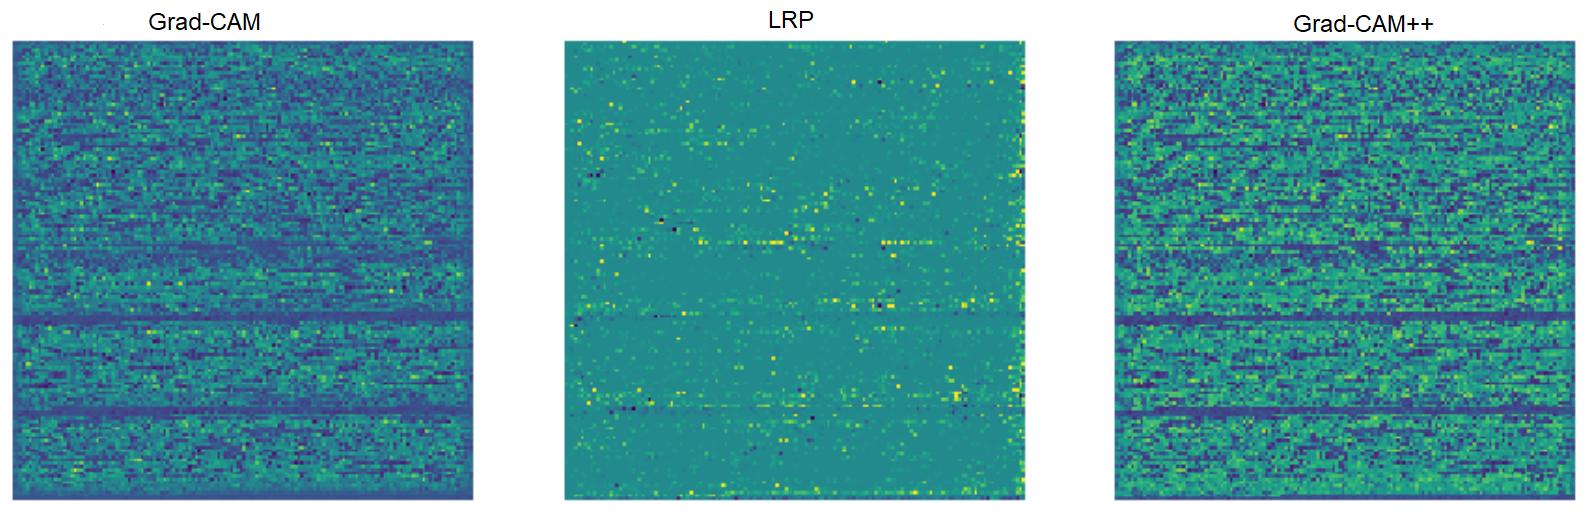
\includegraphics[scale=0.7]{images/3_mode.png}
	\caption[Heat map examples for a single cancer type prediction]{Heat map examples for a single cancer type prediction, where the image-pixel of specific biomarkers are highlighted by probing the network with Grad-CAM, Grad-CAM++, and LRP.} 
	\label{fig:3hms}
\end{figure*}

\hspace*{3.5mm} To observe if the feature identified by CNNs are statistically significant and comparable to established feature ranking approaches such as random forest-based estimates, we compute feature importance for the driver genes. The permutation feature importance is computed on top of a trained model $f$. For each feature $x_i$ in dataset $X_k$ and for each repetition $r$ in $1, 2, \ldots, R$, column $x_i$ is randomly shuffled to generate a corrupted version of the data $\tilde{X_k}_{r,x_i}$. Then a reference balanced score~(F1-score in our case) $s_{r,x_i}$ is computed for $f$. Subsequently, the mean importance $\sigma_{x_i}$ for feature $x_{i}$ is computed as follows: 

\begin{align}
    \sigma_{x_i}=s-\frac{1}{R} \sum_{r=1}^{R} s_{r,x_i}.
\end{align}

\iffalse
Using ELI5, permutation feature importance are computed on top of the trained model $f_k$. For the dataset $X_k$, the reference `accuracy' score $Acc$ is computed. For each feature $x_i$ and for each repetition $p$ in $1, 2, \ldots, P$, column $i$ is randomly shuffled to generate a corrupted version of the data $\tilde{X}_{p,i}$. Score $Acc_{p,i}$ is then computed, followed by the calculation of mean importance $I_{i}$ of $x_{i}$, as follows~\cite{SHAP}:

\vspace{-2mm}
\begin{align}
    I_{i}=s-\frac{1}{P} \sum_{p=1}^{P} s_{p,i}
\end{align}
\fi 

\hspace*{3.5mm} Although permutation feature importance provides a view on global feature importance and signifies how important a feature is for a particular model, it does not necessarily reflect the intrinsic predictive value of a feature by itself~\cite{molnar2019interpretable}. There is a possibility that a feature that seems to have lower importance for a under/overfitted model could be very important for a better fitted model. Nevertheless, the order in which a model sees features can affect the predictions. In SHapley Additive exPlanations~(aka. SHAP)~\cite{SHAP} interpretable method, feature importance is an alternative to the permutation feature importance discussed above. The only difference is how the importance is measured. Permutation feature importance is based on the decrease in model performance, while SHAP is based on magnitude of feature attributions~\cite{molnar2019interpretable}. 

\hspace*{3.5mm} The goal is to explain the prediction of sample $x_i$ by computing the contribution of each feature in the prediction w.r.t Shapley values. Shapley values that are based on coalitional game theory~\cite{branzei2008models}\footnote{In game theory, a cooperative game played with competition between groups of players known as ``coalitions'' as there is a possibility of external enforcement of cooperative behavior. The cooperative game theory focuses on predicting which coalitions will form, the joint actions that groups take and the resulting collective payoffs.} is used as the measure of feature attributions. Feature values of $x_i$ act as players in a coalition such that the Shapley values tell us how to fairly distribute the  payout~\cite{molnar2019interpretable}. This can be correlated with distributing the prediction contributions among the features in a sample. SHAP specifies the explanation as follows~\cite{molnar2019interpretable}:

\begin{equation}
    f\left(z^{\prime}\right)=\phi_{0}+\sum_{j=1}^{M} \phi_{j} z_{j}^{\prime},
\end{equation}

\hspace*{3.5mm} where $f$ is an explanation model, $z^{\prime} \in\{0,1\}^{M}$ is the coalition vector\footnote{Less technically, coalition vector is simplified feature representation for tabular data}, $\mathrm{M}$ is the maximum coalition size, and $\phi_{j} \in \mathbb{R}$ is the feature attribution for a feature $\mathrm{j}$ or Shapley values. The computation is repeated in all possible orders to compare the features fairly. If $x_i$ is a feature in modality specific input $X_k$, it's importance w.r.t Shapley value $\phi$ is computed by comparing what the model predicts with and without $x_i$ for all possible combinations of $n$ features in $X_k$. For $x_i$, prediction $\hat x_i$ and $\phi$ are then calculated as~\cite{NIPS2017_7062}. 

\vspace{-2mm}
\begin{align}
    \phi_{i}(\hat x_i)=\sum_{X_k \subseteq N / i} \frac{|X_k| !(n-|X_k|-1) !}{n !}(\hat x_i(X_k \cup i)-\hat x_i(X_k)).
    \label{eq:shap}
\end{align}

\hspace*{3.5mm} If $x_i$ has no or almost zero effect on the predicted value, it is expected to produce a Shapley value of 0. If two features $x_i$ $x_{i+1}$ contribute equally to the prediction, Shapley values should be the same~\cite{NIPS2017_7062}. In SHAP, features with large absolute Shapley values are more important than others. In order to compute global importance, absolute Shapley values per feature~(across the data) are averaged as~\cite{NIPS2017_7062}:

\begin{equation}
    I_{j}=\sum_{i=1}^{n}\left|\phi_{j}^{(i)}\right|.
\end{equation}

\hspace*{3.5mm} Although feature importance is used to provide global explanations by highlighting important features, plot only the value per feature is often not very insightful. Therefore, using the Shapely values, summary plot is more widely used, where feature importance is combined with feature effects. More detail will be discussed in a later chapter. It is to be noted that both CNN and VGG16 trained models are evaluated on a held-out set prior computing the feature importance using permutation feature importance and SHAP.

\subsection{Constructions and training of multimodal classifiers}
The multimodality nature of the data motivated us to develop MAE deep architecture. MAE was based on vanilla AE, where the concept of shared latent representation~(SLR)~(see \cref{fig:slr_11}) is used to generate the shared feature representation of the multimodal input. MAE moderately performed for breast cancer subtype classification tasks, which is largely due to high pretraining and reconstruction losses.
In a recent approach proposed by Patrick T. et al.~\cite{mmdcae}, another multimodal concept learning called latent representation concatenation~(LRC)~(see \cref{fig:lrc_11}) is proposed. Base on several studies, covering text classification, sequence data, and imaging, they identified the following potential limitations of SLR: 

\begin{itemize}[noitemsep]
    \item The reconstruction loss for LRC is significantly lower compared to SLR.
    \item When a classifier is trained on features learned by LRC, accuracy improves significantly, which is largely backed by lower reconstruction loss. 
\end{itemize}

\hspace*{3.5mm} Inspired by the success of LRC and considering the limitations of MAE and SLR, multimodal convolutional autoencoder classifier~(MCAE) is constructed to improve the classification accuracy. As shown in \cref{fig:lrc_11}, MCAE is based on convolutional autoencoder~(CAE) and LRC-based representation learning. Besides, to show the effectiveness of MCAE and LRC, another variant of MCAE classifier is trained on SLR-based latent representation, as shown in \cref{fig:slr_11}. 

\begin{sidewaysfigure*}[htp!]
	\centering
	\begin{subfigure}{.48\linewidth}
		\centering
		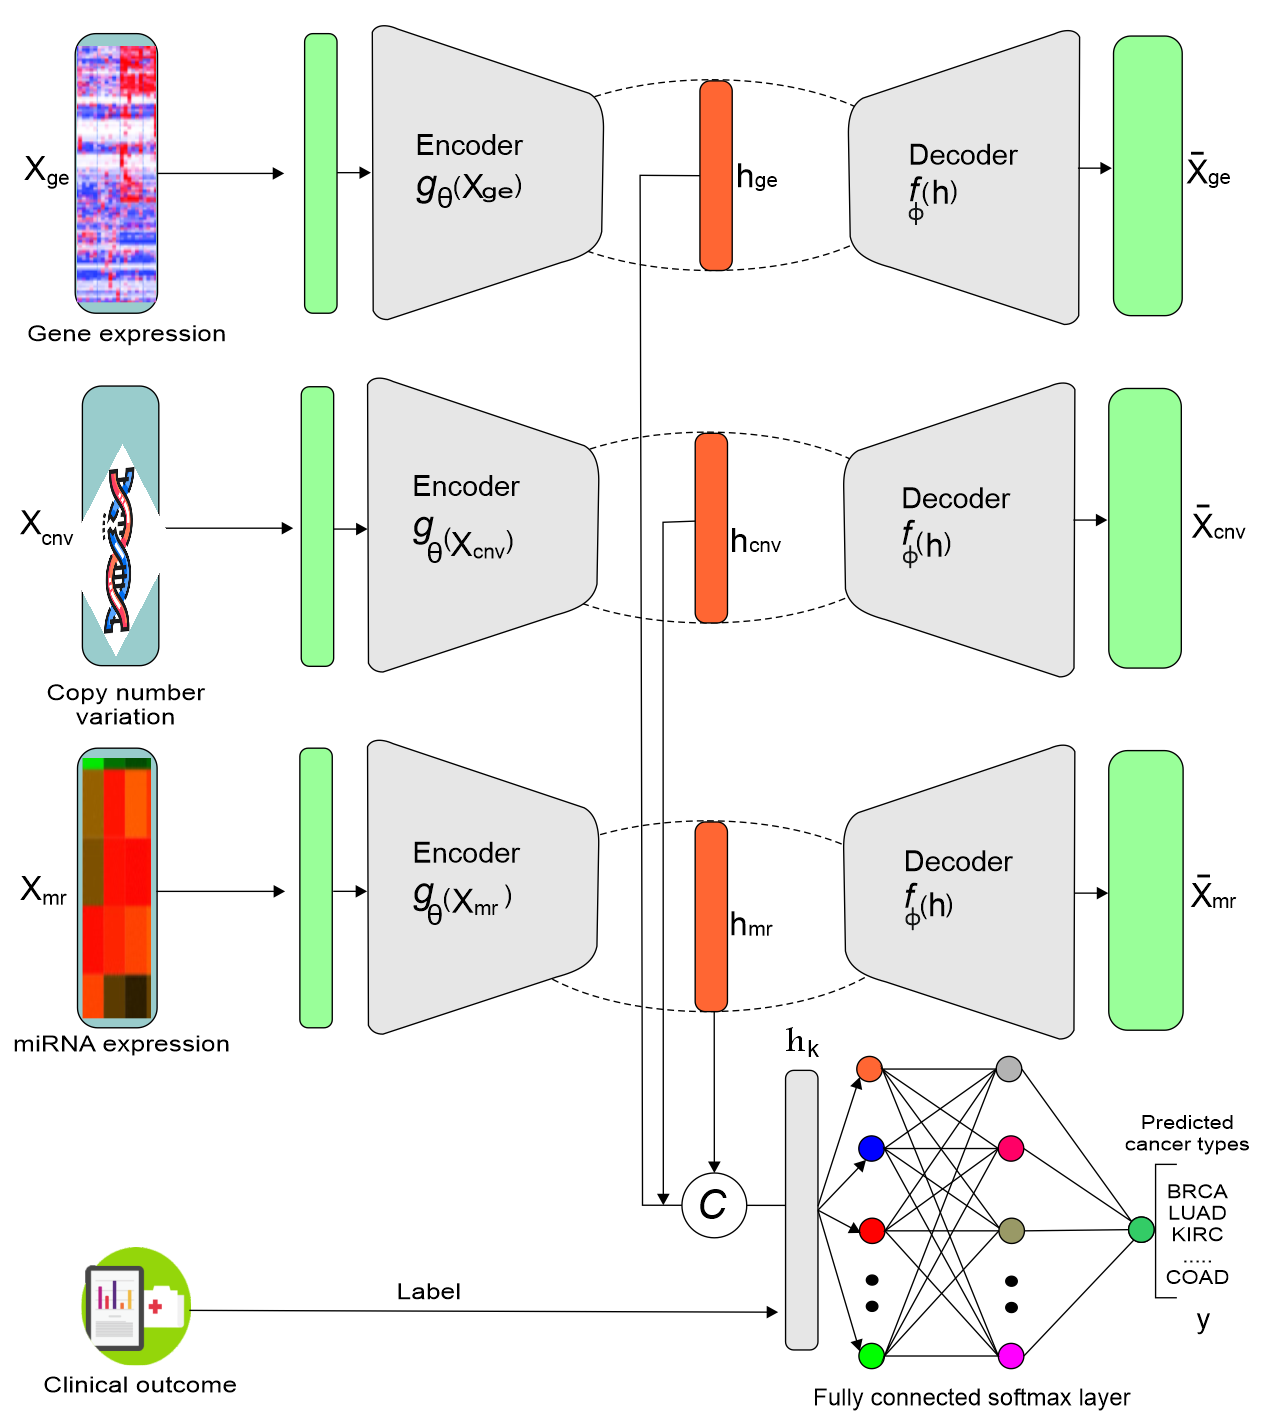
\includegraphics[scale=0.7]{images/lrc_rl_mcae.png}
		\caption{Representation learning based on LRC and classification}
        \label{fig:lrc_11}
	\end{subfigure}
	\begin{subfigure}{0.48\linewidth}
		\centering
		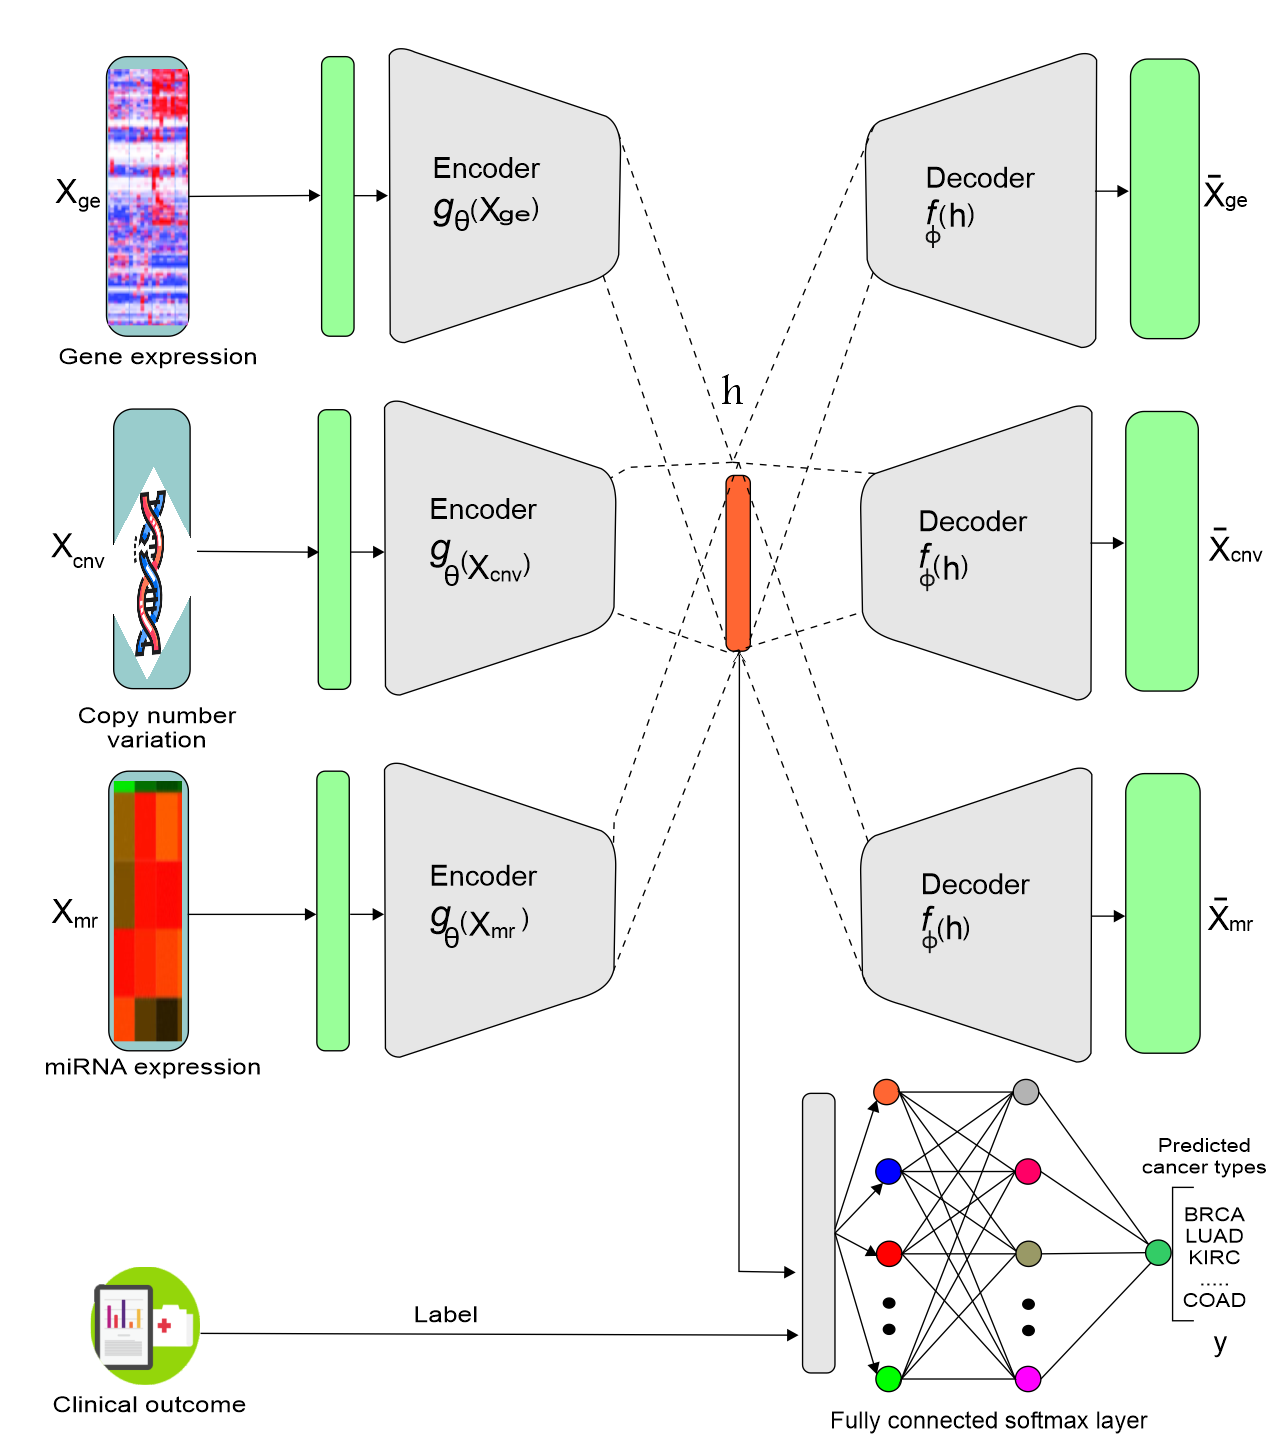
\includegraphics[scale=0.7]{images/clr_rl_mcae.png}
		\caption{Representation learning based on SLR and classification}
        \label{fig:slr_11}
	\end{subfigure}
	\caption{Fusion architectures in multimodal representation learning and classification} 
	\label{fig:mm_rL_example1}
\end{sidewaysfigure*}

\iffalse
\subsubsection{Construction of MCAE}
Although a single and simple AE discussed in \cref{preli:AEs} can reconstruct an output similar to the original input, it cannot handle multimodality. Nevertheless, traditional supervised learning is only able to learn from the intersection of samples, which are both clean and labeled. In contrast, weights of the MCAE encoder learn from both unlabelled data, and noisy supervised data with missing modalities, leveraging as much of the available data as possible. Architecturally, MCAE is similar to a three-stage CAE: the first stage represents a particular modality for each type of data, and the second stage represents the cross-modality. CAE is trained to find a low-dimensional representation of the multimodal data, taking advantage of the information that one modality provides about another. 

\iffalse
\begin{figure*}[htp!]
	\centering
	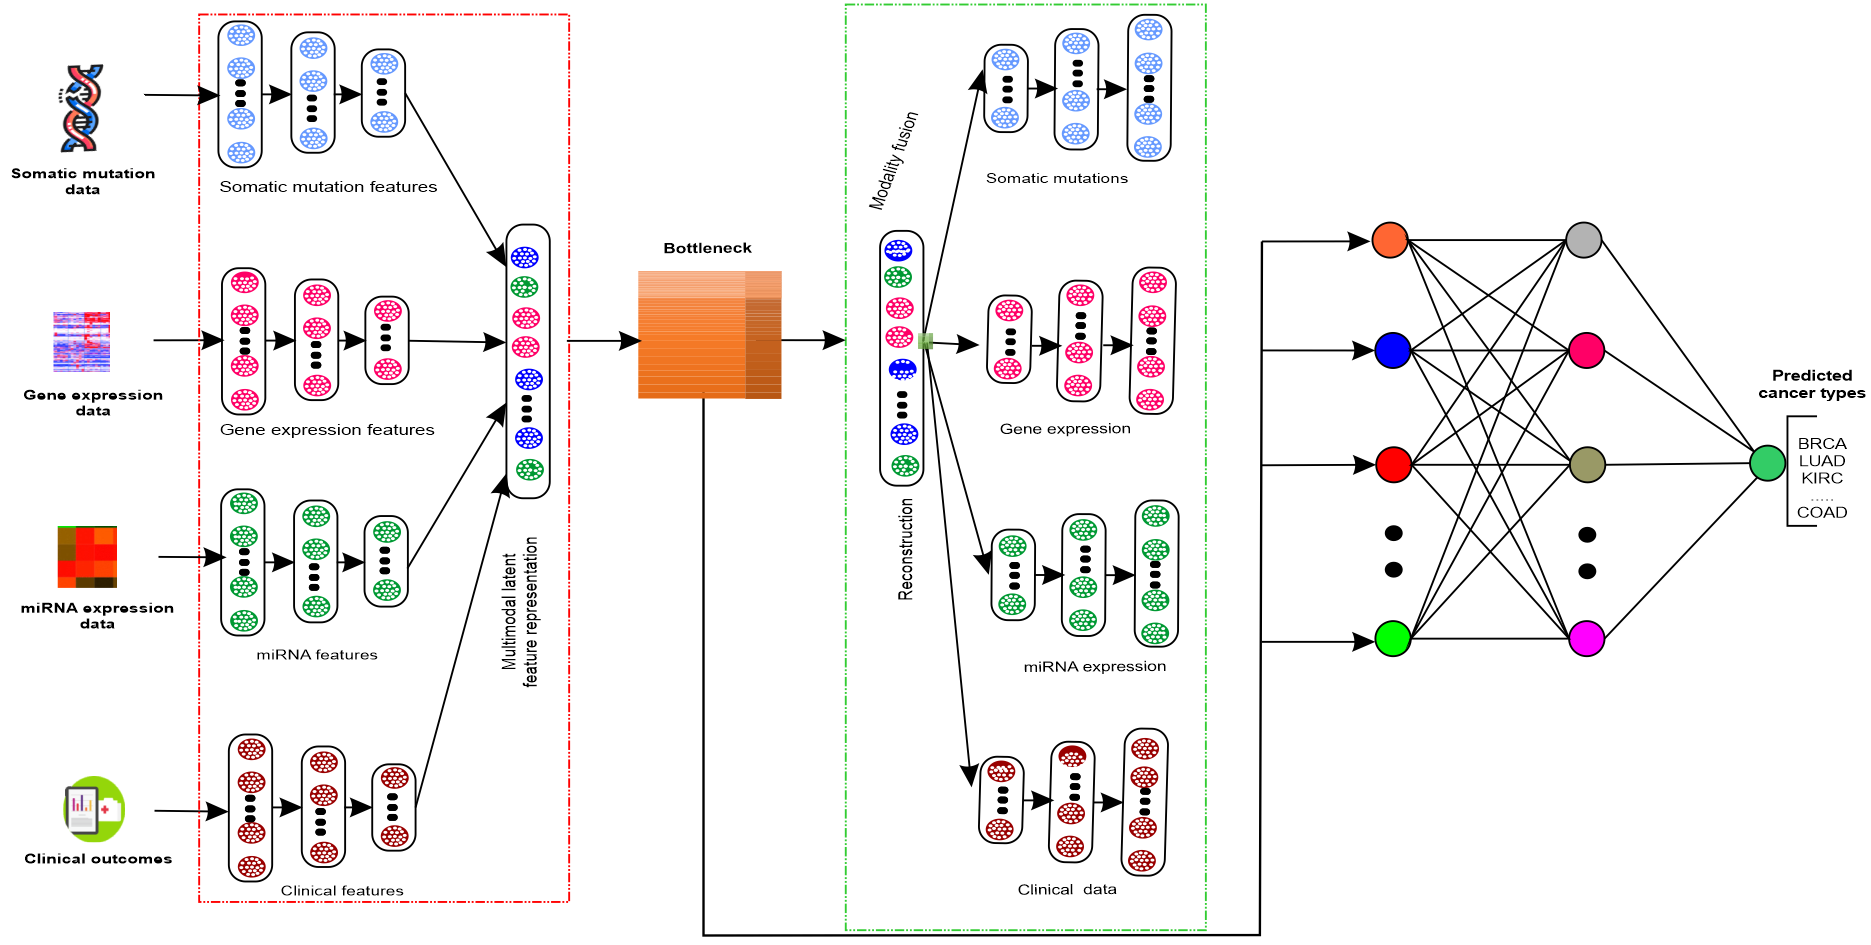
\includegraphics[width=\textwidth]{images/mcae.png}	
    \scriptsize{\caption{schematic representation of the cancer typing method based on multimodal convolutional autoencoder, which starts from taking GE, miRNA, mutations, and clinical outcomes and passing to convolutional layers before obtaining rectified conv feature maps~(with guided-backprop and GradCAM++) to pass through dense, dropout, and softmax layer}}.	
	\label{fig:mcae}
\end{figure*}
\fi 

\hspace*{3.5mm} We illustrate the construction of an MCAE as a quad-modal AE, where CNV, GE, miRNA expression, and clinical outcomes form 4 different modalities from the same patient cohorts. The individual modality CAE is not only a one-layer AE, but a multilayer and gradually shrinking CAE with the possibilities of a different number of layers for each modality, which is due to difference in dimension between modalities are pretty large. By default, MCAE fuses multiple modalities consists of a variable number of ReLU layers, which are densely connected. The cross-modality CAE is also a multilayer gradually shrinking CAE with different output layer for each prediction. However, number of layers and units per layer of the encoder and decoder networks are symmetric. The $3^{rd}$ stage is the supervised MCAE in which the decoder part is removed, and only the encoder part is utilized by adding a fully connected layer for the classification. % and regression operations. 
\fi 

\subsection{Training of MCAE}
A single and simple AE can be used to reconstruct an output similar to the original input. However, it cannot handle multimodality~(i.e., different types of information). Weights of a encoder module is learned from both non-corrupted and unlabeled data. Subsequently, noisy supervised data with missing modalities is not suitable for learning latent features. Nevertheless, the difference among input modalities are pretty large in terms of the dimensionality. For example, sometimes GE data come with about 20,000 features, but miRNA data has only 5,000 features. Non-trivial challenge in modality specific representation learning and limitations of MAE architecture are enough motivations to employ multimodal representation learning and classification based on multimodal CAE architecture~(MCAE). 

\hspace*{3.5mm} Although CNNs are known as effective feature extractors, instead of using manually engineered convolutional filters in CNN, convolutional and pooling layers can be stacked together to construct a stacked convolutional autoencoder~(CAE), to leverage better feature extraction capability~\cite{alirezaie2019semantic}. This makes CAE, compared to vanilla AE based multimodal learning, more effective for very high dimensional data. In particular, CAE learns more optimal filters by minimizing the reconstruction loss, which results in more abstract features from the encoder~(e.g., pixel-level features from images, when genomic samples are embedded into 2D pixel-space~\cite{mostavi2019convolutional}). This helps to stabilize the pretraining. Subsequently, the network converges faster by avoid corruption in feature space~\cite{guo2017deep}. 

\hspace*{3.5mm} Since individual latent representation is require to have the same dimensionality~\cite{mmdcae}, MCAE architecture depicted in \cref{fig:slr_1} is used to generate a combined representation for all input modalities, instead of one latent representation for each input modality. From the network topological point of view, MCAE creates hierarchical hidden units by stacking multiple CAEs, which have a strong connection between nodes not only for individual modality, but also across the modalities. Training MCAE involves pre-training to leverage the representation learning, followed by supervised fine-tuning on learned representation. 

\subsubsection{Unsupervised pertaining of MCAE} 
Pre-training is similar to training a two-stage CAE network: the first stage represents modality specific learning. The second stage corresponds to cross-modality. Pre-training is performed greedily on each layer of the network, which corresponds to representation learning with individual CAEs. 

\paragraph{Stage-1: individual modality}\hspace{-3mm} of MCAE represents a specific modality for each type of data. Individual modality CAE is not only a one-layer CAE, but also a multilayer and gradually shrinking CAE with different number of layers per modality. An CAE consist of two sub-networks called encoder and decoder. Each layer of CAE consists of an encoder, that performs convolution and pooling, and a decoder that performs unpooling and deconvolution operations. More technically, an encoder is a sigmoid function $g(.)$ parameterized by $\phi$~(refer to below for detail), while the decoder function $f(.)$ is parameterized by $\theta$. %~(refer to below for detail). 

\hspace*{3.5mm} Assuming input $X_{k} \in \mathbb{R}^{D}$ for each of $k \in \mathbb{R}^K$ modalities is consisting of $n$ samples, a convolutional layer first calculates the convolutional feature map. Max-pooling operation is then performed, which downsamples the output of the convolutional layer by taking the maximum value in each non-overlapping sub-region. Thus, $X_{k}$ is mapped and transformed into a lower-dimensional embedding space, $Z_k$. Assuming, $p$ and $p$ are number of input and hidden units, respectively, latent-space representation $Z_k=g_{\phi}(X_{k})$ is learned in the bottleneck layer~\cite{mmdcae}: 

\begin{equation}
    Z_k = h_{k}=g_\phi \left({X}_{k}\right)=\sigma\left(W_{k} \oslash X_{k}+b_{k}\right),
    \label{eq:fcuk_1}
\end{equation}

\hspace*{3.5mm} The final feature maps $Z_k$ are latent variables, specific to modality $k$. In \cref{eq:fcuk_1}, where $\phi$ are trainable parameters~(which include a weight matrix $W_{k} \in \mathbb{R}^{p \times q}$ and a bias vector $b_{k} \in \mathbb{R}^{q}$ that are specific to respective modality $k$), $\oslash$ is the convolutional operation, and $\sigma$ is the ELU~\cite{clevert2015fast} activation function\footnote{Unlike MAE architecture, where ReLU activation function was used.}. Then the decoder module reconstructs from $h_k$, the original input $X_{k}$ from the latent representation $Z_k$ using the decoder function $f(.)$. Hidden representation $h_{k}$ is mapped back as reconstructed version $\hat{X}_{k}$, similar to original input ${X}_{k}$, as follows~\cite{mmdcae}: 

\begin{equation}
    \hat{X_k}=f_{\theta}\left(Z_k\right)=f_{\theta}\left(g_{\phi}({X_k})\right) \label{eq:mcae_eq_1},
\end{equation}

\hspace*{3.5mm} where parameters $(\theta,\phi)$ are jointly learned to output a reconstructed version of the original input. This is analogous to learn an identity function, such that $\hat{X_k} \approx f_{\theta}\left(g_{\phi}({X_k})\right)$, i.e., $f_{\theta}\left(g_{\phi}({X_k})\right)$ is equivalent to $\Psi \left(\hat W_k * h_k + \hat b_{k}\right)$. Therefore,  \cref{eq:mcae_eq_1} is changed to following form: 

\begin{equation}
    \hat{X_k}=\Psi \left(\hat W_k \odot h_k + \hat b_{k}\right),
\end{equation}

\hspace*{3.5mm} where $\odot$ is the de-convolutional operation, $\theta$ are trainable parameters~i.e., weight matrix $\hat W_{k} \in \mathbb{R}^{n \times p}$ and bias vector $\hat b_{k}$) specific to modality $k$, and $\Psi$ is sigmoid activation function. The decoder module has a similar gradual increasing architecture as an encoder, where both unpooling and deconvolution operations are performed. The unpooling is performed with switch variables such that it remembers the position of the maximum value during the max-pooling operation. More technically, within each neighborhood of $Z_k$, both the value and location of the maximum element are recorded: pooled maps store the values, while switches record the locations. Distance measure~($d_{k}$) that quantifies difference between input $X_{k}$ and network's output $f_\theta(X_{k})$, is used as a typical reconstruction loss, assuming $X_k$ consists of $n$ samples~\cite{KarimIEEEAccess2019}: 

\begin{equation}
    L_{\mathrm{k}}(\theta, \phi)=\text{$d_{k}$}(X_{k}, f(X_{k}) = \sum_{i=1}^{n} \left\|X_{k}-f(X_{k})\right\|^{2}.
    %\label{eq:Loss1}
\end{equation}

\hspace*{3.5mm} Above loss is iteratively optimized. Replacing $f(X_{k})$ with $\hat{X}_{k}$, above equation is changed to: 

\begin{equation}
    L_{\mathrm{k}}(\theta, \phi)=\text{$d_{k}$}(X_{k}, \hat{X}_{k}) = \sum_{i=1}^{n} ||X_{k}-\hat{X}_{k})||^{2}.
    %\label{eq:ce_loss}
\end{equation}

\hspace*{3.5mm} Let's $X_c$, $X_e$, and $X_r$ are copy number variations~(CNVs), gene expression, and miRNA expression input modalities, respectively. As shown in~\cref{fig:mm_rL_example1}, data of each input modality is embedded into 2D images. Each sample is reshaped into a 144$\times$144 image by adding zero padding around the edges and normalizing pixel value to [0,255]. Subsequently, each $X_k$ is transformed into the following hidden representations~\cite{KarimIEEEAccess2019}.

\begin{equation}
    \begin{array}{l}
        {h_{c}=\sigma \left(W_{c} \oslash X_{m}+b_{c}\right)} \\
        {h_{e}=\sigma \left(W_{e} \oslash X_{e}+b_{e}\right)} \\
        {h_{r}=\sigma \left(W_{r} \oslash X_{r}+b_{r}\right),}
    \end{array}
    %\label{eq:m1}
\end{equation}  

\hspace*{3.5mm} where $\left\{W_{c}, W_{e}, W_{r}\right\}$ are encoder's weight matrices, $\left\{b_{c}, b_{e}, b_{r}\right\}$ are bias vectors for CNV, gene expression, and miRNA expression modalities, respectively. Last element of the hidden dimension is the dimensionality of the modality-specific latent representation. Each of the $X_c$, $X_e$, and $X_r$ input modalities are very high dimensional, with huge difference w.r.t. dimensionality. In such a case, simple distance measure is not suitable~\cite{thiam2020multimodal}. Therefore, following mean squared error is a better measure of reconstruction loss:  

\begin{equation}
    L_{\mathrm{k}}(\theta, \phi)=\frac{1}{n} \sum_{i=1}^{n}\left({X_k}-f_{\theta}\left(g_{\phi}\left({X_k}\right)\right)\right)^{2} +\lambda\left\|W_{k}\right\|_{2}^{2}.
\end{equation} 

\hspace*{3.5mm} By replacing $f_{\theta}\left(g_{\phi}\left({X_k}\right)\right)$ with $\hat{X}_{k}$, above equation is changed to the following: 

\begin{equation}
    L_{\mathrm{k}}(\theta, \phi)=\frac{1}{n} \sum_{i=1}^{n}\left({X_k}-\hat{X}_{k}\right)^{2} +\lambda\left\|W_{k}\right\|_{2}^{2},
\end{equation} 

\hspace*{3.5mm} where $\lambda$ is the activity regularizer and $W_{k}$ is network weights specific to input modality $k$. 

\paragraph{Stage-2: cross-modality}\hspace{-3mm} 
%is also a multilayer gradually shrinking CAE, but with different output layer size for each prediction. However, number of layers and units per layer in both encoder and decoder are symmetric. 
a concatenation layer is placed to concatenate individual latent representations $h_{m}$ $h_{e}$ and $h_{r}$ into a single representation dimensionality $\phi$:  

\begin{equation}
    h_{mcae}=\sigma\left(W_{mcae}\left[h_{m} \oplus h_{e} \oplus h_{r}\right]+b_{mcae}\right),
\end{equation}

\hspace*{3.5mm} where $\oplus$ is the concatenation operation. The whole MCAE is pre-trained such that the outputs of the final de-convolution operation on hidden representation $h_{mcae}$ generates the original representation~\cite{wang2018associativemulti}: 

\begin{equation}
    \left[\hat{h}_{m}\oplus \hat{h}_{e} \oplus \hat{h}_{r}
    \right]=\Psi\left(\hat W_{mcae} \odot h_{mcae}+\hat {b}_{mcae}\right).
\end{equation}

\hspace*{3.5mm} The above equation can be decomposed into following individual modality specific representations:  

\begin{equation}
    \begin{aligned}
        \hat{X}_{c} &=\Psi\left(\hat W_{c} \odot \hat{h}_{m}+\hat{b}_{m}\right) \\
        \hat{X}_{e} &=\Psi\left(\hat W_{e} \odot \hat{h}_{e}+\hat{b}_{e}\right) \\
        \hat{X}_{r} &=\Psi\left(\hat W_{r} \odot \hat{h}_{r}+\hat{b}_{r}\right),
        \end{aligned}
\end{equation}

\hspace*{3.5mm} where $\left\{\hat W_{c}, \hat W_{e}, \hat W_{r}\right\}$ are decoder's weight matrices, $\left\{\hat b_{c}, \hat b_{e}, \hat b_{r}\right\}$ are bias vectors for DNA methylation, gene expression, and miRNA expression modalities, and $\Psi$ is the sigmoid activation function. However, fusing such multimodalities involves a variable number of densely connected sigmoid layers. Besides, Gaussian noise distributions is also taken into account w.r.t Bregman divergences as activity regularization. 

\subsubsection{Supervised training of MCAE}
Final latent vector $h_{mcae}$ is feed into fully connected softmax layer for the subtype classification, by optimizing CE loss similar as \cref{eq:ce_loss_function}. 
%Softmax activation function is used in the output layer to transform the concatenated latent $\phi$-dimensional vector into a vector of real number in range $\left(0,1\right)$, i.e., probability distribution over the classes. 
Reconstruction loss of individual modality ${L}_{k}$ and CE loss ${L}_{ce}$ of the entire MCAE architecture are combined and optimized jointly as~\cite{mmdcae}: 

\begin{align}
    L_{mcae}=\sum_{i=0}^{n} \alpha_{r} {L}_{k}+\alpha_{c} {L}_{ce},
    %\label{eq:sum}
\end{align}

\hspace*{3.5mm} where $\alpha_{r}$ and $\alpha_{c}$ are the regularization weights assigned to modality specific~(i.e., ${L}_{k}$) and cross-entropy specific~(${L}_{ce}$) loss functions, respectively. Network parameters were initialized with Xavier initialization~\cite{xavier} and trained using the AdaGrad optimization method~\cite{duchi2011adaptive}. 

\subsection{Probing into black-box MCAE models}
Approaches based on multimodal learning directly merge all the latent representations into vector representations. As there is not a huge difference between GE, miRNA, or CNV values, merging them blindly could ignore subtle differences between modalities. 
%w.r.t feature contributions and may increase dimensions of the representation. 
Nevertheless, latent feature vectors are not easily interpretable. This critical drawback impedes the interpretability, making the MCAE a black-box model. However, disentangling latent vectors can provide insight into what features did the representations capture and what attributes of the samples are the classification going to be based on~\cite{karimTCBB2020}. 

\hspace*{3.5mm} Unlike the unimodal CNN models, where fully convolutional layers act as the feature extractor, it is more reasonable to empower the MCAE model to perform feature selection itself. This thesis hypotheses\footnote{\textbf{H6}: The attention mechanism can be applied on encoder's bottleneck layer to generate attention weight vector, which can be decomposed to compute modality specific feature attributions} that attention mechanism can be applied on the bottleneck layer to generate attention weight vector. Then the attention weight vector itself can be decomposed to compute modality specific feature attributions. In other words, the idea is not only generating latent space, but also modality specific attention weight vectors before the actual concatenation. % and fusing different features  would help  %

%\subsubsection{Multimodal attention: computing feature importance}
\hspace*{3.5mm} However, the use of attention mechanisms for high-dimensional genomics data is quite restrictive, except for a recent SANs~\cite{vskrlj2020feature}. Besides, it is yet not clear how the attention concept can be used for computing feature importance in multimodal input setting. As computing individual feature contributions from the concatenated feature vectors is challenging, the global attention-based feature computation is extended for the MCAE architecture. 

\begin{figure*}
	\centering
	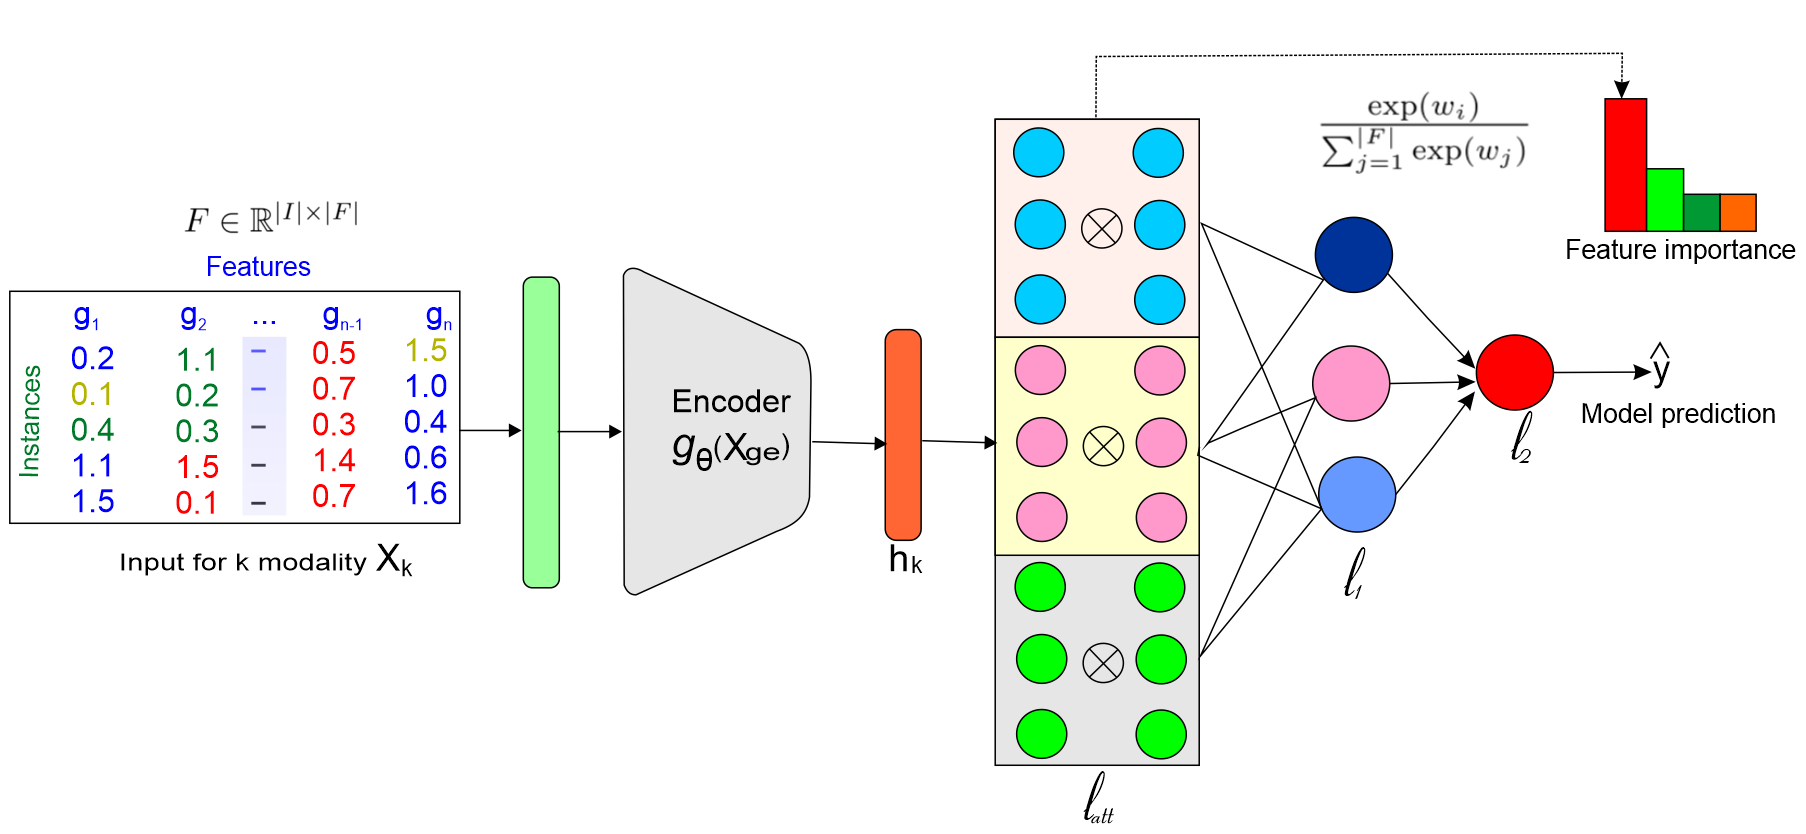
\includegraphics[scale=0.55]{images/k_attention.png}
	\caption{Modality specific attention mechanism on encoder's bottleneck layer for modality `k'}	
	\label{fig:k_attention}
\end{figure*}

\hspace*{3.5mm} The concept of the global attention layer SAN can be used to compute  global feature importance only. %, similar to \cref{eq:gal_k}.
However, it cannot be used to compute modality-specific feature importance. Therefore, the attention mechanism is applied to each modality specific encoder's bottleneck layer, which forms an attention layer, as shown in \cref{fig:k_attention}. The output of the attention layer is an attention weight vector, which is decomposed to compute modality specific feature attributions.
%n contrast, no aggregation is used in global attention layer-based feature importance computation. 
Modality specific latent feature space $h_k$ is used as the input to the attention layer. Let's $g_l$ represents the attention neural network layer, which maintains the connection between the latent features $F_l$ as follows: 

\begin{equation}
    g_l(h)=\frac{1}{k} \bigoplus_{k}\left[h \otimes \operatorname{softmax}\left(W_{l_{\mathrm{att}}}^{k} h+\boldsymbol{b}_{l_{\mathrm{att}}}^{k}\right)\right],
\end{equation}

\hspace*{3.5mm} where $h$ is used as input to a softmax-activated layer by setting the number of neurons equal to the number of features $|F_l|= p \times q $~(i.e., dimension of latent input), $k$ is the number of attention heads, $\otimes$ is the Hadamard\footnote{The Hadamard product is a binary operation, which takes two matrices of the same dimensions and produces another matrix of the same dimension.} product~\cite{horn1990hadamard}, $\oplus$ is the Hadamard summation across individual heads, and $\sigma$ is the ELU activation function. The softmax function applied to $j_{i}$-th element of a weight vector $v_l$ is defined as~\cite{vskrlj2020feature}:

\begin{equation}
    \operatorname{softmax}\left(\boldsymbol{v_l}_{j_{i}}\right)=\frac{\exp \left(\boldsymbol{v_l}_{j_{i}}\right)}{\sum_{j=1}^{|F_l|} \exp \left(\boldsymbol{v_l}_{j}\right),}
\end{equation}

\hspace*{3.5mm} where $v_l \in \mathbb{R}^{|F_l|}$. As $\sigma$ maintains a bijection between $F_l$ and weights in individual heads $W_{latt}^{k}$, weights in the $|F-l| \times|F_l|$ weight matrix represent the relations between features. Then element-wise product with the input space is computed in the forward pass towards predicting the label $\hat{y}$ of individual samples against true label ${y}$. Then similar to SAN, a fully connected softmax layer is used for the classification. Then, similar to SAN, attention vectors from $l_{\text {att}}$ is then used to compute feature importance estimates using a global attention layer, where the weights are activated using softmax activation. 

\begin{sidewaysfigure*}
	\centering
	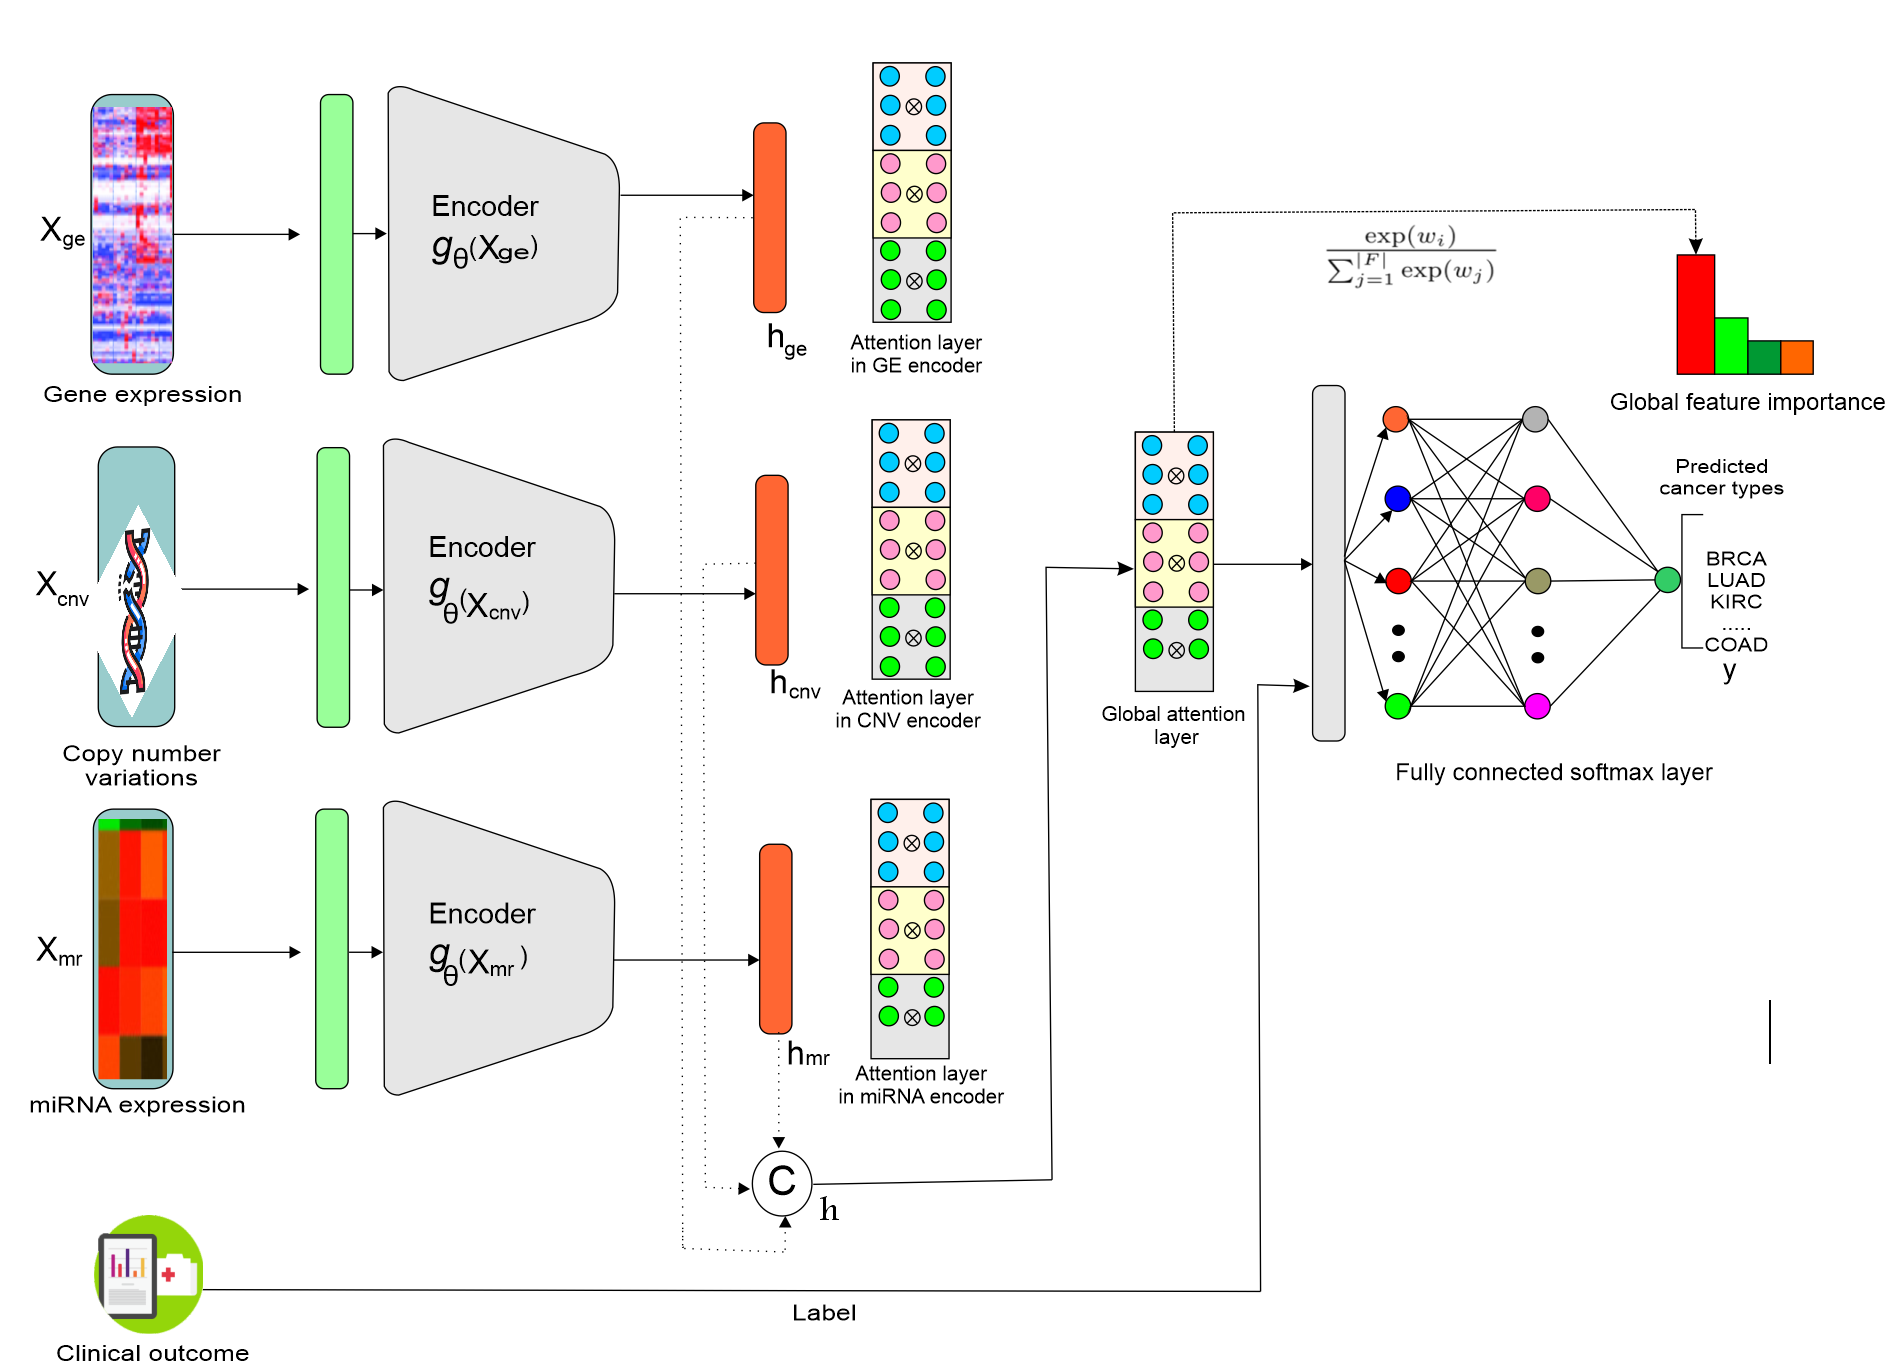
\includegraphics[scale=0.8]{images/full_attention.png}
	\caption[The schematic representation of the overall approach]{The schematic representation of the overall approach, showing global attention mechanism on multimodal input}
	\label{fig:all_attention}
\end{sidewaysfigure*}

\hspace*{3.5mm} On the other hand, similar to SAN's global attention mechanism, another attention layer is applied on top of the final concatenated latent space. This way, the attention layer will then act as a global attention layer, which takes the concatenated~(either based on LRC or SLR) to compute overall feature attributions, as shown in \cref{fig:all_attention}. In both modality specific and final concatenated latent space, feature importance is then computed from the weight vector, similar to SAN as follows~\cite{vaswani2017attention}:

\begin{equation}
    R_{l}=\frac{1}{k} \bigoplus_{k}\left[\operatorname{softmax}\left(\operatorname{diag}\left(W_{l_{\mathrm{att}}}^{k}\right)\right)\right] ; W_{l_{\mathrm{att}}}^{k} \in \mathbb{R}^{|F_l| \times|F_l|},
    %\label{eq:gal_k}
\end{equation}

\hspace*{3.5mm} where the softmax is applied for each feature w.r.t. the remainder of the features. The feature importance is extracted as the main diagonal of the weight matrix, $\operatorname{diag}$. 

%after the last convolutional layer of each CAE encoder for individual modalities. 
%such that the attention vector~(that represents individual feature weights) for each input modality contribute to the latent space $Z_k$.  

\section{Measuring Explainability}
Comprehensiveness, sufficiency, and SCS are computed to measure the quality of the explanation. First, to measure comprehensiveness, a contrast example $\tilde{x}_{i}$ is created, for each sample $x_{i}$, where $\tilde{x}_{i}$ is calculated by removing the predicted rationales $r_{i}$ from $x_{i}$. Let $f\left(x_{i}\right)_{c}$ be the original prediction probability provided by a model $f$~(i.e., $MCAE_{lrc}$ or $MCAE_{slr}$) for the predicted class $c$. If a model $f$ is defined as $f\left(x_{i} \backslash r_{i}\right)_{c}$ as the predicted probability of $\tilde{x}_{i}\left(=x_{i} \backslash r_{i}\right)$, it is expected that the model prediction to be lower on removing the rationales~\cite{deyoung2019eraser}. Then the comprehensiveness $e$ is calculated as~\cite{deyoung2019eraser}: 

\begin{align}
    e  = f\left(x_{i}\right)_{c}-f\left(x_{i} \backslash r_{i}\right)_{c}.
\end{align}

\hspace*{3.5mm} Zaidan E. et al.~\cite{zaidan2007using} introduced the concept of rationales in NLP in which human annotators would highlight a part of text that could support their labeling decision. For example, to justify why a review about a movie is positive, an annotator can highlight the most important words and phrases that would tell someone why to see the movie. While to justify why a review is negative, the annotator can highlight words and phrases that would recommend someone why not to see the movie. It is found to be useful in different NLP tasks~\cite{deyoung2019eraser} like sentiment analysis, hate speech detection, and text classification~\cite{herrewijnenmachine}. 

\hspace*{3.5mm} For the cancer diagnosis, the same idea is conceptualized based on the leave-one-feature-out analysis in which the rationale is computed based on the number of extracted features divided by the number of features in a test sample. A prediction is considered a match if the overlap with any of the ground truth rationales $r_i \geq 0.25$. A high value of comprehensiveness implies that the rationales were influential w.r.t prediction. The sufficiency $s$ measuring the degree to which extracted rationales are adequate for the model $f$ to make a prediction is defined  as follows~\cite{deyoung2019eraser}: 

\begin{align}
    s  =  f\left(x_{i}\right)_{c} f\left(r_{i}\right)_{c}.
\end{align}

\hspace*{3.5mm} SCS is computed w.r.t usability perspective, i.e., based on the response from the usability questionnaires:  

\begin{enumerate}[noitemsep]
    \item \textbf{Factors in data} - I found that data included all relevant known causal factors with sufficient precision and granularity.
    \item \textbf{Understood} - I understood the explanations within the context of my work.
    \item \textbf{Change detail level} - I could change the level of detail on demand.
    \item \textbf{Need teacher/support} - I did not need support to understand the explanations.
    \item \textbf{Understanding causality} - I found the explanations helped me to understand causality.
    \item \textbf{Use with knowledge} - I was able to use the explanations with my knowledge base.
    \item \textbf{No inconsistencies} - I did not find inconsistencies between explanations.
    \item \textbf{Learn to understand} - I think that most people would understand the explanations quickly.
    \item \textbf{Needs references} - I did not need more references in the explanations: e.g., medical guidelines.
    \item \textbf{Efficient} - I received the explanations in a timely and efficient manner.
\end{enumerate}

\hspace*{3.5mm} The SCS recommended a 5 point scale, where rating 1 = strongly disagree, 2 = disagree, 3 = neutral, 4 = agree, 5 = strongly agree. Upon received the feedback on these aspects, SCS is measured by dividing ratings with the total ratings, i.e., $SCS  = \sum_{i=1}^{10} \text {Rating}_{i} / 50$. 

\section{Experiments}\label{chapter_5:results} 
In this section, evaluation results of several experiments are discussed both quantitatively and qualitatively. A comparative analysis with state-of-the-art approaches is provided. To improve the interpretability of the models, experiments are carried out with the following objectives:

\begin{enumerate}[noitemsep]
    %\item What types of neural network architectures are for more for handing multimodal inputs. 
    \item What individual genomic modalities are more suitable for global and individual diagnosis? 
    \item What multimodal input combinations are more suitable for global and individual diagnosis?
    \item Which interpretability technique is more helpful for explaining global and individual diagnosis?
    \item How faithful are the explanations? 
    \item What is more important: accuracy, explainability, or faithfulness?
\end{enumerate}

\hspace*{3.5mm} Results of each observation is analysed, both quantitative and qualitatively. 

\subsection{Experiment setup}
Each network is trained for 500 epochs, in a similar setting of cosine annealing cycling, by setting the batch size to $128$. The activity regularization term $\lambda$ is set between $[0.001, 0.005]$, while the regularization weights of the loss functions in \cref{eq:sum} are set as  $\alpha_{r}$=0.1, and $\alpha_{c}$=0.25. Further, the effect of minor noise~(by leveraging a Gaussian noise layer) and dropout regularization are observed. Gaussian noise parameters are empirically set to a standard deviation of 0.1 and a mean of 0.

\hspace*{3.5mm} Results based on random hyperparameters search and 5-fold cross-validation are reported with macro-averaged precision and recall. Since the dataset is moderately imbalanced, Matthias correlation coefficient~(MCC) scores are reported. We did not report F1-scores since they are significant only when precision and recall are very different. Thus, it is important for cancer diagnosis to have both high precision and high recall~\cite{naulaerts2017precision}, results with very different precision and recall are not useful in cancer diagnosing and tumor type identification. Besides, we report the comprehensiveness and sufficiency to measure the faithfulness of the explanations and the predictions. 

%Hence, we did not report F1-scores. 
\hspace*{3.5mm} When we create snapshots, we set the number of epochs to 200, maximum LR to 1.0, and the number of cycles to 20, giving 20 snapshots for each model. For 4 different architectures~(vanilla CNN, VGG16, $MCAE_{lrc}$, and $MCAE_{slr}$), we get 80 snapshot models in total, on which we construct the ensemble prediction on. Two best snapshot models are then used for the decision visualization and evaluations. Besides, a web application is developed, based on $MCAE_{lrc}$ classifier. The idea is to explain the diagnosis, via 6 different areas, namely: i) Global explanations, ii) Local explanations, iii), Feature interactions, iv) Data distributions, v) Model performance, and vi) Measure of explainability. %, as shown in \cref{fig:ui_explain}. 

\iffalse
\begin{sidewaysfigure*}
\centering
	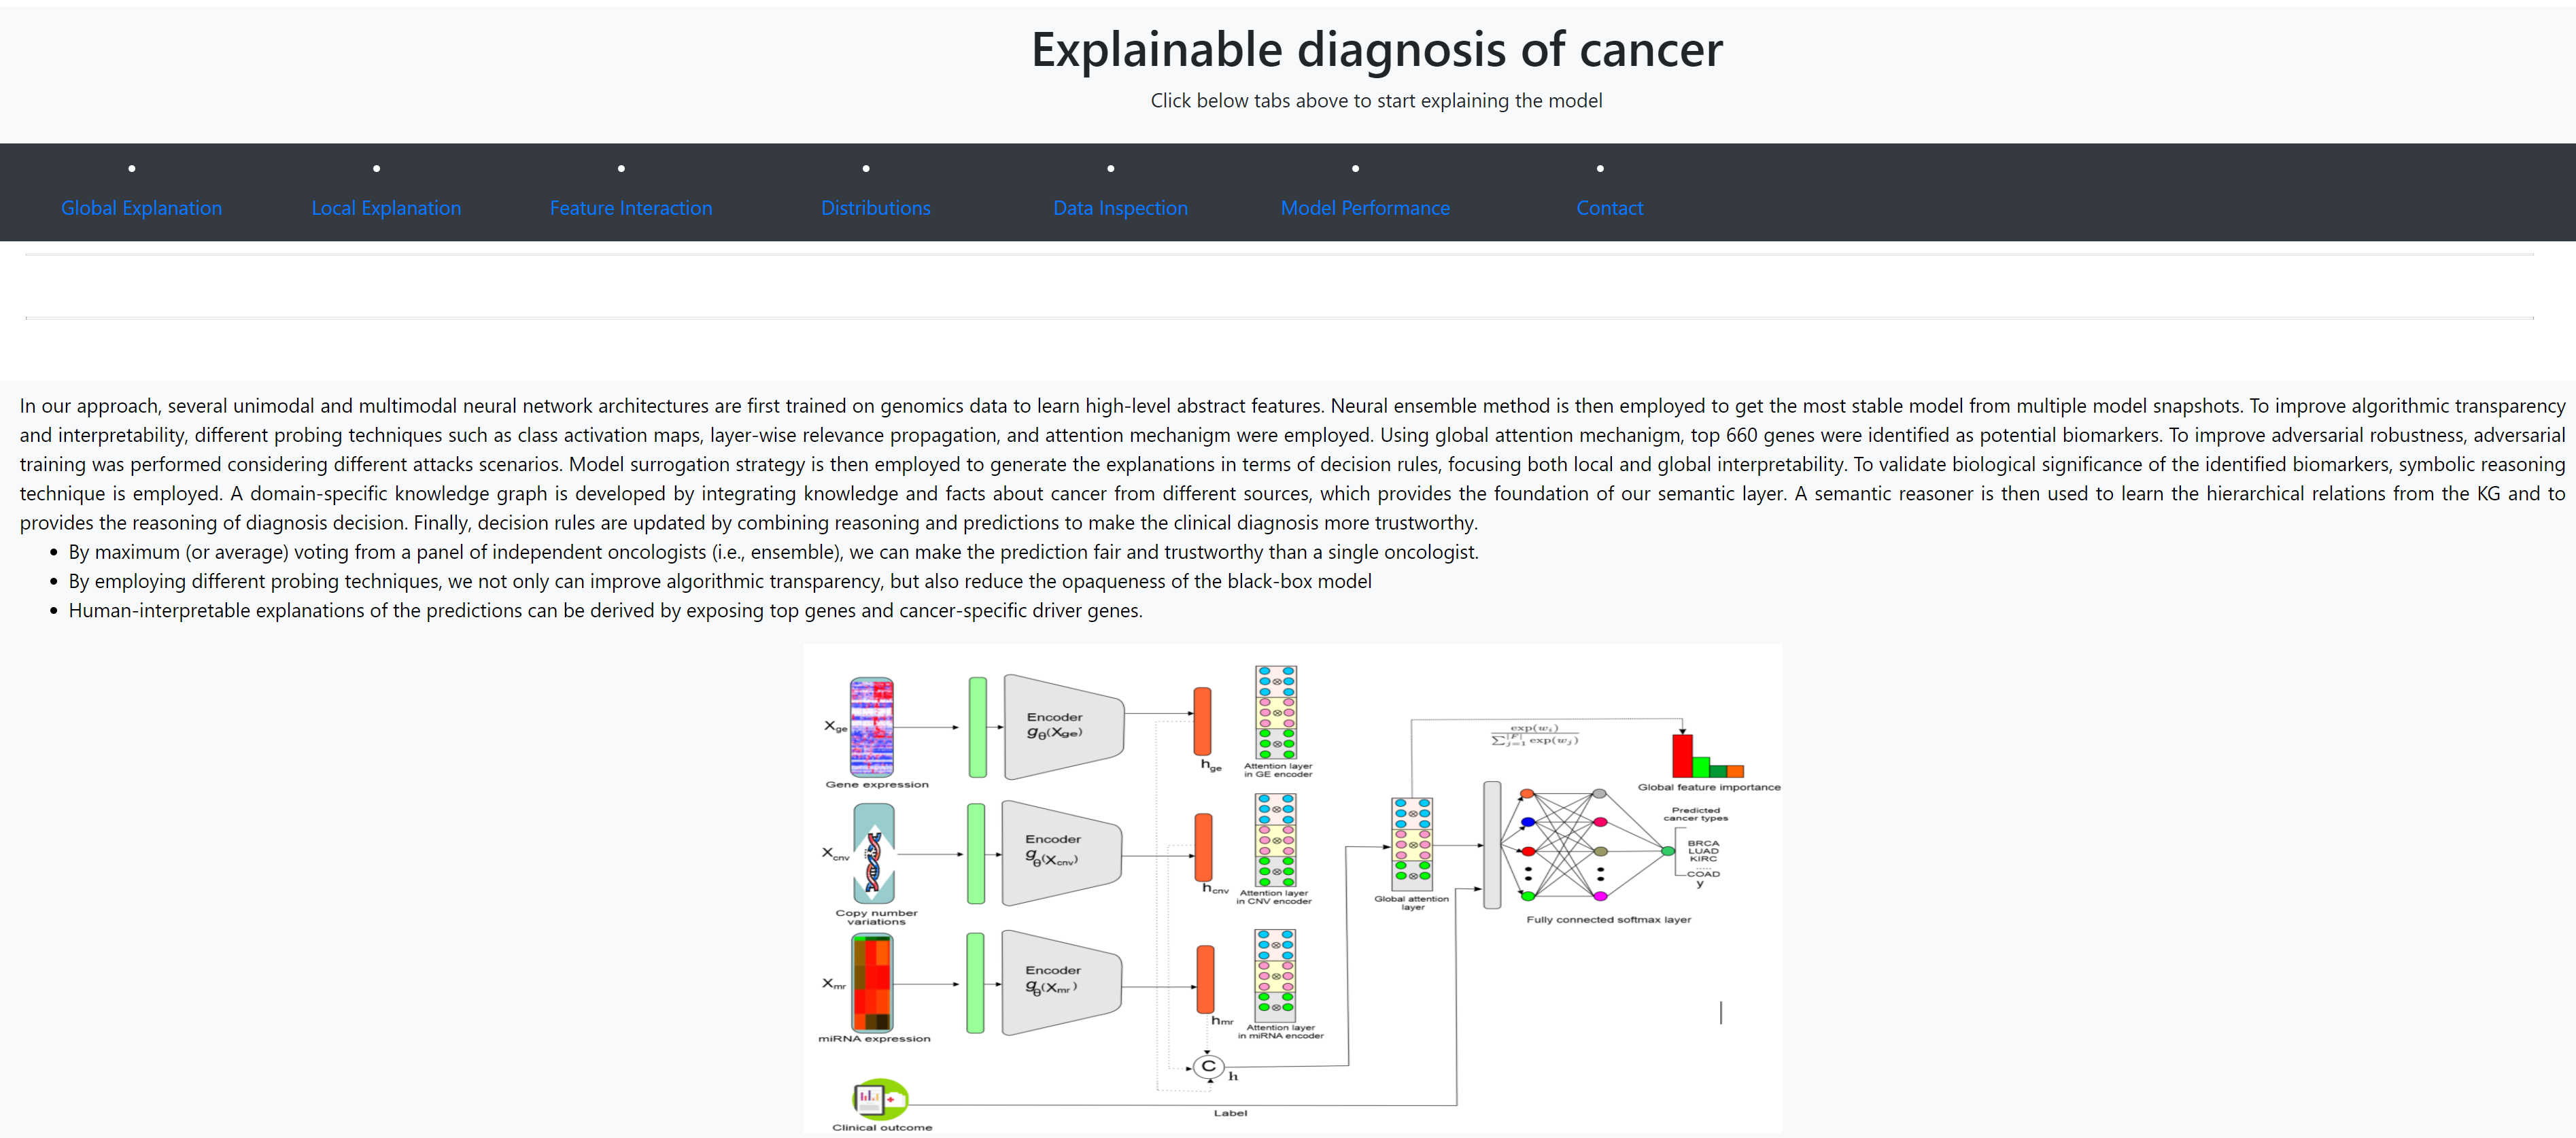
\includegraphics[scale=0.8]{images/ui.png}
	\caption{High-level user interface to explain the predictions}
    \label{fig:ui_explain}
    \vspace{-4mm}
\end{sidewaysfigure*}
\fi 

\subsection{Model performance}
In this sub-section, we analyse performance of each model, considering both single and multimodality. Then, both marker genes and common genes will be selected for the model surrogate strategy in \cref{chapter:xai_rules}.

\subsubsection{Model performance: single modality}
The average accuracy obtained was 89.75\% and 96.25\% using CNN and VGG16 models, respectively. However, since the classes are imbalanced, only the accuracy will give a very distorted estimation of the cancer types. Thus, we report the class-specific classification reports along with the corresponding MCC scores in \cref{table:class_specific}. As can be seen, precision and recall for the majority cancer types were high and for these the VGG16 model performs mostly better. Notably, the VGG16 model classifies BRCA, UCEC, LUAD, HNSC, LUSC, THCA, PRAD, BLCA, STAD, KIRC, LIHC, COAD, CESC, KIRP, SARC, OV, PCPG, TGCT, GBM, READ, LAML, MESO, and DLBC cancer cases more confidently, whereas the CNN model classifies PAAD, CHOL, and UCS cancer cases more accurately. 

\begin{table*}[h]
    \caption{Class-specific performance between CNN vs. VGG16 for cancer type prediction}
      \label{table:class_specific} %RF Confusion Matrix Oncogene Subtype
        \begin{center}
        \vspace{-6mm}
        \scriptsize{
        \begin{tabular}{l|lll|lll}
        \toprule
        %\rowcolor{Gray}
        {} & \multicolumn{2}{c}{\textbf{\hspace{0.7cm} CNN~(89.75\%)}} & \multicolumn{3}{c}{ \textbf{\hspace{1.5cm} VGG16~(96.25\%)}} &  {} \\
        \textbf{Type } & \textbf{Precision} &  \textbf{Recall}  & \textbf{MCC} & \textbf{Precision} &  \textbf{Recall} & \textbf{MCC} \\\midrule%\hline
        BRCA   & {\color{red}\textbf{0.8785}} & 0.8612 & 0.7564 & {\color{red}\textbf{0.9437}} & 0.9511 & 0.8465  \\%\hline
        LGG    & 0.9254 & 0.8926 & 0.8330 & 0.9311 & 0.9402 & 0.8421  \\%\hline
        UCEC   & 0.8753 & 0.8819 & 0.7835 & 0.9562 & 0.9429 & 0.8445  \\%\hline
        LUAD   & 0.8235 & 0.8354 & 0.7136 & 0.9865 & 0.9823 & 0.8624  \\%\hline
        HNSC   & 0.8520 & 0.8743 & 0.7851 & 0.9730 & 0.9822 & 0.8765  \\%\hline
        THCA   & {\color{red}\textbf{0.8528}} & 0.8323 & 0.7275 & {\color{red}\textbf{0.9138}} & 0.9154 & 0.8125  \\%\hline
        PRAD   & {\color{red}\textbf{0.8827}} & 0.8778 & 0.7847 & {\color{red}\textbf{0.9233}} & 0.9347 & 0.8207  \\%\hline
        LUSC   & 0.8726 & 0.8634 & 0.7625 & 0.9434 & 0.9472 & 0.8524  \\%\hline
        BLCA   & 0.8956 & 0.9037 & 0.8075 & 0.9656 & 0.9537 & 0.8475  \\%\hline
        STAD   & 0.8253 & 0.8156 & 0.6932 & 0.9653 & 0.9556 & 0.8532  \\%\hline
        SKCM   & 0.8853 & 0.8711 & 0.8025 & 0.9046 & 0.9136 & 0.8168  \\%\hline
        KIRC   & 0.8967 & 0.9123 & 0.8237 & 0.9578 & 0.9689 & 0.8531  \\%\hline
        LIHC   & 0.8194 & 0.8085 & 0.6945 & 0.9572 & 0.9664 & 0.8537  \\%\hline
        COAD   & 0.8368 & 0.8245 & 0.7679 & 0.9776 & 0.9690 & 0.8514  \\%\hline
        CESC   & 0.8785 & 0.8743 & 0.7964 & 0.9873 & 0.9885 & 0.8664  \\%\hline
        KIRP   & 0.8254 & 0.8032 & 0.7043 & 0.9681 & 0.9782 & 0.8430  \\%\hline
        SARC   & 0.8753 & 0.8671 & 0.7835 & 0.9365 & 0.9435 & 0.8421 \\%\hline
        OV     & 0.8825 & 0.8733 & 0.7936 & 0.9725 & 0.9773 & 0.8262  \\%\hline
        ESCA   & {\color{cyan}\textbf{0.8913}} & 0.8719 & 0.7951 &  {\color{cyan}\textbf{0.8956}} & 0.8834 & 0.8076  \\%\hline
        PCPG   & 0.8537 & 0.8611 & 0.7875 & 0.9875 & 0.9987 & 0.8735  \\%\hline
        PAAD   & 0.9629 & 0.9567 & 0.8407 & 0.9452 & 0.9500 & 0.8325  \\%\hline
        TGCT   & 0.8736 & 0.8722 & 0.7825 & 0.9890 & 0.9724 & 0.8434  \\%\hline
        GBM    & 0.8952 & 0.8845 & 0.8075 & 0.9362 & 0.9453 & 0.8436  \\%\hline
        THYM   & 0.9255 & 0.9123 & 0.8232 & 0.9775 & 0.9678 & 0.8622  \\%\hline
        READ   & {\color{cyan}\textbf{0.6795}} & 0.6857 & 0.6225 & {\color{cyan}\textbf{0.8874}} & 0.8733 & 0.7525  \\%\hline
        LAML   & 0.8697 & 0.8567 & 0.8237 & 0.9576 & 0.9632 & 0.8513  \\%\hline
        MESO   & 0.8991 & 0.9028 & 0.8076 & 0.9534 & 0.9456 & 0.8457  \\%\hline
        UVM    & 0.8765 & 0.8623 & 0.7979 & 0.9136 & 0.9089 & 0.8184  \\%\hline
        ACC    & 0.9217 & 0.9345 & 0.8225 & 0.9623 & 0.9731 & 0.8611  \\%\hline
        KICH   & 0.9335 & 0.9475 & 0.8425 & 0.9690 & 0.9625 & 0.8439  \\%\hline
        UCS    & {\color{cyan}\textbf{0.9157}} & 0.9064 & 0.8125 & {\color{cyan}\textbf{0.8726}} & 0.8675 & 0.7869  \\%\hline
        DLBC   & 0.8678 & 0.8729 & 0.7005 & 0.9347 & 0.9421 & 0.8389  \\%\hline
        CHOL   & {\color{cyan}\textbf{0.8838}} & 0.8975 & 0.7979 & {\color{cyan}\textbf{0.8455}} & 0.8342 & 0.6821  \\%\hline
        \midrule
        %\rowcolor{LightCyan}
        \textbf{Average} &   \textbf{0.8975}    &  \textbf{0.9065} &    \textbf{0.8052}   &  \textbf{0.9625} & \textbf{0.9542} & \textbf{0.8453}\\
        \bottomrule
        \end{tabular}}
        \vspace{-4mm}
    \end{center}
\end{table*}

\begin{sidewaysfigure*}
	\centering
	\begin{subfigure}{.48\linewidth}
		\centering
		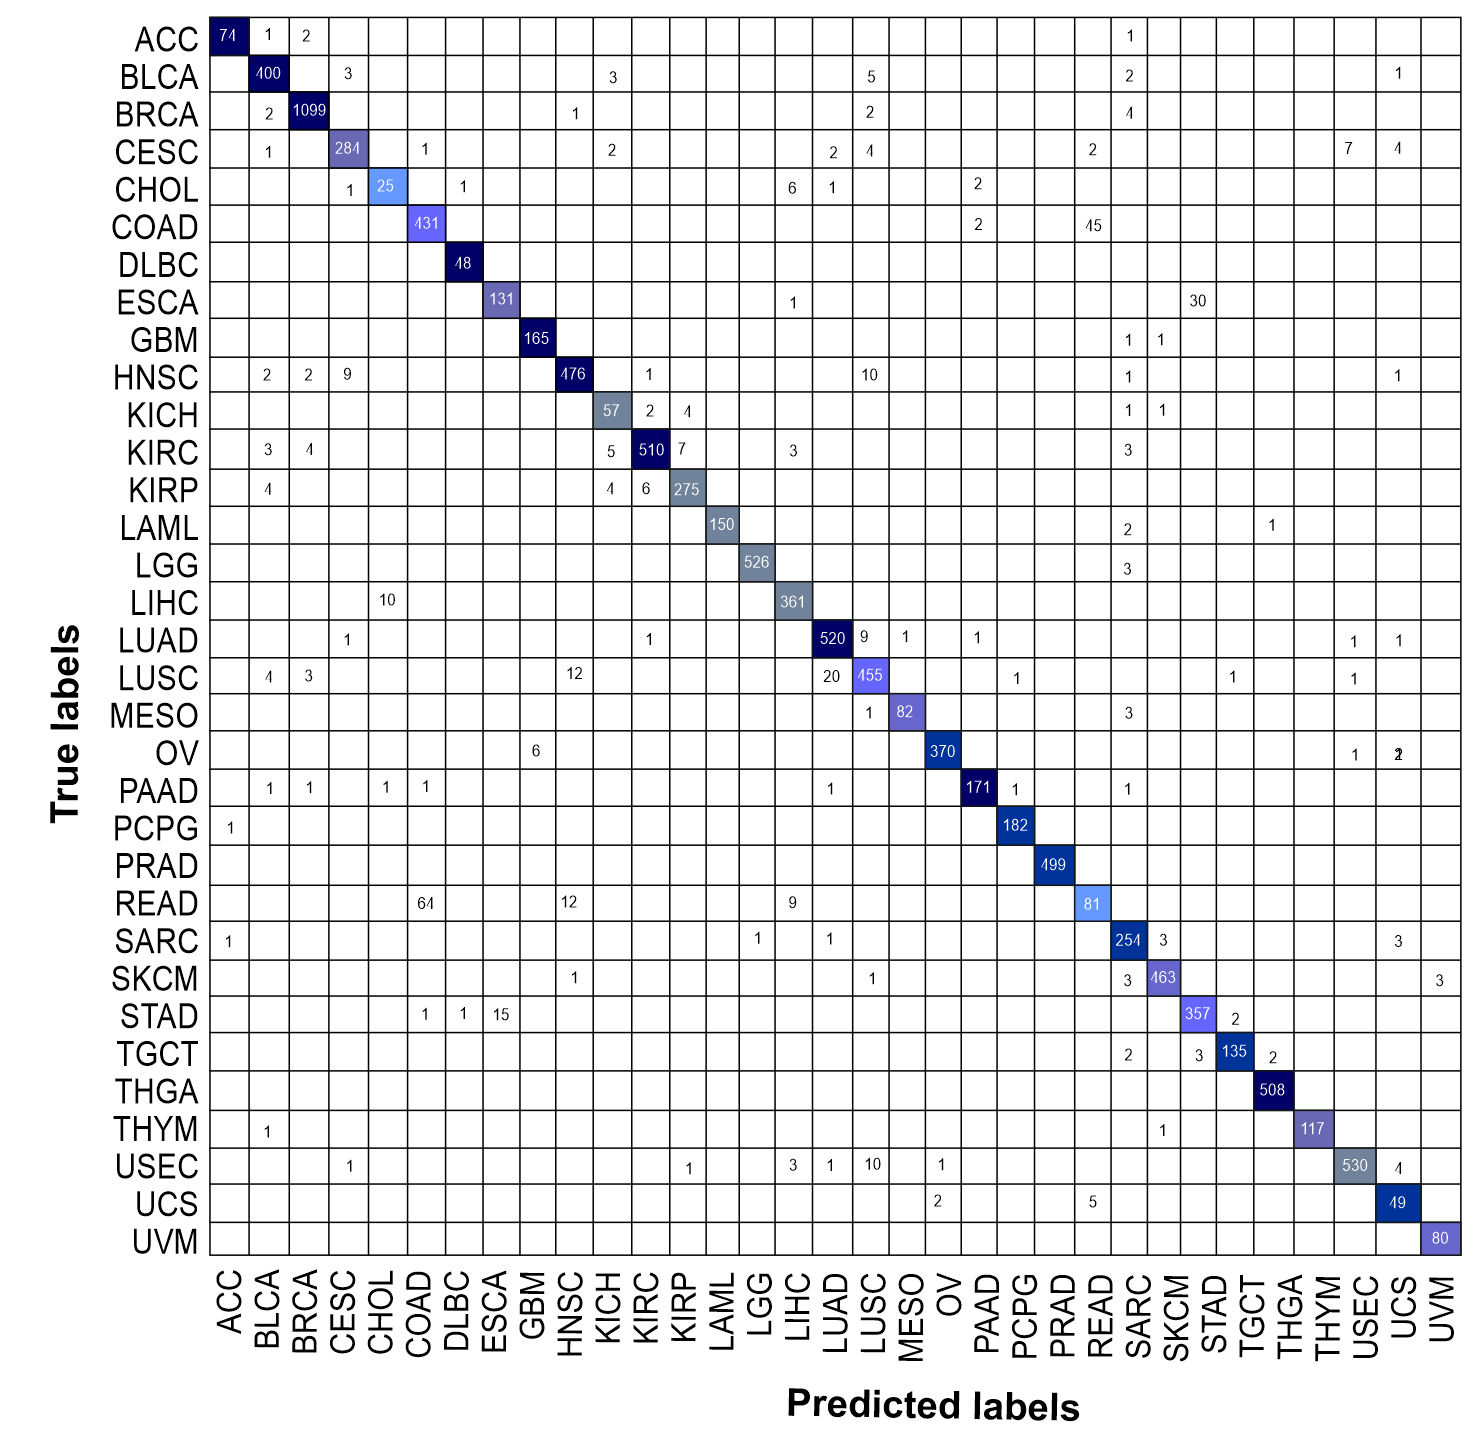
\includegraphics[width=0.8\textwidth,height=100mm]{images/conf_uni_modal.png}
		\caption{Confusion matrix}
        \label{fig:conf_cnn}
	\end{subfigure}
	\hspace{-4mm}
	\begin{subfigure}{0.48\linewidth}
		\centering
		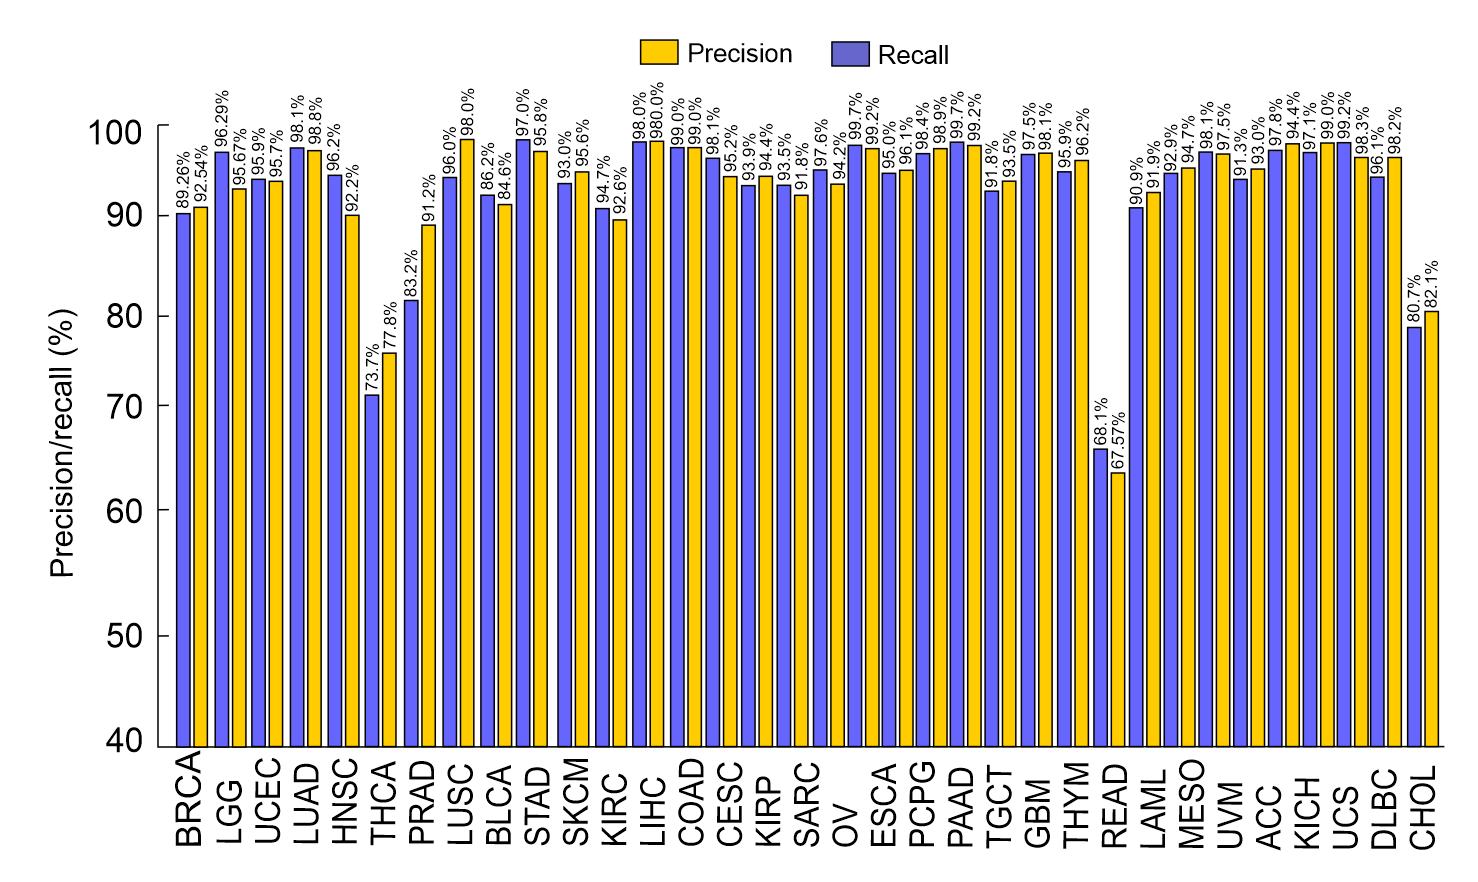
\includegraphics[width=0.9\textwidth,height=100mm]{images/pvr_value.png}
		\caption{Precision and recall}
        \label{fig:pr_vgg16}
	\end{subfigure}
	\caption{Confusion matrix, precision, and recall for VGG16 model.} 
	\label{fig:conf_precision_recall_vgg16}
	\vspace{-4mm}
\end{sidewaysfigure*}

\iffalse
\begin{figure*}[h]
\centering
	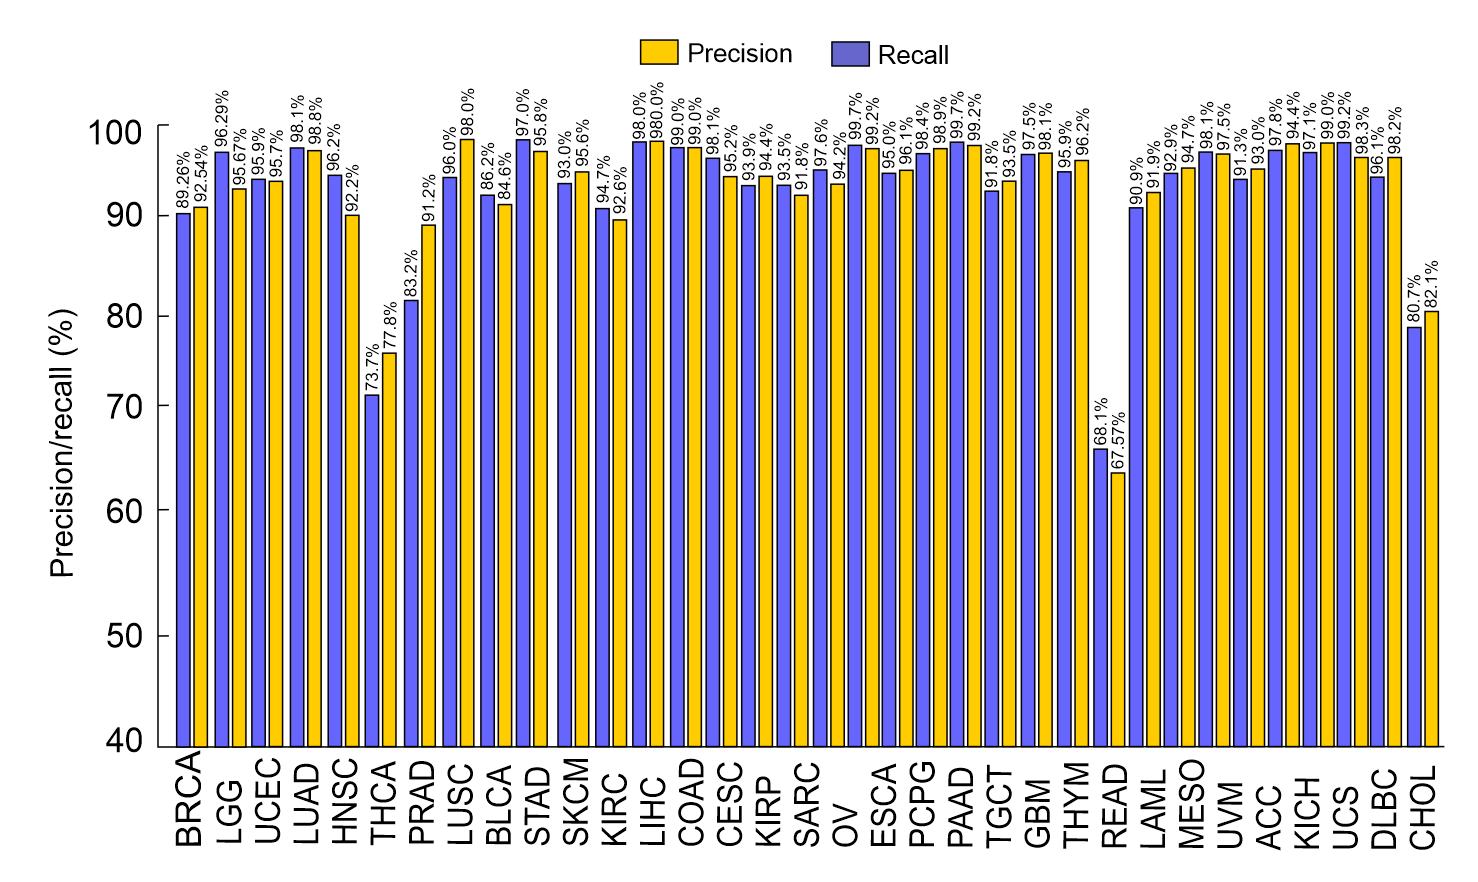
\includegraphics[scale=0.6]{images/pvr_value.png}
	\caption{Precision and recall of VGG16 model}
    \label{fig:pr_vgg16}
    \vspace{-4mm}
\end{figure*}
\fi 

\hspace*{3.5mm} The downside is that both classifiers made substantial mistakes, e.g., VGG16 could classify HNSC and LUSC tumor samples accurately in only 79\% and 81\% of the cases. On the other hand, the CNN model made more mistakes particularly on the STAD, HNSC, LUSC, and LGG tumor samples. In summary, both classifiers performed moderately well except for certain types of tumor cases such as STAD, HNSC, BLCA, THCA, UCEC, LUAD, LUSC, and LGG. The ROC curves generated by the VGG16 model 
%in \cref{fig:both_dataset} 
show that the AUC scores are consistent across the folds showing stable predictions, which shows about 5\% boost in AUC scores generated by the VGG16 model. This signifies that the predictions by the VGG16 model are much better than random guessing. 

\iffalse
\begin{figure*}[h]
    \centering
	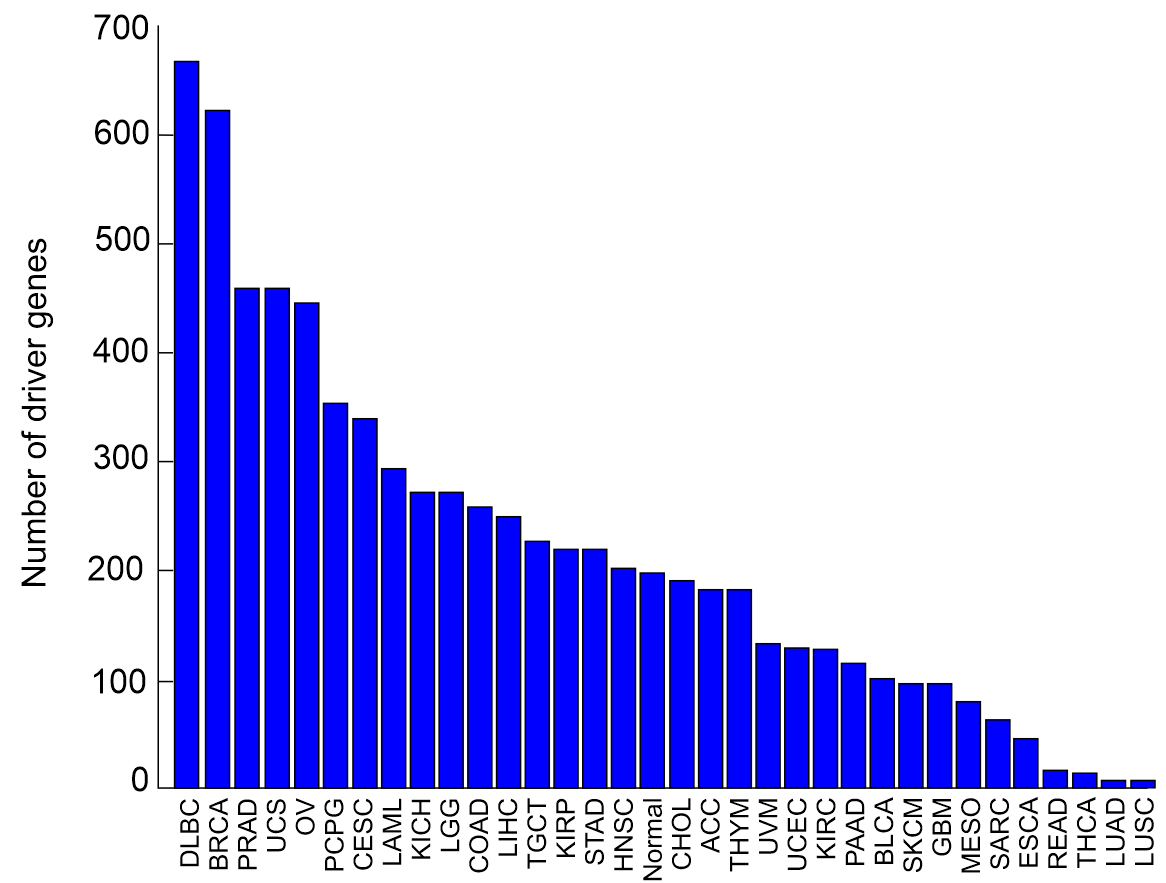
\includegraphics[width=0.8\linewidth,height=70mm]{images/driver_genes.png}
	\caption{Marker genes identified by vanilla CNN per class with a gene effect score of minimum 0.3}
    \label{fig:dg_cnn}
\end{figure*}
\begin{figure*}[h]
\centering
	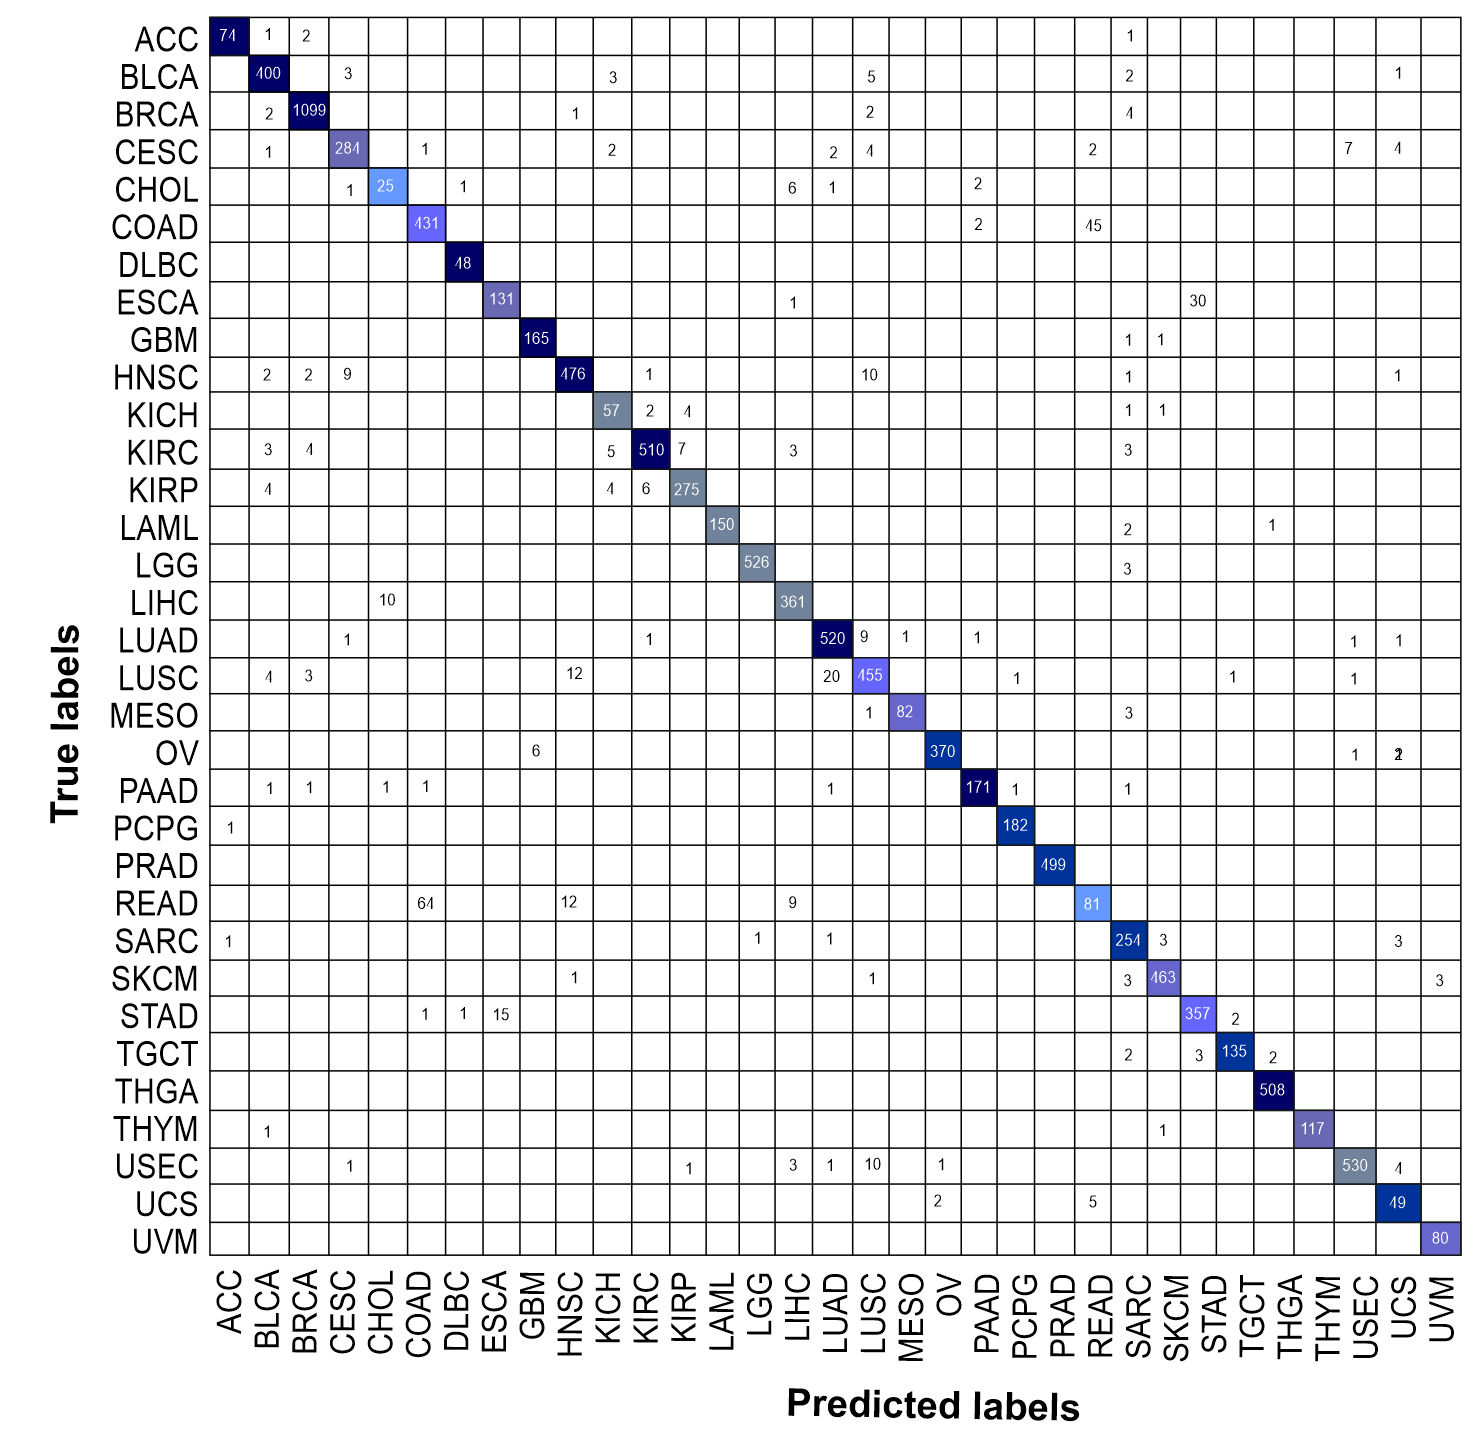
\includegraphics[scale=0.5]{images/conf_uni_modal.png}
	\caption{Confusion matrix of the VGG16 model}
    \label{fig:conf_cnn}
    \vspace{-4mm}
\end{figure*}

\begin{figure*}
	\centering
	\begin{subfigure}{.48\linewidth}
		\centering
		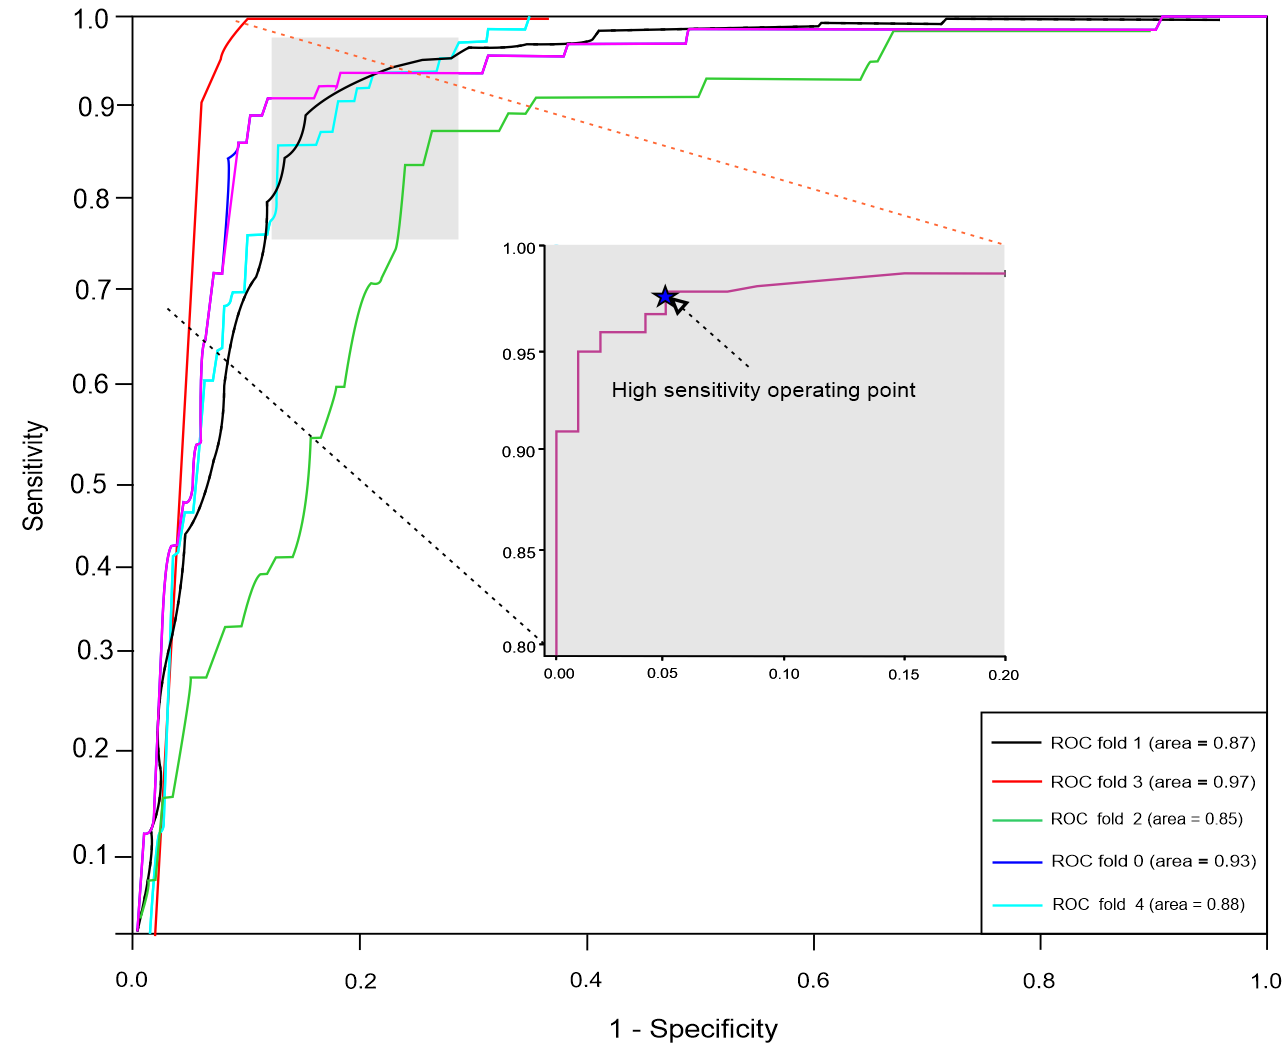
\includegraphics[scale=0.7]{images/roc_1000_genome.PNG}
		\caption{CNN}
        \label{fig:roc_cnn}
	\end{subfigure}
	\hspace{2mm}
	\begin{subfigure}{0.48\linewidth}
		\centering
		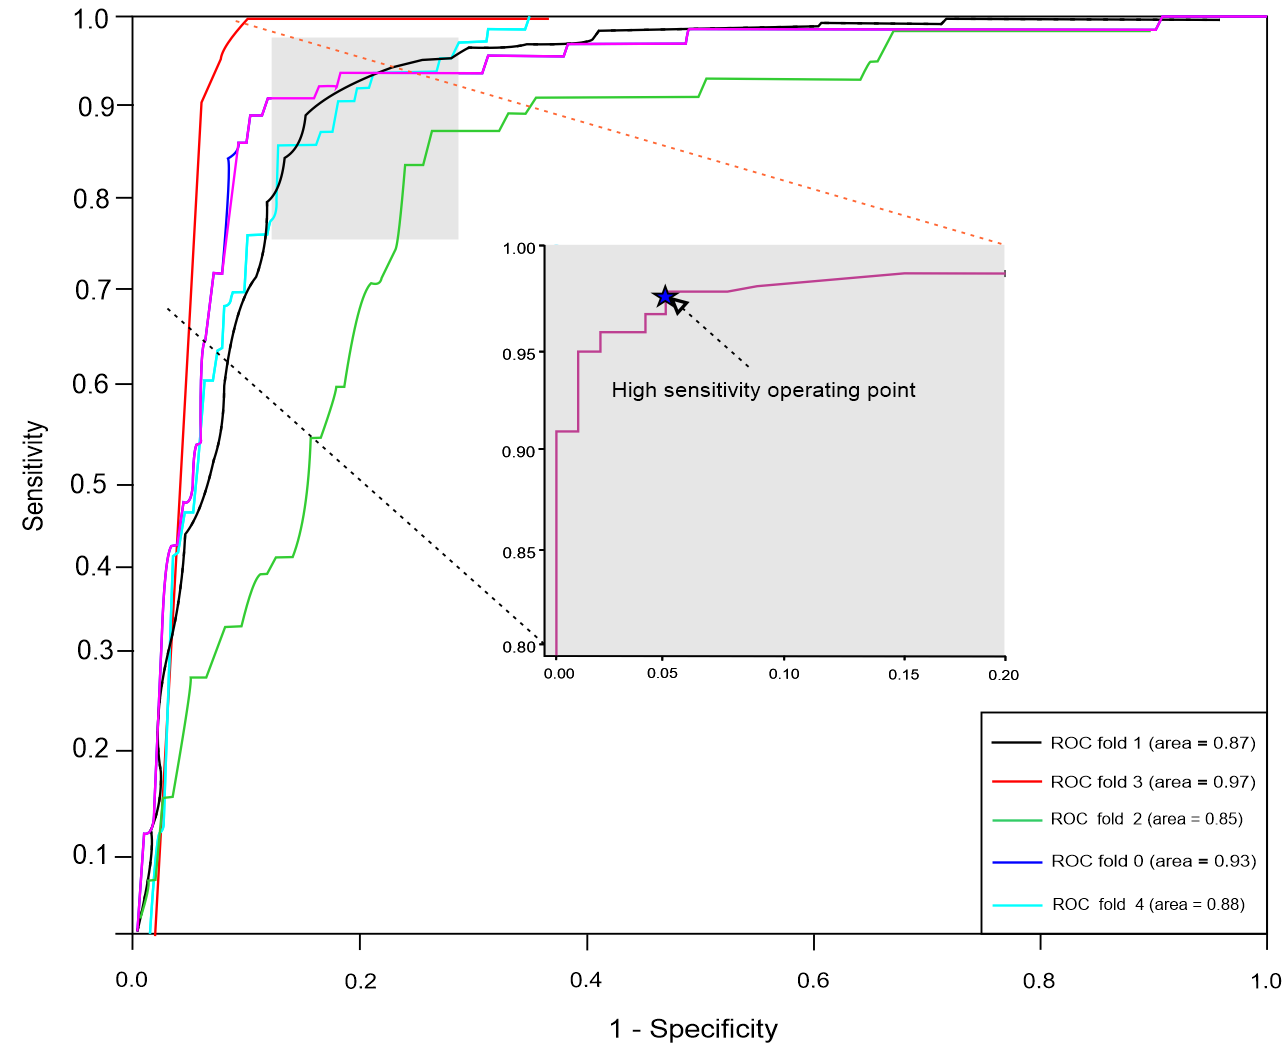
\includegraphics[scale=0.7]{images/roc_1000_genome.PNG}
		\caption{VGG16}
        \label{fig:roc_vgg16}
	\end{subfigure}
	\caption{ROC curves of the vanilla CNN and VGG16 models across folds.} 
	\label{fig:rocs}
	\vspace{-4mm}
\end{figure*}
\fi 

\hspace*{3.5mm} Further, class-specific MCC scores of the VGG16 model are 4\% higher than the CNN model, which suggests that the predictions were strongly correlated with the ground truth, yielding a Pearson product-moment correlation coefficient higher than 0.70 for all the classes except for the CHOL tumor samples. The downside, however, is that both classifiers made a number of mistakes too, e.g., VGG16 can classify ESCA, READ, UCS, and CHOL tumor cases in only 89\% of the cases accurately, while the CNN model made more mistakes particularly for the READ, LUAD, LIHC, KIRP, COAD, and STAD tumor samples. Nevertheless, as is shown 17 of 23 normal classes are classified into their corresponding cancer type, where normal samples from kidney~(KICH, KIRC and KIRP), liver~(CHOL and LIHC), lung~(LUAD and LUSC) or digestive system~(ESCA and STAD) are clearly grouped together. This indicates probably the model learned to recognize tissues of origin. While we analysed the classification results of tumor samples, the major classification errors are also within kidney, lung, colon, and rectum adenocarcinomas.

\begin{sidewaysfigure*}
	\centering
	\begin{subfigure}{.48\linewidth}
		\centering
		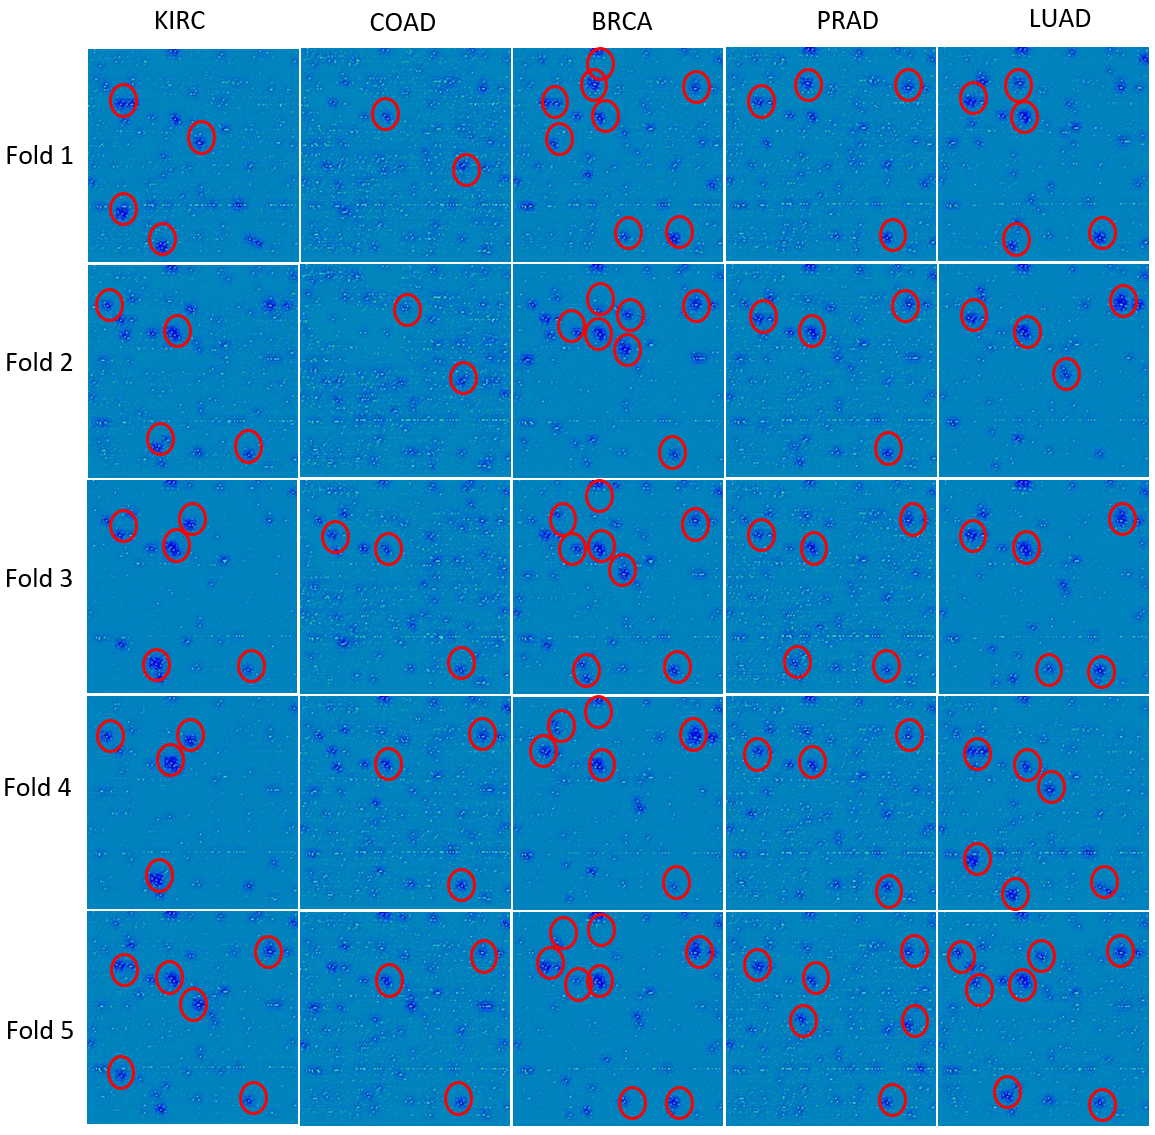
\includegraphics[scale=0.9]{images/gcam+.png}
		\caption{Grad-CAM++}
        \label{fig:hm_gcam++}
	\end{subfigure}
	%\hspace{2mm}
	\begin{subfigure}{0.48\linewidth}
		\centering
		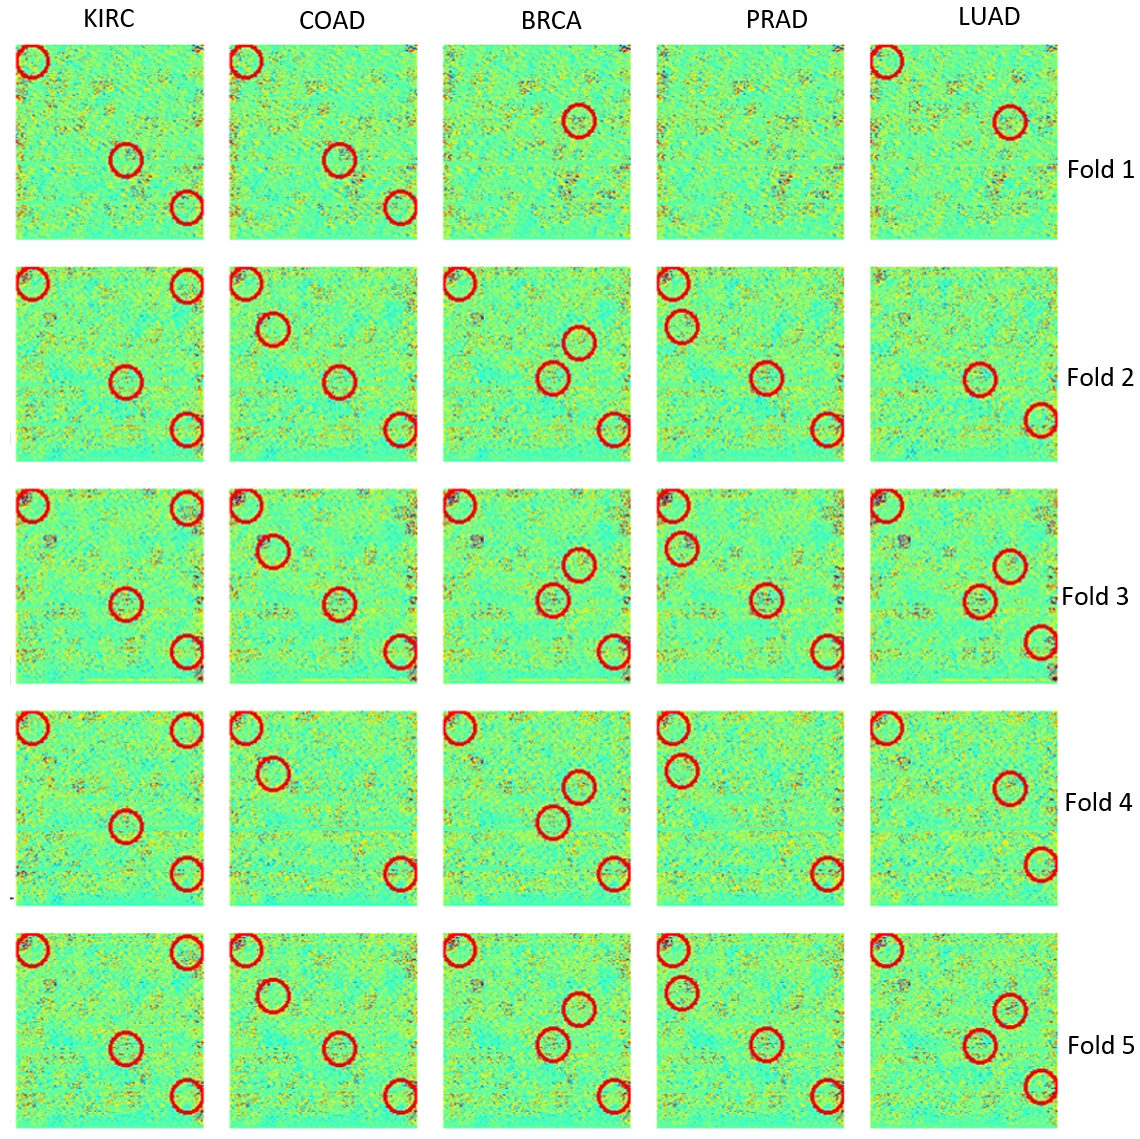
\includegraphics[scale=0.9]{images/lrp_viz.png}
		\caption{LRP}
        \label{fig:lrp}
	\end{subfigure}
	\caption[Heatmap example to mark driver biomarker for different cancer types]{Heat map examples based on Grad-CAM++ and LRP that highlight driver biomarkers for BRCA, KIRC, COAD,\\ LUAD, and PRAD cancer types. Gene positions on 2D pixel space are marked with red circle~(genes may overlap in\\ the marked region). Here, rows represent folds,  columns cancer types.} 
	\label{fig:hm_all}
	\vspace{-2mm}
\end{sidewaysfigure*}

%This part still needs to be calculated and updated 
\subsubsection{Model performance: multimodality}
The average accuracy and F1-scores by the multimodal $MCAE_{lrc}$, and $MCAE_{slr}$ models are slightly lower than the single networks. Still, $MCAE_{lrc}$ gave competitive results compared to vanilla CNN and VGG16 with a single type of input as well as $MCAE_{slr}$ for most of the cancer types. 
%as well as other best ML baselines, e.g., GBT and RF. 
In particular, GE + miRNA expression giving the best results for the classification.
%and decent results for survival rate prediction. 
Overall, both $MCAE_{lrc}$ and $MCAE_{slr}$ models better than that of MAE because of three main reasons: i) number of samples across modalities have been increased 1000 vs 10,000, ii) the reconstruction errors for both multimodal architectures based on CAE have decreased, iii) compared to ML baselines and MAE model, both $MCAE_{lrc}$ and $MCAE_{slr}$ models can learn more complex concepts from the GE + miRNA multimodal features. This results in a lower bias, which can be observed from higher training scores than the validation scores for the maximum number of samples i.e. adding more training samples does increase model generalization. 

\hspace*{3.5mm} Nevertheless, the latter two reasons helped improve the generalization by mitigating both bias and variance errors. However, we closely observed the performance of $MCAE_{lrc}$ and $MCAE_{slr}$ models. We found that $MCAE_{lrc}$ model based on LRC clearly outperforms the $MCAE_{slr}$ model. Further, we perform the Wilcoxon signed rank test with a significance level of 5\%. Then it becomes more evident from the comparison of reconstruction losses and accuracies for $MCAE_{lrc}$ and $MCAE_{slr}$ from \cref{fig:ce_multimodal_models_1} and \cref{fig:ce_multimodal_models_2}. Within each box-plot, mean and median values of the reconstruction losses are depicted with a dot and a horizontal line. As seen in \cref{fig:ce_multimodal_models_1} and \cref{fig:ce_multimodal_models_2}, $MCAE_{slr}$ model based on SLR performs worst in each and every combination of input modalities, irrespective of reconstruction loss and f1-score. 

\begin{figure*}
	\centering
	\begin{subfigure}{.48\linewidth}
		\centering
		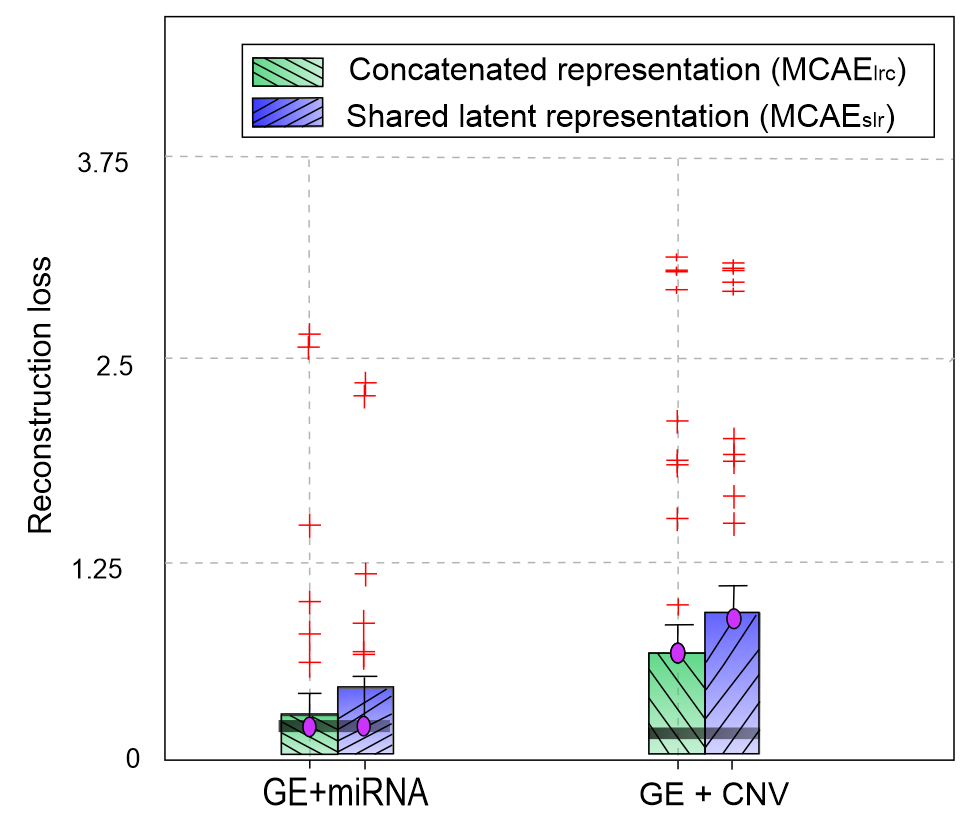
\includegraphics[width=\linewidth,height=60mm]{images/ce_mcae_1.png}
		\caption{GE+miRNA vs. GE+CNV modality}
        \label{fig:ce_ge_mirna}
	\end{subfigure}
	\begin{subfigure}{0.48\linewidth}
		\centering
		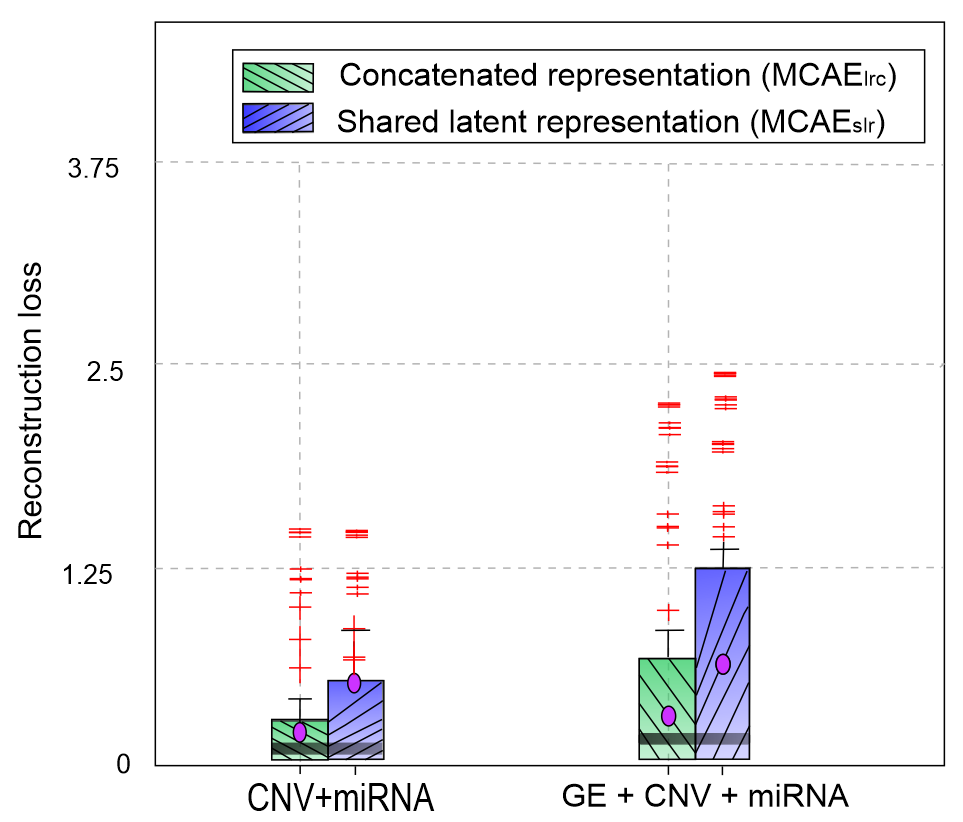
\includegraphics[width=\linewidth,height=60mm]{images/ce_mcae_2.png}
		\caption{CNV+miRNA vs. GE+CNV=miRNA modality}
        \label{fig:ce_ge_cnv}
	\end{subfigure}
	\caption{Comparison of reconstruction losses for $MCAE_{lrc}$ and $MCAE_{slr}$ during pretraining} 
	\label{fig:ce_multimodal_models_1}
\end{figure*}

\begin{figure*}
	\centering
	\begin{subfigure}{.48\linewidth}
		\centering
		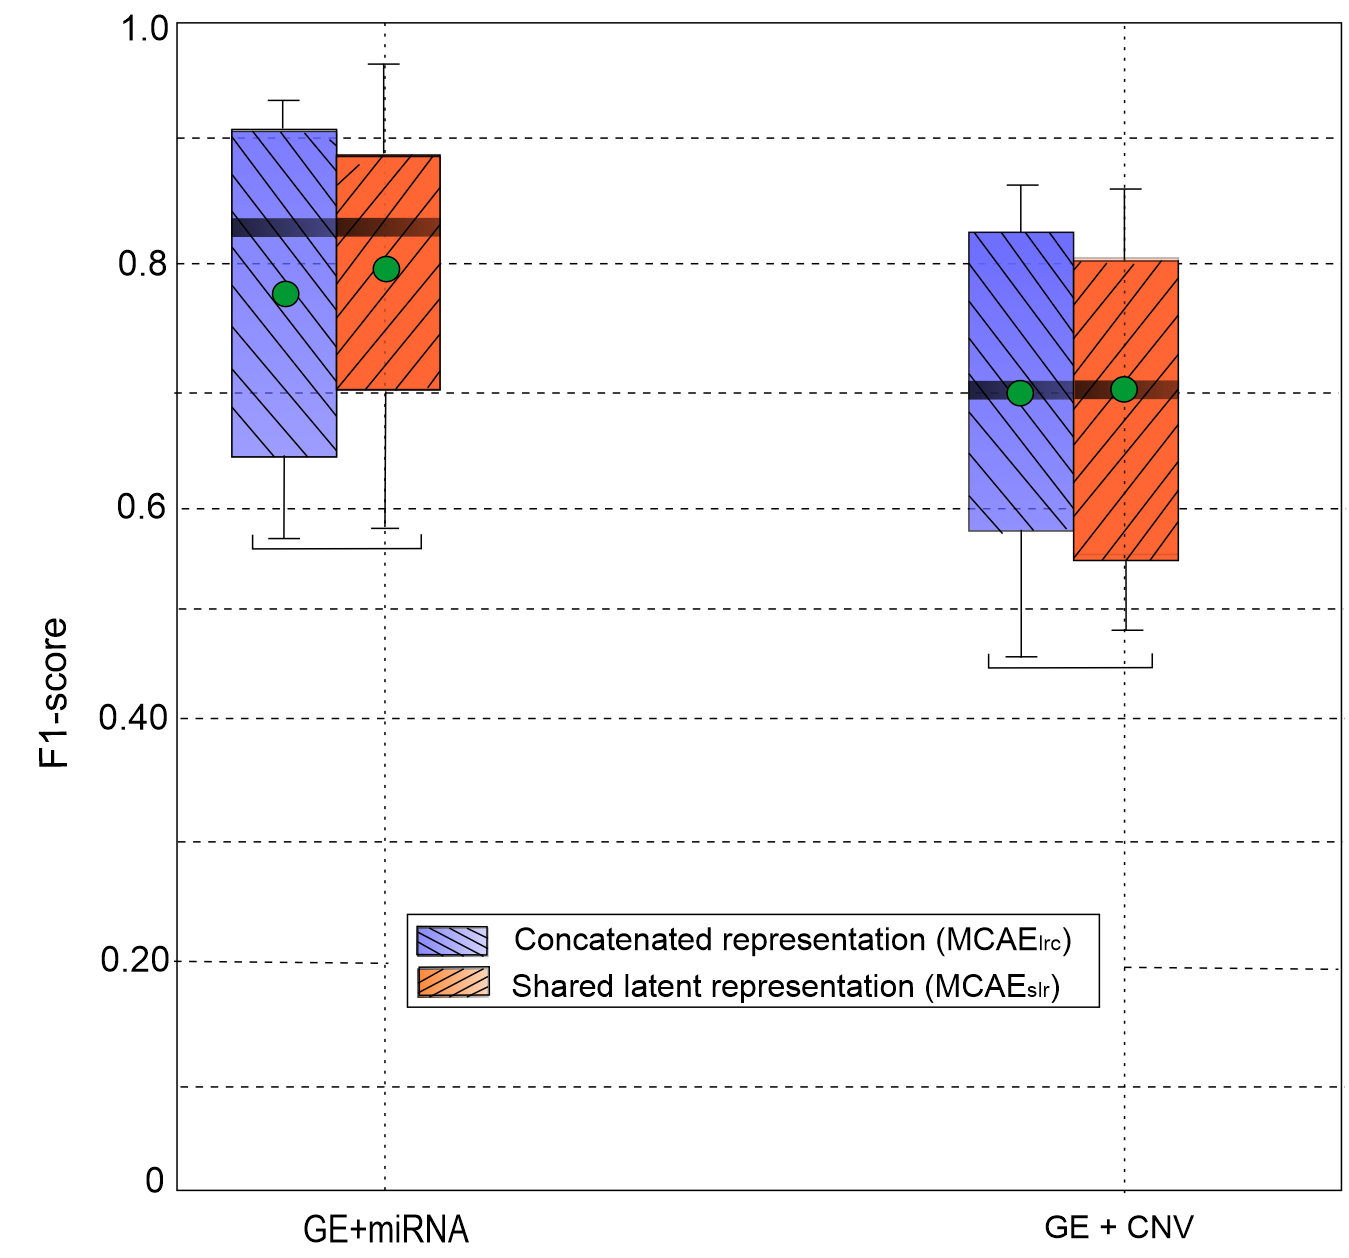
\includegraphics[width=\linewidth,height=55mm]{images/acc_mcae_1.png}
		\caption{GE+miRNA vs. GE+CNV modality}
        \label{fig:ce_ge_mirna_2}
	\end{subfigure}
	\begin{subfigure}{0.48\linewidth}
		\centering
		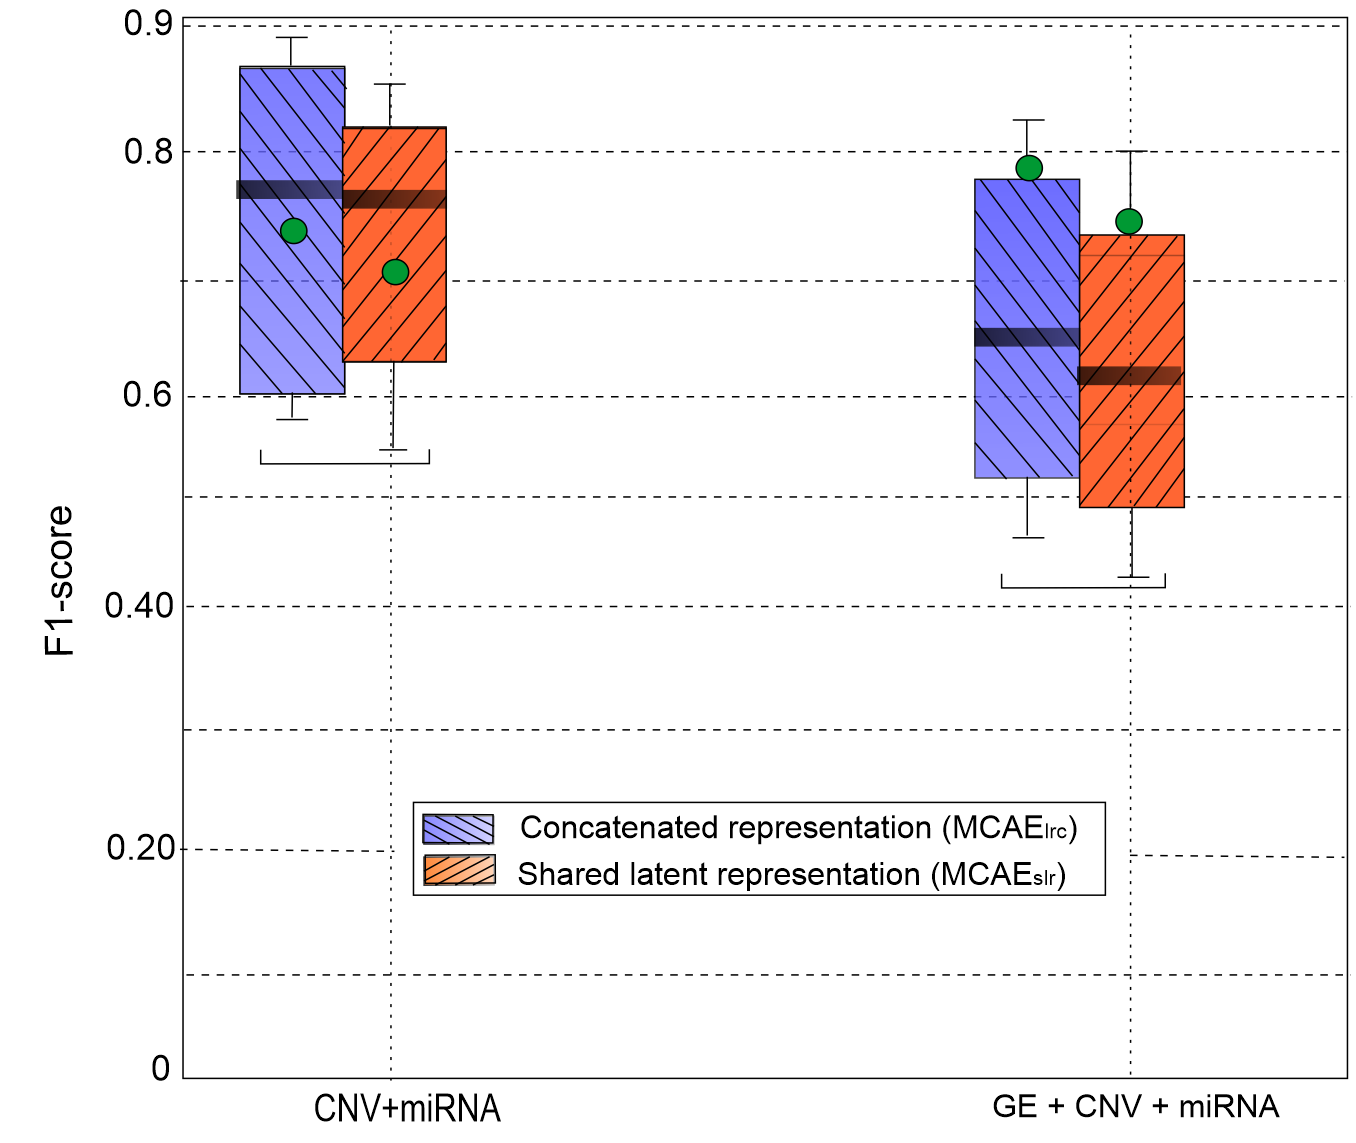
\includegraphics[width=\linewidth,height=55mm]{images/acc_mcae_2.png}
		\caption{CNV+miRNA vs. GE+CNV=miRNA modality}
        \label{fig:ce_ge_cnv_2}
	\end{subfigure}
	\caption{F1 score comparison for $MCAE_{lrc}$ and $MCAE_{slr}$ during supervised finetuning} 
	\label{fig:ce_multimodal_models_2}
\end{figure*}

\hspace*{3.5mm} In particular, the GE+miRNA input combination gave lowest reconstruction errors, whereas GE + CNV + miRNA generates the highest errors so do corresponding f1-scores. Eventually, we found that the ROC curves of the $MCAE_{lrc}$ model show that the AUC scores are consistent across the folds showing stable predictions, giving 4\% boost in AUC scores. This signifies that the predictions by the $MCAE_{lrc}$ model are clearly better than random guessing as well as $MCAE_{slr}$. It also suggests that the predictions made by the $MCAE_{lrc}$ model are strongly correlated with the ground truth, yielding a Pearson product-moment correlation coefficient higher than 0.70 for all the classes. 

\subsubsection{Identification of marker genes}
As it is evident that $MCAE_{lrc}$ classifier outperforms $MCAE_{slr}$, giving better classification accuracy. Therefore, $MCAE_{lrc}$ model is used to score top-k biomarkers. In particular, top genes are identified for which the change in expression values have significant impact on model performance. \Cref{fig:hm_all} shows examples of HM generated for each class across 5 different folds, where each column for one cancer type. As seen, there are similarities across folds and displaying distinct and similar patterns when comparing different cancer types. Red circles highlight similar patterns, e.g., between KIRC and BRCA, and PRAD and LUAD across folds, whereas COAD shows very different patterns. Although there are differences among folds, some patterns are clearly visible. However, intensities did not follow any regular pattern, which signifies that probably Grad-CAM++ or LRP is not suitable for multimodality specific gene ranking. 

\begin{figure*}[h]
    \centering
	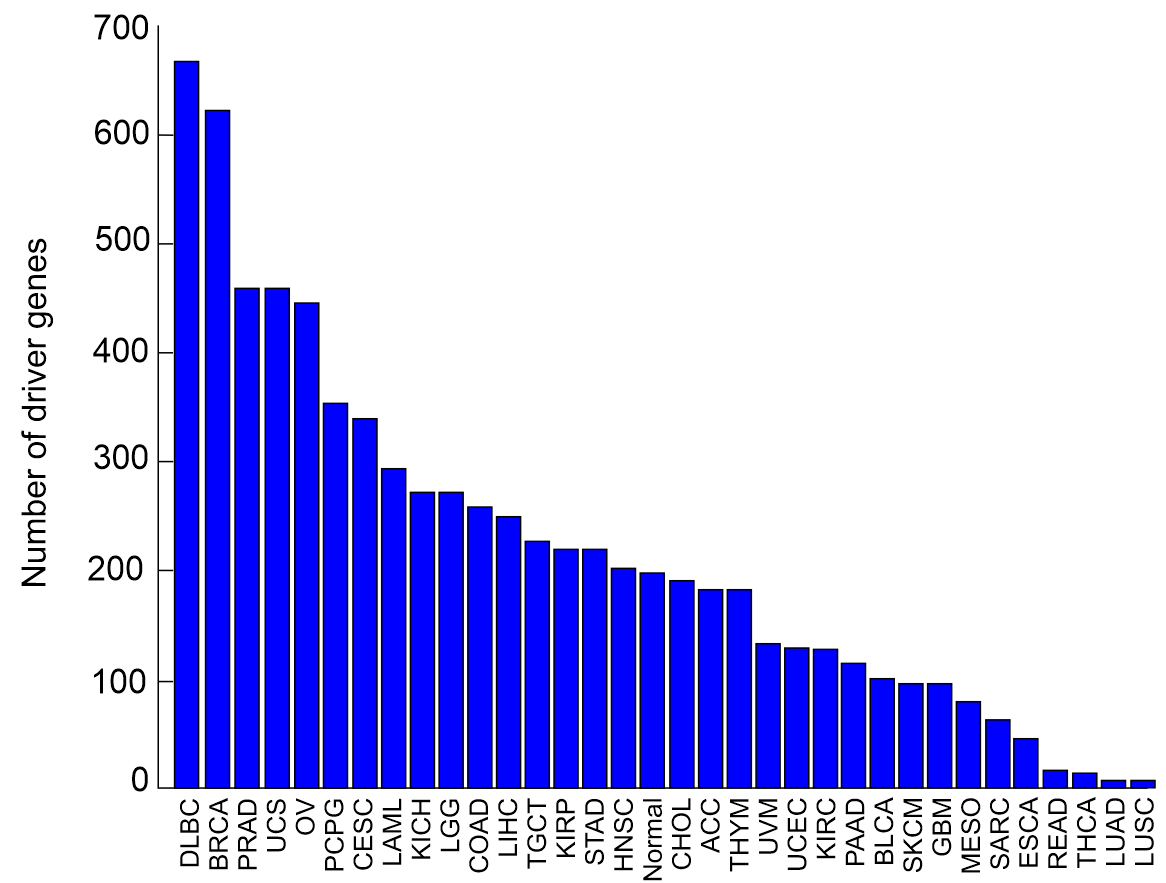
\includegraphics[scale=0.8]{images/driver_genes.png}
	\caption{Identified marker genes, per class with a gene effect score of $\geq$ 0.25}
    \label{fig:dg_cnn}
\end{figure*}

\hspace*{3.5mm} Therefore, global attention mechanism is employed on $MCAE_{lrc}$ model to choose top 660 genes across 33 tumor types as more significant, i.e., top-20 genes per class.
\Cref{fig:dg_cnn} shows the distribution of number of identified marker genes, per class with a gene effect score of $\geq$ 0.25. Since we have more than 20K protein-coding genes, our choice of 660 is still a reasonable choice, as the number of important biomarkers should be small for which even minor changes are sensitive to cancer growth~\cite{zuo2019identification}. All genes in the top-20 list can thus be viewed as tumor-specific biomarkers, which contribute most toward making the predictions. As for other 29 tumor types, only 3 genes qualified in the list. %Further hyperparameter tuning and training of both CNN models might improve this outcome. 
Then for better interpretability, the top-20 list is further narrowed down to top-5, having at least five genes with feature importance of at least 0.25 w.r.t. gene effect score, as shown in \cref{table:proteinimportance_1} and  \cref{table:proteinimportance_2}. % from the 20,500 protein-coding genes. 

\begin{table}
    \caption{Top-5 genes and their importance for cancer types: BRCA, KIRC, LUAD, PRAD, COAD, ACC, BLCA, CESC, CHOL, DLBC, ESCA, GBM, HNSC, KICH, KIRC, and KIRP }
    \label{table:proteinimportance_1} %RF Confusion Matrix Oncogene Subtype
    \begin{center}
    \scriptsize{
    \vspace{-6mm}
    \begin{tabular}{l|l|l|l}
        \toprule
        \textbf{Cohort} & \textbf{Biomarker name} & \textbf{Biomarker type} & \textbf{Importance} \\ 
        \midrule
        \multirow{5}{*}{BRCA} & PIK3CA & Oncogene & 0.78125 \\ %\cline{2-4}
        & TP53 & Protein-coding & 0.760784 \\ %\cline{2-4}
        & GATA3  & Protein-coding & 0.664706 \\ %\cline{2-4}
        & MAP3K1  & Oncogene & 0.574118 \\ %\cline{2-4}
        & APC   & Protein-coding & 0.538039 \\ 
        \midrule
        \multirow{5}{*}{KIRC} & VHL & Oncogene & 0.596078 \\ %\cline{2-4}
        & PBRM1 & Protein-coding  & 0.560784 \\ %\cline{2-4}
        & SETD2 & Protein-coding & 0.540784 \\ %\cline{2-4}
        & PIK3CA & Oncogene & 0.531569 \\ %\cline{2-4}
        & ATM & Oncogene & 0.523137 \\ %\cline{2-4}
        \midrule
        \multirow{5}{*}{LUAD} & KRAS & Oncogene & 0.860000 \\ %\cline{2-4}
        & KEAP1 & Protein-coding & 0.820784 \\ %\cline{2-4}
        & EGFR & Oncogene & 0.764706 \\ %\cline{2-4}
        & TP53 & Protein-coding & 0.674118 \\ %\cline{2-4}
        & MLL3 & Protein-coding & 0.558039 \\ %\cline{2-4}
        \midrule
        \multirow{5}{*}{PRAD}& SPOP & Oncogene & 0.556078 \\ %\cline{2-4}
        & TP53 & Oncogene & 0.520784 \\ %\cline{2-4}
        & MED12 & Protein-coding & 0.510784 \\ %\cline{2-4}
        & PIK3CA & Protein-coding & 0.491569 \\ %\cline{2-4}
        & FOXA1 & Protein-coding & 0.453137 \\ %\cline{2-4}
        \midrule
        \multirow{5}{*}{COAD}& EPHA6 & Protein-coding & 0.756078 \\ %\cline{2-4}
        & TIMP1 & Protein-coding & 0.720784 \\ %\cline{2-4}
        & ART5 & Protein-coding & 0.680784 \\ %\cline{2-4}
        & FOXD1 & Protein-coding & 0.661569 \\ %\cline{2-4}
        & AMBN & Protein-coding & 0.563137 \\ %\cline{2-4}
        \midrule
        \multirow{5}{*}{ACC} & PIK3CA & Oncogene & 0.78125 \\ %\cline{2-4}
        & TP53 & Protein-coding & 0.760784 \\ %\cline{2-4}
        & GATA3  & Protein-coding & 0.664706 \\ %\cline{2-4}
        & MAP3K1  & Oncogene & 0.574118 \\ %\cline{2-4}
        & APC   & Protein-coding & 0.538039 \\ 
        \midrule
        \multirow{5}{*}{BLCA} & VHL & Oncogene & 0.596078 \\ %\cline{2-4}
        & PBRM1 & Protein-coding  & 0.560784 \\ %\cline{2-4}
        & SETD2 & Protein-coding & 0.540784 \\ %\cline{2-4}
        & PIK3CA & Oncogene & 0.531569 \\ %\cline{2-4}
        & ATM & Oncogene & 0.523137 \\ %\cline{2-4}
        \midrule
        \multirow{5}{*}{CESC}& KRAS & Oncogene & 0.860000 \\ %\cline{2-4}
        & KEAP1 & Protein-coding & 0.820784 \\ %\cline{2-4}
        & EGFR & Oncogene & 0.764706 \\ %\cline{2-4}
        & TP53 & Protein-coding & 0.674118 \\ %\cline{2-4}
        & MLL3 & Protein-coding & 0.558039 \\ %\cline{2-4}
        \midrule
        \multirow{5}{*}{CHOL}& SPOP & Oncogene & 0.556078 \\ %\cline{2-4}
        & TP53 & Oncogene & 0.520784 \\ %\cline{2-4}
        & MED12 & Protein-coding & 0.510784 \\ %\cline{2-4}
        & PIK3CA & Protein-coding & 0.491569 \\ %\cline{2-4}
        & FOXA1 & Protein-coding & 0.453137 \\ %\cline{2-4}
        \midrule
        \multirow{5}{*}{DLBC} & PIK3CA & Oncogene & 0.78125 \\ %\cline{2-4}
        & TP53 & Protein-coding & 0.760784 \\ %\cline{2-4}
        & GATA3  & Protein-coding & 0.664706 \\ %\cline{2-4}
        & MAP3K1  & Oncogene & 0.574118 \\ %\cline{2-4}
        & APC   & Protein-coding & 0.538039 \\ 
        \midrule 
        \multirow{5}{*}{ESCA} & VHL & Oncogene & 0.596078 \\ %\cline{2-4}
        & PBRM1 & Protein-coding  & 0.560784 \\ %\cline{2-4}
        & SETD2 & Protein-coding & 0.540784 \\ %\cline{2-4}
        & PIK3CA & Oncogene & 0.531569 \\ %\cline{2-4}
        & ATM & Oncogene & 0.523137 \\ %\cline{2-4}
        \midrule
        \multirow{5}{*}{GBM}& KRAS & Oncogene & 0.860000 \\ %\cline{2-4}
        & KEAP1 & Protein-coding & 0.820784 \\ %\cline{2-4}
        & EGFR & Oncogene & 0.764706 \\ %\cline{2-4}
        & TP53 & Protein-coding & 0.674118 \\ %\cline{2-4}
        & MLL3 & Protein-coding & 0.558039 \\ %\cline{2-4}
        \midrule
        \multirow{5}{*}{HNSC}& SPOP & Oncogene & 0.556078 \\ %\cline{2-4}
        & TP53 & Oncogene & 0.520784 \\ %\cline{2-4}
        & MED12 & Protein-coding & 0.510784 \\ %\cline{2-4}
        & PIK3CA & Protein-coding & 0.491569 \\ %\cline{2-4}
        & FOXA1 & Protein-coding & 0.453137 \\ %\cline{2-4}
        \midrule
        \multirow{5}{*}{KICH}& EPHA6 & Protein-coding & 0.756078 \\ %\cline{2-4}
        & TIMP1 & Protein-coding & 0.720784 \\ %\cline{2-4}
        & ART5 & Protein-coding & 0.680784 \\ %\cline{2-4}
        & FOXD1 & Protein-coding & 0.661569 \\ %\cline{2-4}
        & AMBN & Protein-coding & 0.563137 \\ %\cline{2-4}
        \midrule
        \multirow{5}{*}{KIRC}& EPHA6 & Protein-coding & 0.756078 \\ %\cline{2-4}
        & TIMP1 & Protein-coding & 0.720784 \\ %\cline{2-4}
        & ART5 & Protein-coding & 0.680784 \\ %\cline{2-4}
        & FOXD1 & Protein-coding & 0.661569 \\ %\cline{2-4}
        & AMBN & Protein-coding & 0.563137 \\ %\cline{2-4}
        \midrule
        \multirow{5}{*}{KIRP}& EPHA6 & Protein-coding & 0.756078 \\ %\cline{2-4}
        & TIMP1 & Protein-coding & 0.720784 \\ %\cline{2-4}
        & ART5 & Protein-coding & 0.680784 \\ %\cline{2-4}
        & FOXD1 & Protein-coding & 0.661569 \\ %\cline{2-4}
        & AMBN & Protein-coding & 0.563137 \\ %\cline{2-4}
        \midrule
        \bottomrule
        \end{tabular}}
        \vspace{-4mm}
    \end{center}
\end{table}

\begin{table}
    \caption{Top-5 genes and their importance for cancer types: LAML, LGG, LIHC, LUSC, MESO, OV, PAAD, PCPG, READ, SARC, SKCM, STAD, TGCT, THCA, THYM, UCS and UVM}
    \label{table:proteinimportance_2} %RF Confusion Matrix Oncogene Subtype
    \begin{center}
    \scriptsize{
    \vspace{-6mm}
    \begin{tabular}{l|l|l|l}
        \toprule
        \textbf{Cohort} & \textbf{Biomarker name} & \textbf{Biomarker type} & \textbf{Importance} \\ 
        \midrule
        \multirow{5}{*}{LAML} & VHL & Oncogene & 0.596078 \\ %\cline{2-4}
        & PBRM1 & Protein-coding  & 0.560784 \\ %\cline{2-4}
        & SETD2 & Protein-coding & 0.540784 \\ %\cline{2-4}
        & PIK3CA & Oncogene & 0.531569 \\ %\cline{2-4}
        & ATM & Oncogene & 0.523137 \\ %\cline{2-4}
        \midrule
        \multirow{5}{*}{LGG}& KRAS & Oncogene & 0.860000 \\ %\cline{2-4}
        & KEAP1 & Protein-coding & 0.820784 \\ %\cline{2-4}
        & EGFR & Oncogene & 0.764706 \\ %\cline{2-4}
        & TP53 & Protein-coding & 0.674118 \\ %\cline{2-4}
        & MLL3 & Protein-coding & 0.558039 \\ %\cline{2-4}
        \midrule
        \multirow{5}{*}{LIHC}& SPOP & Oncogene & 0.556078 \\ %\cline{2-4}
        & TP53 & Oncogene & 0.520784 \\ %\cline{2-4}
        & MED12 & Protein-coding & 0.510784 \\ %\cline{2-4}
        & PIK3CA & Protein-coding & 0.491569 \\ %\cline{2-4}
        & FOXA1 & Protein-coding & 0.453137 \\ %\cline{2-4}
        \midrule
        \multirow{5}{*}{LUSC}& EPHA6 & Protein-coding & 0.756078 \\ %\cline{2-4}
        & TIMP1 & Protein-coding & 0.720784 \\ %\cline{2-4}
        & ART5 & Protein-coding & 0.680784 \\ %\cline{2-4}
        & FOXD1 & Protein-coding & 0.661569 \\ %\cline{2-4}
        & AMBN & Protein-coding & 0.563137 \\ %\cline{2-4}
        \midrule
        \multirow{5}{*}{MESO} & PIK3CA & Oncogene & 0.78125 \\ %\cline{2-4}
        & TP53 & Protein-coding & 0.760784 \\ %\cline{2-4}
        & GATA3  & Protein-coding & 0.664706 \\ %\cline{2-4}
        & MAP3K1  & Oncogene & 0.574118 \\ %\cline{2-4}
        & APC   & Protein-coding & 0.538039 \\ 
        \midrule
        \multirow{5}{*}{OV} & VHL & Oncogene & 0.596078 \\ %\cline{2-4}
        & PBRM1 & Protein-coding  & 0.560784 \\ %\cline{2-4}
        & SETD2 & Protein-coding & 0.540784 \\ %\cline{2-4}
        & PIK3CA & Oncogene & 0.531569 \\ %\cline{2-4}
        & ATM & Oncogene & 0.523137 \\ %\cline{2-4}
        \midrule
        \multirow{5}{*}{PAAD}& KRAS & Oncogene & 0.860000 \\ %\cline{2-4}
        & KEAP1 & Protein-coding & 0.820784 \\ %\cline{2-4}
        & EGFR & Oncogene & 0.764706 \\ %\cline{2-4}
        & TP53 & Protein-coding & 0.674118 \\ %\cline{2-4}
        & MLL3 & Protein-coding & 0.558039 \\ %\cline{2-4}
        \midrule
        \multirow{5}{*}{PCPG}& SPOP & Oncogene & 0.556078 \\ %\cline{2-4}
        & TP53 & Oncogene & 0.520784 \\ %\cline{2-4}
        & MED12 & Protein-coding & 0.510784 \\ %\cline{2-4}
        & PIK3CA & Protein-coding & 0.491569 \\ %\cline{2-4}
        & FOXA1 & Protein-coding & 0.453137 \\ %\cline{2-4}
        \midrule 
        \multirow{5}{*}{READ}& EPHA6 & Protein-coding & 0.756078 \\ %\cline{2-4}
        & TIMP1 & Protein-coding & 0.720784 \\ %\cline{2-4}
        & ART5 & Protein-coding & 0.680784 \\ %\cline{2-4}
        & FOXD1 & Protein-coding & 0.661569 \\ %\cline{2-4}
        & AMBN & Protein-coding & 0.563137 \\ %\cline{2-4}
        \midrule
        \multirow{5}{*}{SARC} & PIK3CA & Oncogene & 0.78125 \\ %\cline{2-4}
        & TP53 & Protein-coding & 0.760784 \\ %\cline{2-4}
        & GATA3  & Protein-coding & 0.664706 \\ %\cline{2-4}
        & MAP3K1  & Oncogene & 0.574118 \\ %\cline{2-4}
        & APC   & Protein-coding & 0.538039 \\ 
        \midrule
        \multirow{5}{*}{SKCM} & VHL & Oncogene & 0.596078 \\ %\cline{2-4}
        & PBRM1 & Protein-coding  & 0.560784 \\ %\cline{2-4}
        & SETD2 & Protein-coding & 0.540784 \\ %\cline{2-4}
        & PIK3CA & Oncogene & 0.531569 \\ %\cline{2-4}
        & ATM & Oncogene & 0.523137 \\ %\cline{2-4}
        \midrule
        \multirow{5}{*}{STAD}& KRAS & Oncogene & 0.860000 \\ %\cline{2-4}
        & KEAP1 & Protein-coding & 0.820784 \\ %\cline{2-4}
        & EGFR & Oncogene & 0.764706 \\ %\cline{2-4}
        & TP53 & Protein-coding & 0.674118 \\ %\cline{2-4}
        & MLL3 & Protein-coding & 0.558039 \\ %\cline{2-4}
        \midrule
        \multirow{5}{*}{TGCT}& SPOP & Oncogene & 0.556078 \\ %\cline{2-4}
        & TP53 & Oncogene & 0.520784 \\ %\cline{2-4}
        & MED12 & Protein-coding & 0.510784 \\ %\cline{2-4}
        & PIK3CA & Protein-coding & 0.491569 \\ %\cline{2-4}
        & FOXA1 & Protein-coding & 0.453137 \\ %\cline{2-4}
        \midrule
        \multirow{5}{*}{THCA}& EPHA6 & Protein-coding & 0.756078 \\ %\cline{2-4}
        & TIMP1 & Protein-coding & 0.720784 \\ %\cline{2-4}
        & ART5 & Protein-coding & 0.680784 \\ %\cline{2-4}
        & FOXD1 & Protein-coding & 0.661569 \\ %\cline{2-4}
        & AMBN & Protein-coding & 0.563137 \\ %\cline{2-4}
        \midrule
        \multirow{5}{*}{THYM}& EPHA6 & Protein-coding & 0.756078 \\ %\cline{2-4}
        & TIMP1 & Protein-coding & 0.720784 \\ %\cline{2-4}
        & ART5 & Protein-coding & 0.680784 \\ %\cline{2-4}
        & FOXD1 & Protein-coding & 0.661569 \\ %\cline{2-4}
        & AMBN & Protein-coding & 0.563137 \\ %\cline{2-4}
        \midrule
        \multirow{5}{*}{UCS}& EPHA6 & Protein-coding & 0.756078 \\ %\cline{2-4}
        & TIMP1 & Protein-coding & 0.720784 \\ %\cline{2-4}
        & ART5 & Protein-coding & 0.680784 \\ %\cline{2-4}
        & FOXD1 & Protein-coding & 0.661569 \\ %\cline{2-4}
        & AMBN & Protein-coding & 0.563137 \\ %\cline{2-4}
        \midrule
        \multirow{5}{*}{UVM} & PIK3CA & Oncogene & 0.78125 \\ %\cline{2-4}
        & TP53 & Protein-coding & 0.760784 \\ %\cline{2-4}
        & GATA3  & Protein-coding & 0.664706 \\ %\cline{2-4}
        & MAP3K1  & Oncogene & 0.574118 \\ %\cline{2-4}
        & APC  & Protein-coding & 0.538039 \\ 
        %\bottomrule
        \end{tabular}}
        \vspace{-4mm}
    \end{center}
\end{table}

\subsection{Statistical validation of top biomarkers}
To validate the findings, both saturation and pathway enrichment analyses are carried out for the identified genes. For the 32 tumor types, except for COAD, the saturation is obtained from TumorPortal\footnote{ \url{http://www.tumorportal.org/}}~\cite{lawrence2014discovery}. The proposed approach makes some false predictions. In particular, 550 out of 660 genes are found to be associated with corresponding cancer types, making only 25 false identifications. Considering, such a high-dimensional feature space, 86\% accurate identification is still moderately high.
Validation for the COAD cancer follows a signature-based approach\footnote{It was originally used for predicting the progression of colorectal cancer}~\cite{zuo2019identification}. On the other hand, inspired by the pathway association experiment used in literature~\cite{lyu2018deep} and to find out the relations between these pathways and tumor types, KEGG pathway analysis results for top 20 genes for each cancer type are obtained from the TumorPortal and David web site. 
%Further, we did a literature review on the results trying to find out the relations between these pathways and tumor types. 
Related pathways with p-value smaller than 0.005 are only considered. Lyu et al.~\cite{lyu2018deep} found top 660 genes to have significant enrichment of pathways, covering 24 tumor types. According to their study, 16 tumor types have at least one related pathway. As suggested, related genes in these pathways can be viewed as tumor specific biomarkers~\cite{lyu2018deep}. 

\begin{sidewaysfigure*}
\centering
	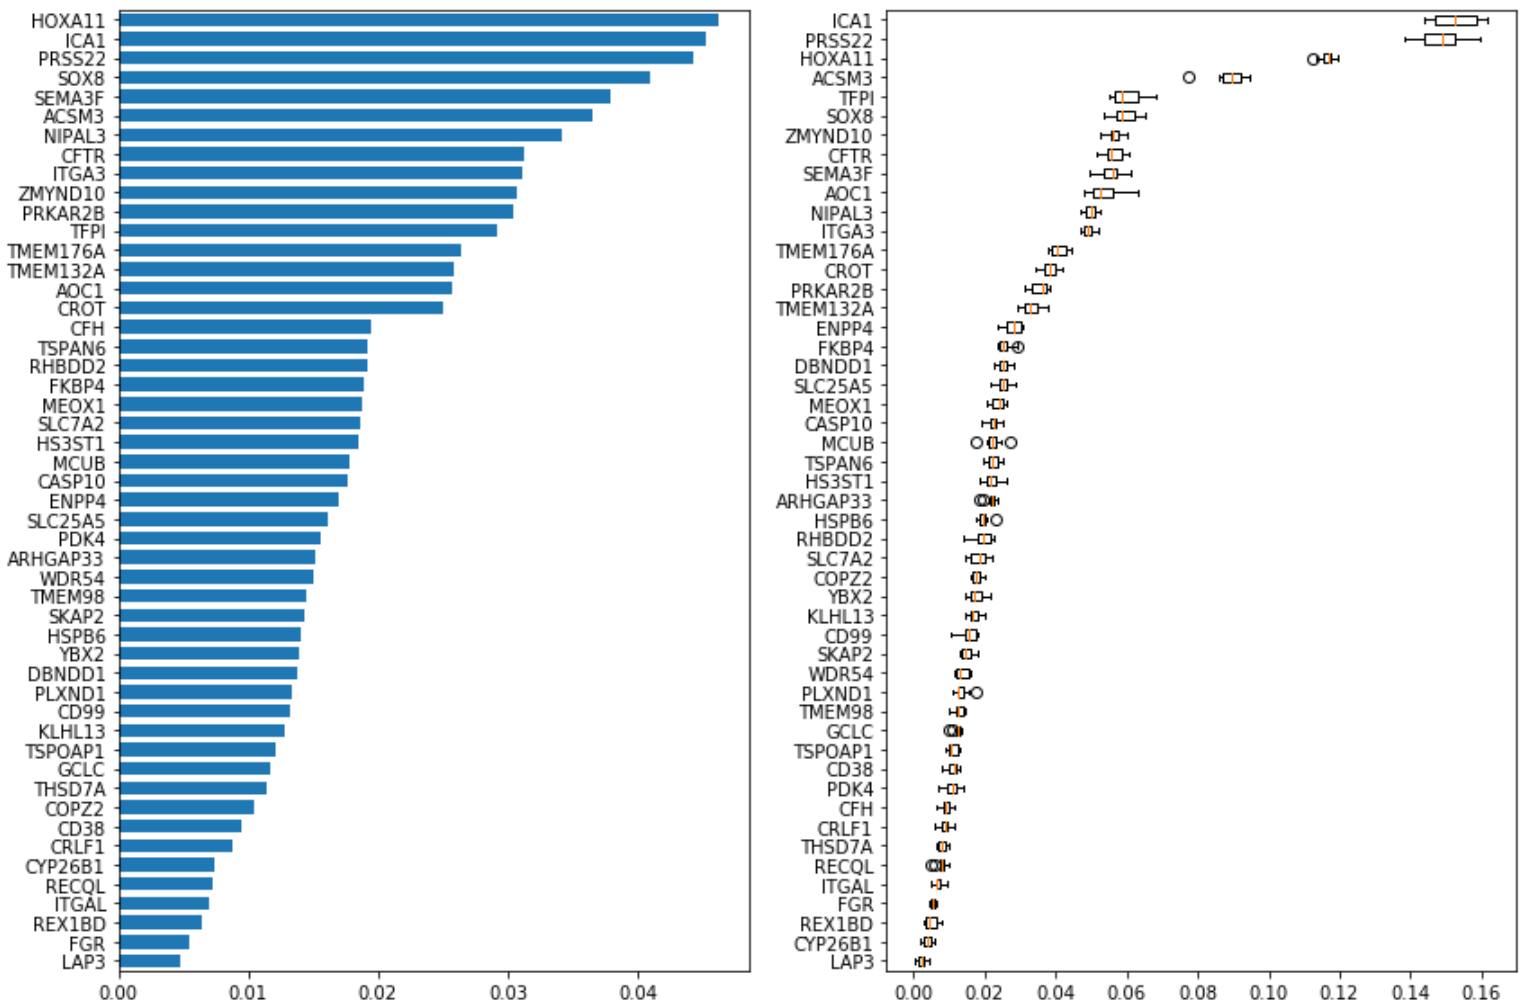
\includegraphics[scale=1.0]{images/rf_fi.png}
	\caption[Interpretation of marker genes]{Interpretation of marker genes per class with a gene effect score of minimum 0.25. Left: random forest-based permutation feature importance, right: $MCAE_{lrc}$ model-based feature importance. Genes and importance score are shown on y and x axis, respectively. }
    \label{fig:pfi}
\end{sidewaysfigure*}

\hspace*{3.5mm} For the remaining, 8 tumor types, two significant enriched concurrent pathways are found, which are \texttt{hsa04512}: ECM-receptor interaction and \texttt{hsa04510}: focal adhesion~\cite{lyu2018deep}. Although, no direct related pathways are found~\cite{lyu2018deep}. 
%However, the related genes are not the same as to different tumor types. 
For the BRCA cancer type, they observed that SDC1, COL4A1, COL3A1, COL6A3, COL1A2, ITGA11, COL6A2, COL6A1, COL1A1, COL5A2, and FN1 are ECM-receptor interaction pathway related genes~\cite{lyu2018deep}. For the ESCA cancer type, VWF, ITGA6, LAMC3, ITGAV, TNC, ITGB6, ITGB4, ITGA3, COL1A1, COL5A2, and COL4A6 are found to be related genes~\cite{lyu2018deep}. Similarly,  CAV1, TNC, COL3A1, PIK3CD, ITGA3, ITGB3, COL5A3, CCND1, LAMB2, FYN, COMP, COL6A3, COL6A2, COL6A1, COL1A1, LAMB1, PARVB, SPP1, FN1, and SHC4 are the related top genes for SKCM cancer type w.r.t focal adhesion pathway~\cite{lyu2018deep}. For the THCA cancer type, COL4A4, COL4A3, CAV2, CAV1, PGF, BCAR1, MET, IGF1, ITGA3, LAMA5, COL1A2, LAMC2, COL1A1, and FN1 are related top genes. These sets are not quite the same in different tumor types, which shows that they can be potential biomarkers~\cite{lyu2018deep}. However, no significant enriched pathways were found for the CHOL, COAD, READ, GBM, KICH, LGG, LUSC, OV, and UVM tumor types~\cite{lyu2018deep}. 

%However, the approach based on global attention mechanigm, 
%The samples for CHOL and KICH are very limited, hence these were omitted for the pathway enrichment calculation. Further, since the classification accuracy for READ tumor type is very low, it is omitted as well. With respect to the 6 remaining tumor types, the query size is reduced from top-20 to top-5. For the COAD tumor type, the top-1 gene LGALS4 is a protein coding gene. %The expression of this gene is restricted to small intestine, colon, and rectum, and it is under-expressed in colorectal cancer. 

%\hspace*{3.5mm} For the GBM cancer type, top-1 gene found to be a protein coding gene named GFAP\footnote{GFAP gene encodes one of the major intermediate filament proteins of mature astrocytes, which is used as a marker to distinguish astrocytes from other glial cells during development in the brain region}. LGG (Brain Lower Grade Glioma) is also a tumor in the brain, its top 1-4 genes are all pseudo-genes, while the top5 gene GFAP is the gene related to brain. As to LUSC (Lung squamous cell carcinoma), its top1 gene SFTPA2 has been implicated in many lung diseases~\cite{lyu2018deep}. As to OV~(Ovarian cancer)~\cite{lyu2018deep}, its top-1 gene MUC16~(CA125) was said to be the only reliable diagnostic marker for ovarian cancer. As to UVM~(Uveal Melanoma), its top1 gene CD44 were tested to be strongly expressed in several cell lines of human uveal melanoma~\cite{lyu2018deep}. All the above results have shown the top genes have very close relations to the corresponding tumor types, which could be viewed as potential biomarkers.

\subsection{Global explanations}
In order to explain global explainability of the trained models, we first analyse both global feature importance and interactions. While feature importance assign a score to input features based on how useful they are at predicting a target variable, feature impact identifies which features in a dataset have the greatest positive or negative effect on the outcomes of the model. Global feature importance helps identify which features in the dataset have the greatest effect on the outcomes of the model. %On the other hand, feature impact identifies which features in a dataset have the greatest positive or negative effect on the outcomes of the model. 

\subsubsection{Global feature importance}
Identification all significant common genes help understand various aspects for a specific cancer type~(e.g., BRCA carcinogenesis). These top genes have close relations to the corresponding tumor types, which could be viewed as potential biomarkers. \Cref{fig:comgenes} shows top-10 common driver genes across 33 cancer types based on gene expression with Grad-CAM++ and LRP. As shown, TP53, GATA3, EGFR, ATM, MLL3, MTOR, MPO, FOXD1, MED12, and GATA3 genes are identified as common driver genes across cancer types with Grad-CAM++, where TP53 protein-coding gene has the highest feature importance of 0.75. On the other hand, TP53, EGFR, AMBN, SETD2, MPO, MTOR, FOXD1, GATA3, and MED12 genes are identified as common driver genes across cancer types with LRP, with the TP53 protein-coding gene having the highest feature importance of 0.78. 
%with $MCAE_{lrc}$ model

\begin{figure*}
	\centering
	\begin{subfigure}{.48\linewidth}
		\centering
		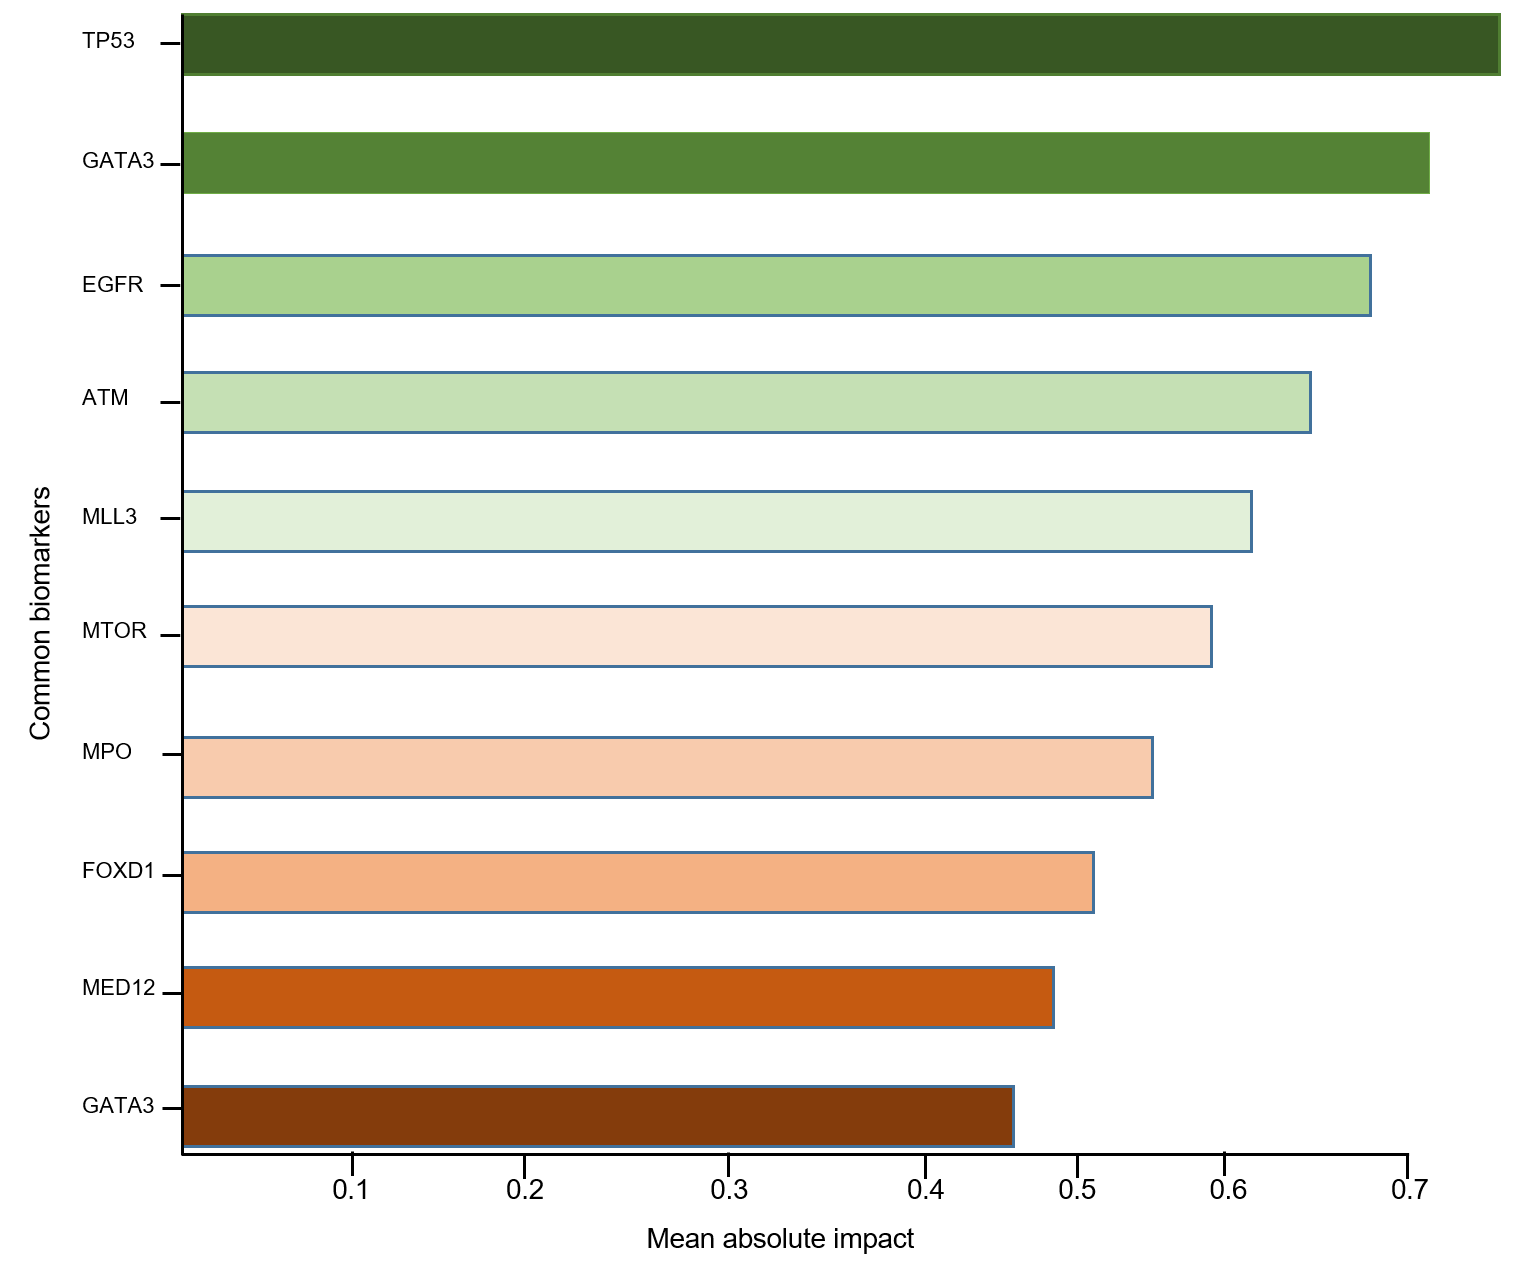
\includegraphics[scale=0.4]{images/gcam_fi.png}
		\caption{Grad-CAM++}
        \label{fig:comgenegcam}
	\end{subfigure}
	\begin{subfigure}{0.48\linewidth}
		\centering
		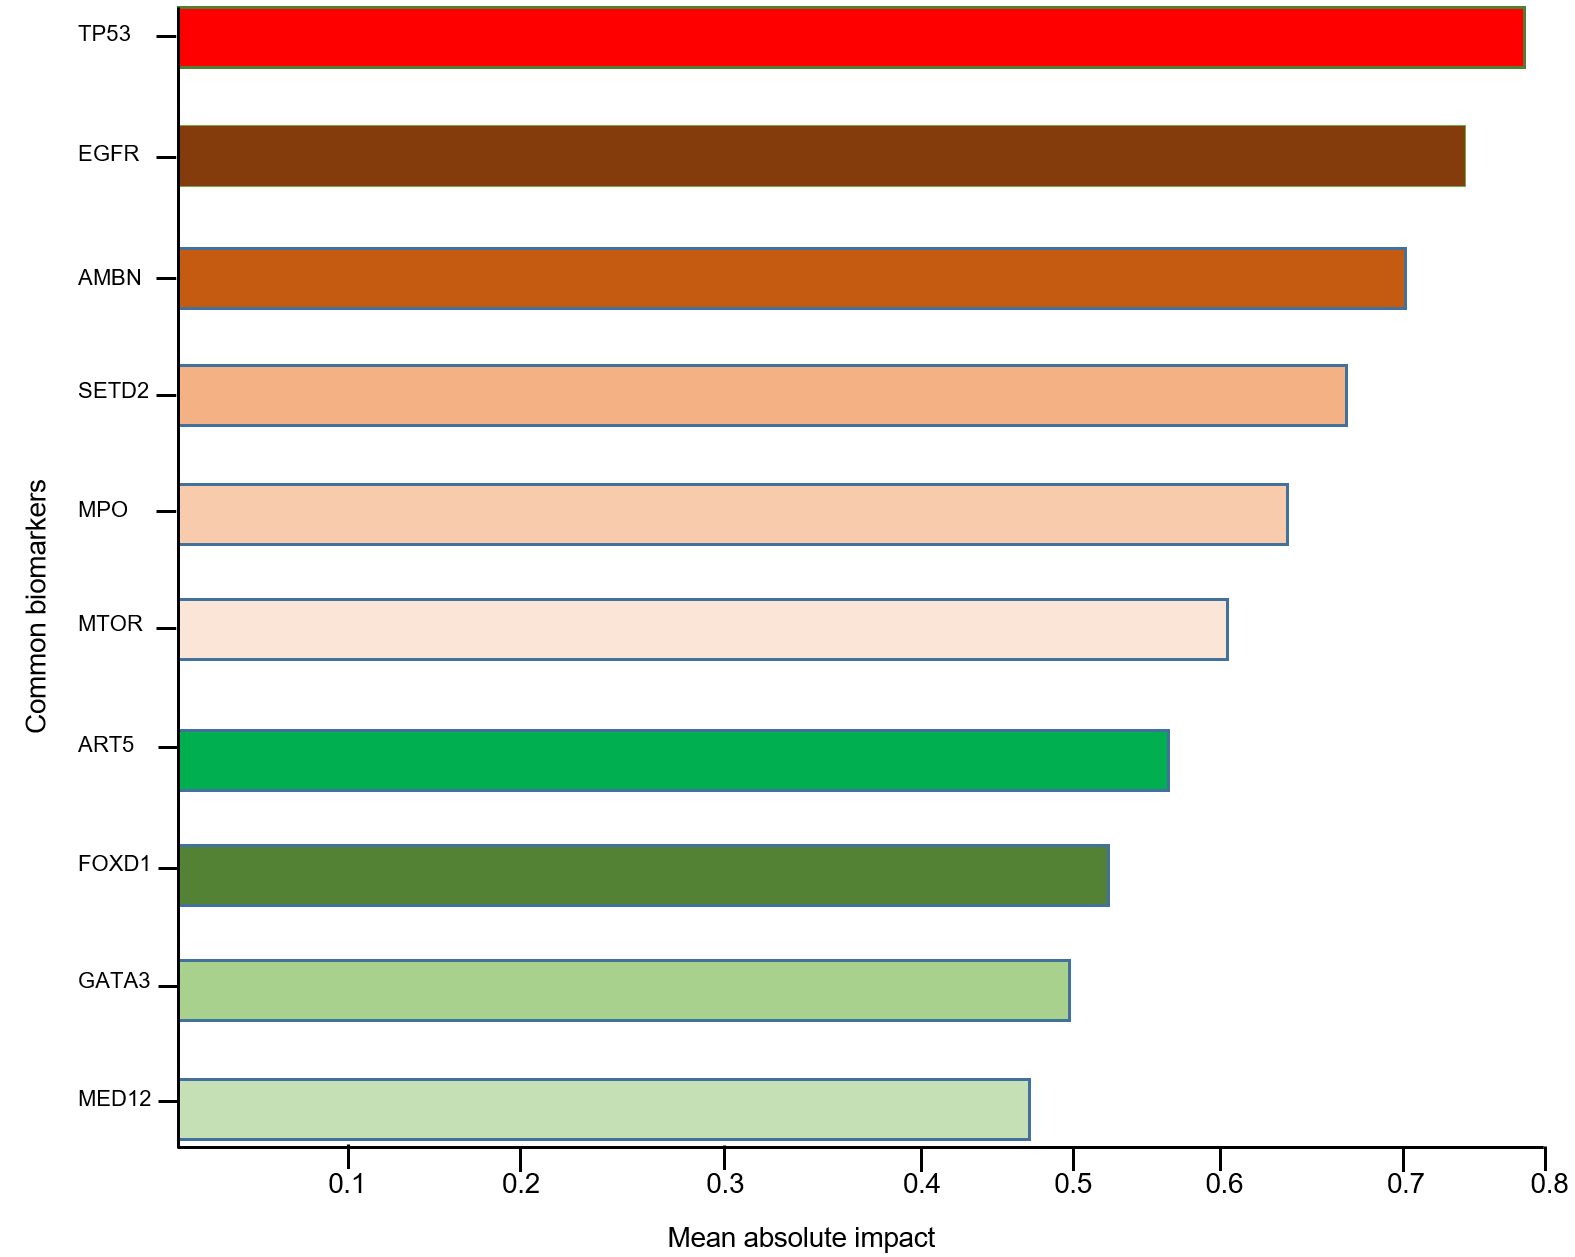
\includegraphics[scale=0.4]{images/lrp_fi.png}
		\caption{LRP}
        \label{fig:comgeneglrp}
	\end{subfigure}
	\caption{Common driver genes across 33 cancer types based on gene expression profiles} 
	\label{fig:comgenes}
\end{figure*}

%\subsubsection{Global feature importance}
\hspace*{3.5mm} Globally important features identified with attention mechanism are shown in \cref{fig:global_feature_importance}. Then, based on the identified features, a score is assigned to input features based on how useful they are at predicting a target variable for the $MCAE_{lrc}$ model. The graph in \cref{fig:global_feature_importance} signifies that BNC1, GBP4, and TFAP2A are the top-3 most important variables according to the $MCAE_{lrc}$ model. Since each variable might affect the outcome differently, exploring other features can provide how each variable could impact the outcome. On average, gene BNC1 will change the model outcome by 0.1. 

\iffalse
\begin{sidewaysfigure*}
	\centering
	\begin{subfigure}{.48\linewidth}
		\centering
		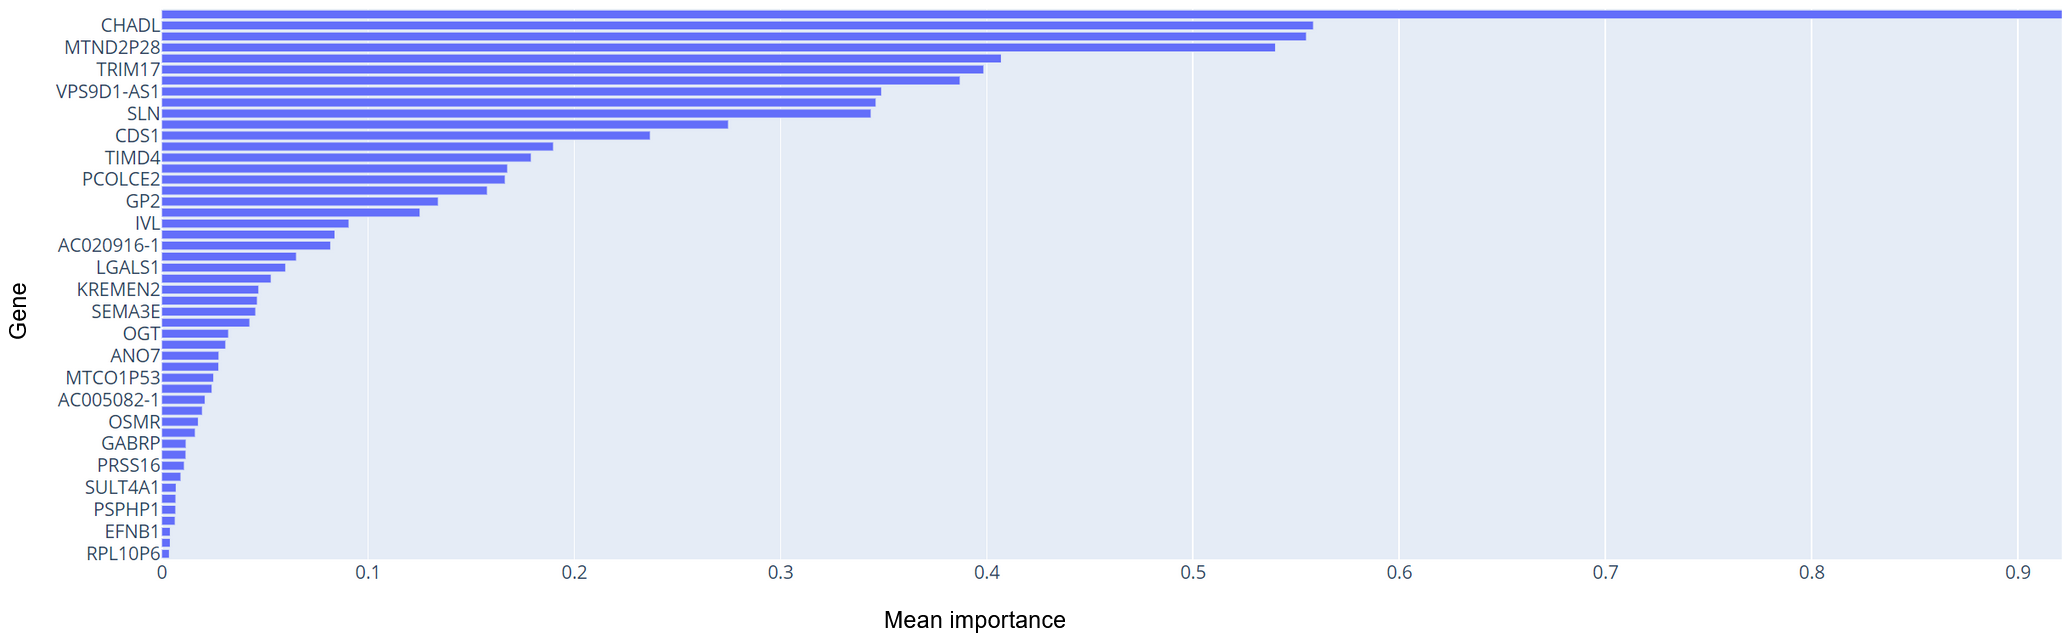
\includegraphics[scale=0.65]{images/global_fi_1.png}
		\caption{Global feature importance}
        \label{fig:global_feature_importance}
	\end{subfigure}
	\begin{subfigure}{0.48\linewidth}
		\centering
		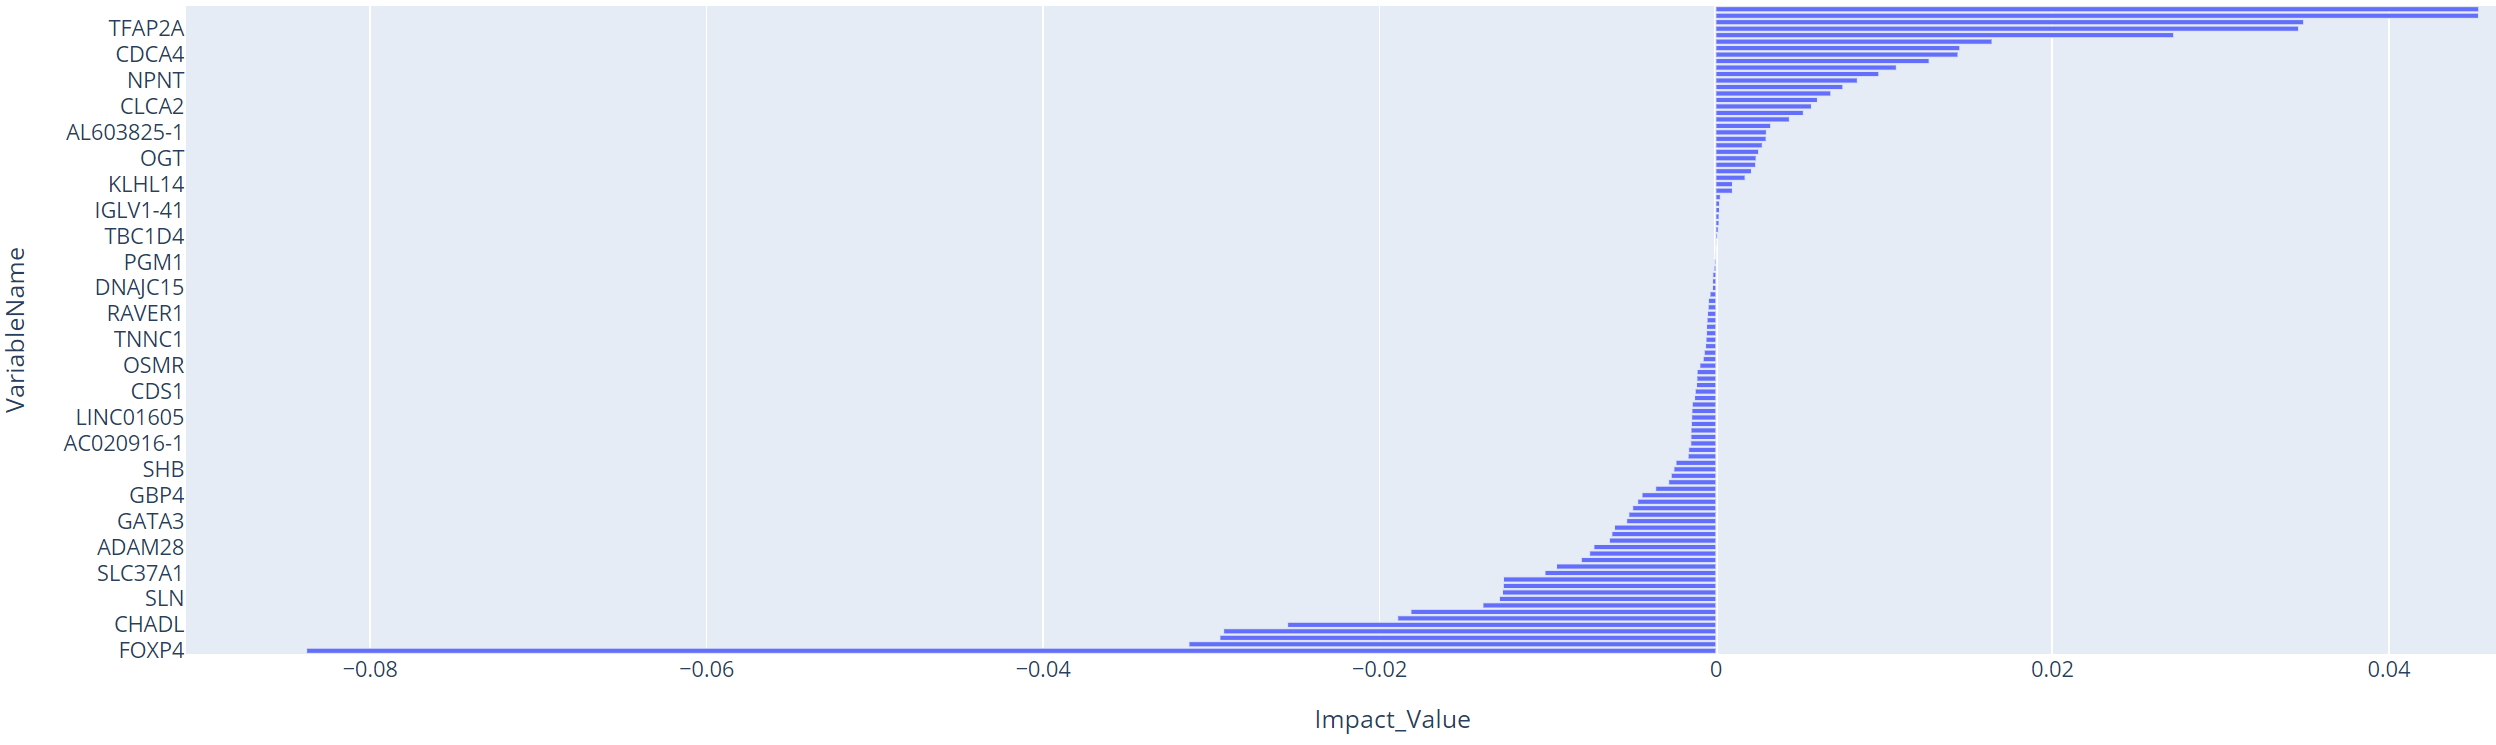
\includegraphics[scale=0.65]{images/global_fi_2.png}
		\caption{Global feature impacts}
        \label{fig:global_feature_impacts}
	\end{subfigure}
	\caption{Global feature importance and impacts} 
	\label{fig:global_feature_imp_impacts}
\end{sidewaysfigure*}
\fi 

\begin{sidewaysfigure*}
    \centering
	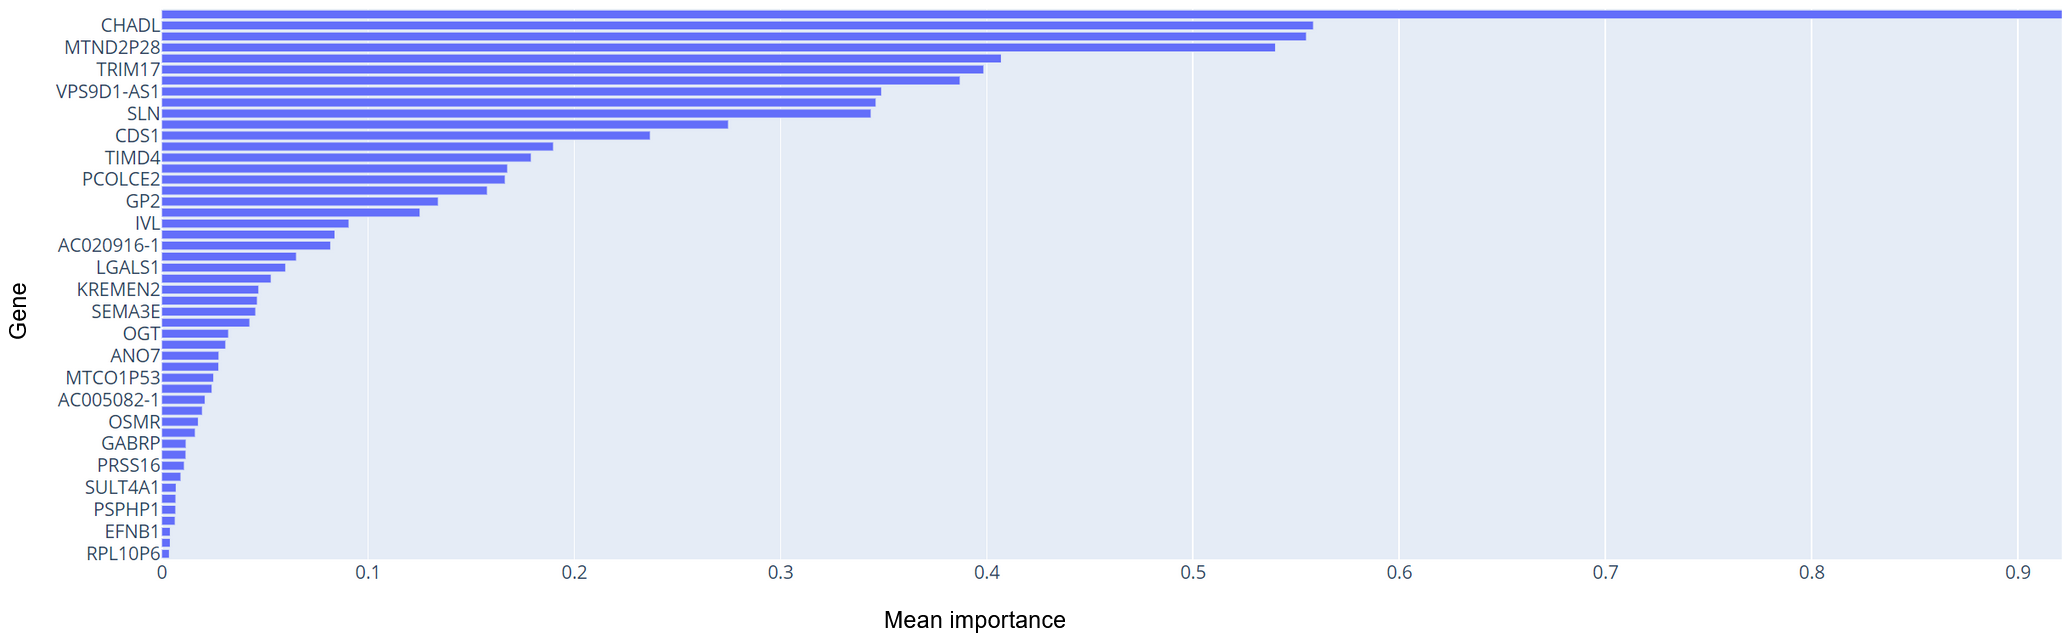
\includegraphics[scale=0.9]{images/global_fi_1.png}
	\caption{Global feature importance}
    \label{fig:global_feature_importance}
\end{sidewaysfigure*}

\begin{sidewaysfigure*}
    \centering
	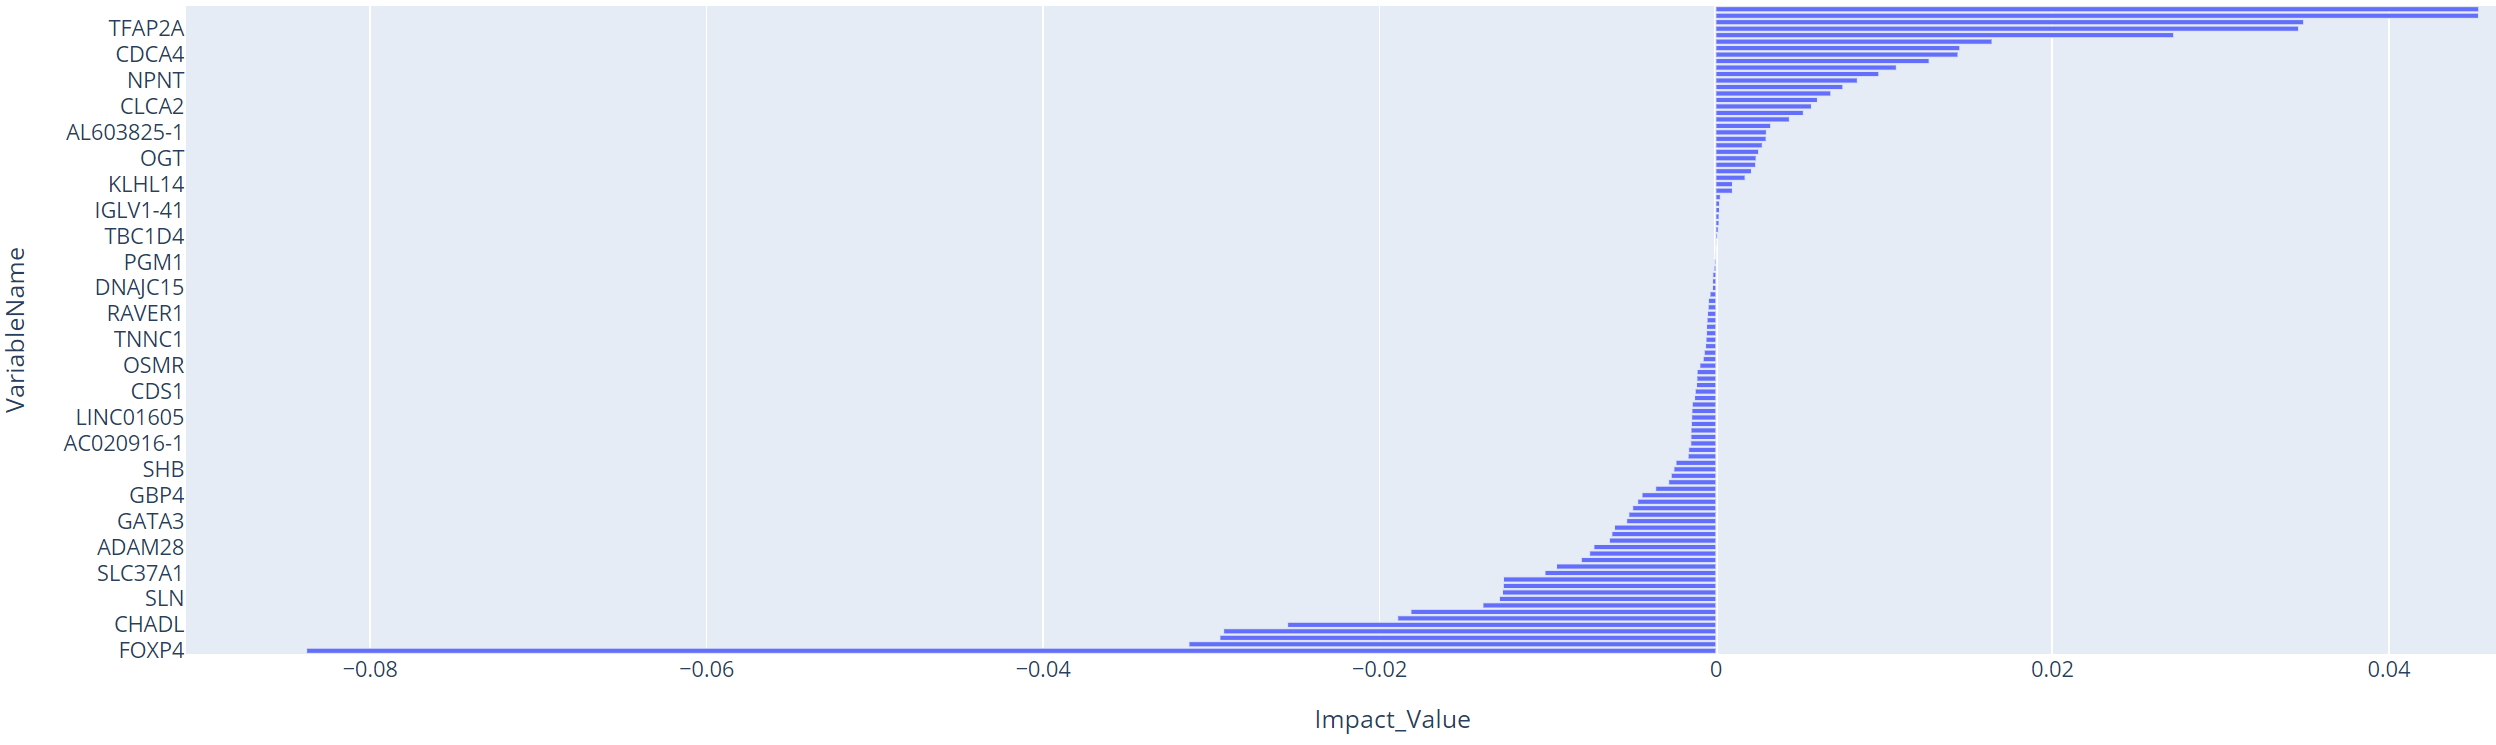
\includegraphics[scale=0.9]{images/global_fi_2.png}
	\caption{Global feature impacts}
    \label{fig:global_feature_impacts}
\end{sidewaysfigure*}

\subsubsection{Global feature impacts}
Feature interactions among globally important features with attention mechanism are demonstrated in \cref{fig:global_feature_impacts}. Global feature impacts signify which features have positive and negative impact on the output of the diagnosis decision. GBP4, VPS9D1-AS1, SLN, SEMA3E, GP2, CXCL10, RAVER1, AL603825-1, TBC1D4, CLTRN, OASL, CWH43, and GABRP positively impact the prediction. This also signifies that if the prediction is in favour of specific cancer type~(let's say COAD) for a specific patient, these variables will play crucial role in maintaining this prediction. However, TRIM17, CDS1, PCOLCE2, MGP, MTCO1P53, TFF3, AC026403-1, HAGLROS, LAPTM5, SULT4A1, EN1, and EFNB1 have negative impact on the prediction. This means that if the prediction is "COAD" and the value of these variables are increased, the final prediction is likely end up flipping-up to another cancer type.

\begin{sidewaysfigure*}
    \centering
	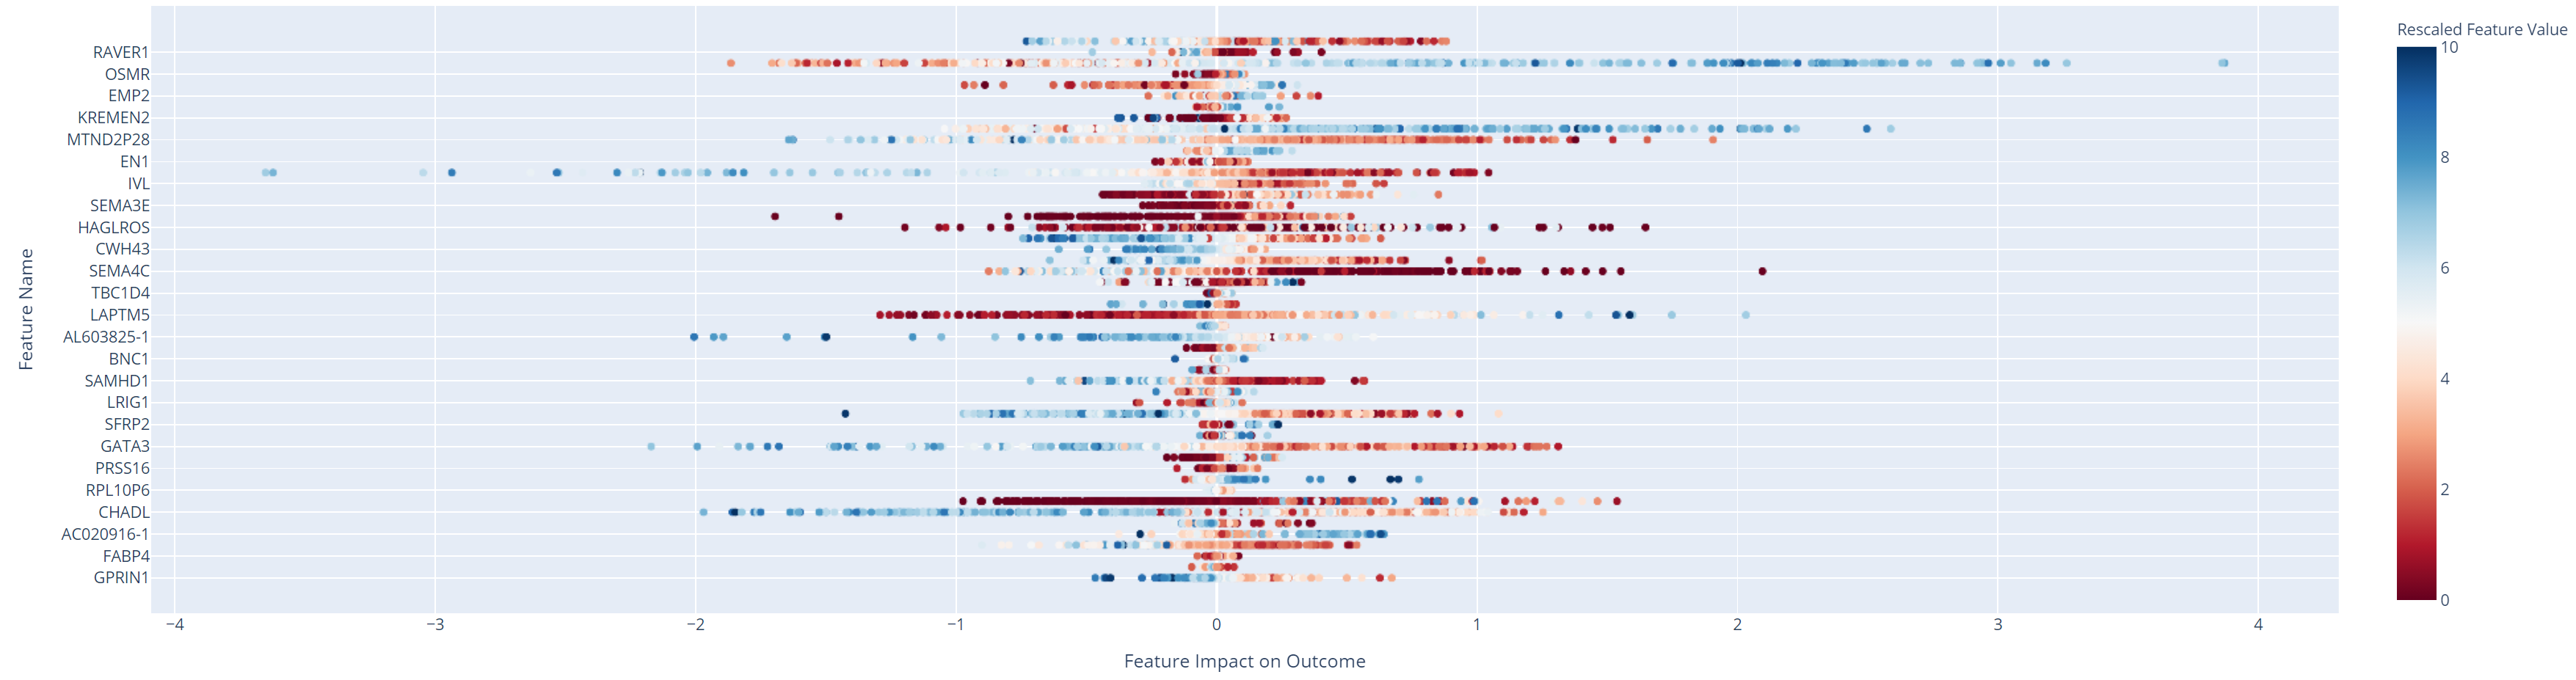
\includegraphics[scale=0.6]{images/summary_plot.png}
	\caption{Summary plot, indicating relationship between feature values and their impacts on models' predictions}
    \label{fig:local_feature_impacts5}
\end{sidewaysfigure*}

\hspace*{3.5mm} Zooming on the individual features provide further insights: it is observed that the average outcome predicted by the model is 9.754495. On average, the variable GBP4, VPS9D1-AS1, and SLN will increase the average model outcome~(9.754495) by 0.04, 0.05, and 0.06, respectively. On the other hand, the variable TRIM17, CDS1, and PCOLCE2 will change the average model outcome~(9.754495) by -0.04, -0.03, and -0.04, respectively. On the other hand, the summary plot by combining feature importance with feature effects are shown in \cref{fig:local_feature_impacts5}. Each point on the summary plot is an impact value for a feature and an instance. The plot indicates the relationship between the value of a feature and the impact on the prediction made by the for the $MCAE_{lrc}$ model. As shown, GPRIN1, FABP4, AC020916-1, CHADL, RPL10P6, PRSS16, GATA3, SFRP2, LRIG1, SAMHD1, BNC1, AL603825-1, LAPTM5, TBC1D4, SEMA4C, CWH43, HAGLROS, SEMA3E, IVL, EN1, MTND2P28, KREMEN2, EMP2, OSMR, and RAVER1 have the highest impact on the model. 


\hspace*{3.5mm} Recently Matej et al.~\cite{vskrlj2020feature} have proposed self-attention networks~(SANs) for identifying feature importance from high-dimensional tabular data. As computing individual feature contributions from the concatenated feature vectors is challenging, the global attention-based feature computation is extended for the MCAE architecture. Through a set of comprehensive experiments they have showed that SAN is very effective on biological data having a large number of features. It is found that attention mechanism can detects larger subsets of features that can improve the performance even liner ML model such as logistic regression. On the contrary, performance of SAN degrades in case of smaller data sets, indicating that having not enough data can distill the relevant parts of the feature space. However, it is yet not clear how the attention concept can be used for computing feature importance in multimodal input setting.

\begin{figure*}
    \centering
	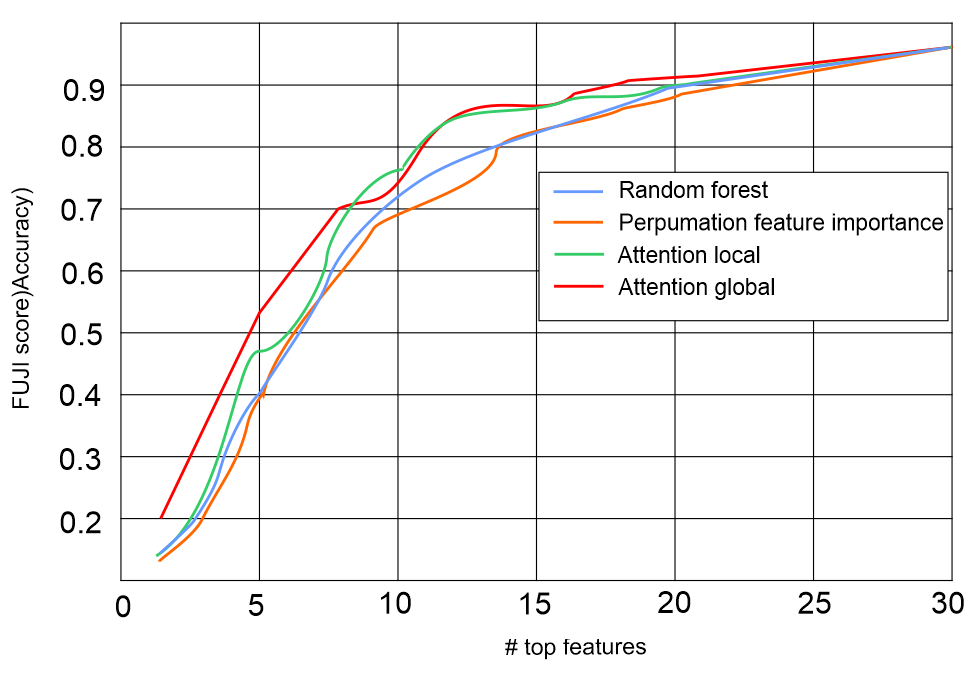
\includegraphics[scale=0.7]{images/fuji_score.png}
	\caption{FUJI score-based ranking comparison. The higher the FUJI score, higher the pairwise algorithmic similarity, when a certain number of features is considered.}
    \label{fig:fuji_score}
\end{figure*}

\begin{figure*}
	\centering
	\begin{subfigure}{.48\linewidth}
		\centering
		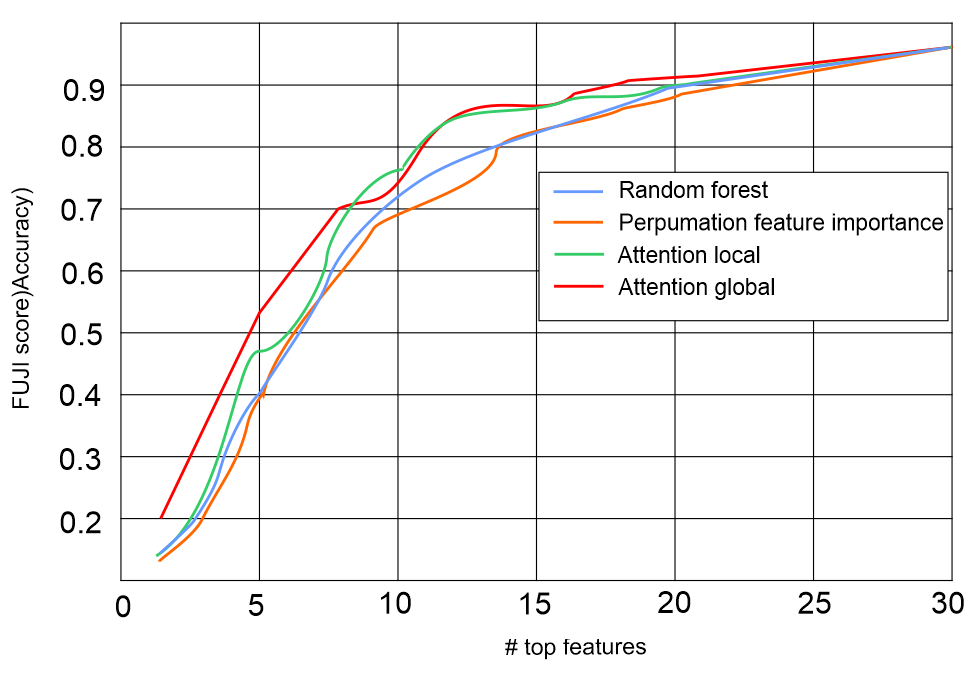
\includegraphics[scale=0.7]{images/fuji_score.png}
		\caption{FUJI score-based ranking comparison}
        \label{fig:fuji_score_compare}
	\end{subfigure}
	\hspace{2mm}
	\begin{subfigure}{0.48\linewidth}
		\centering
		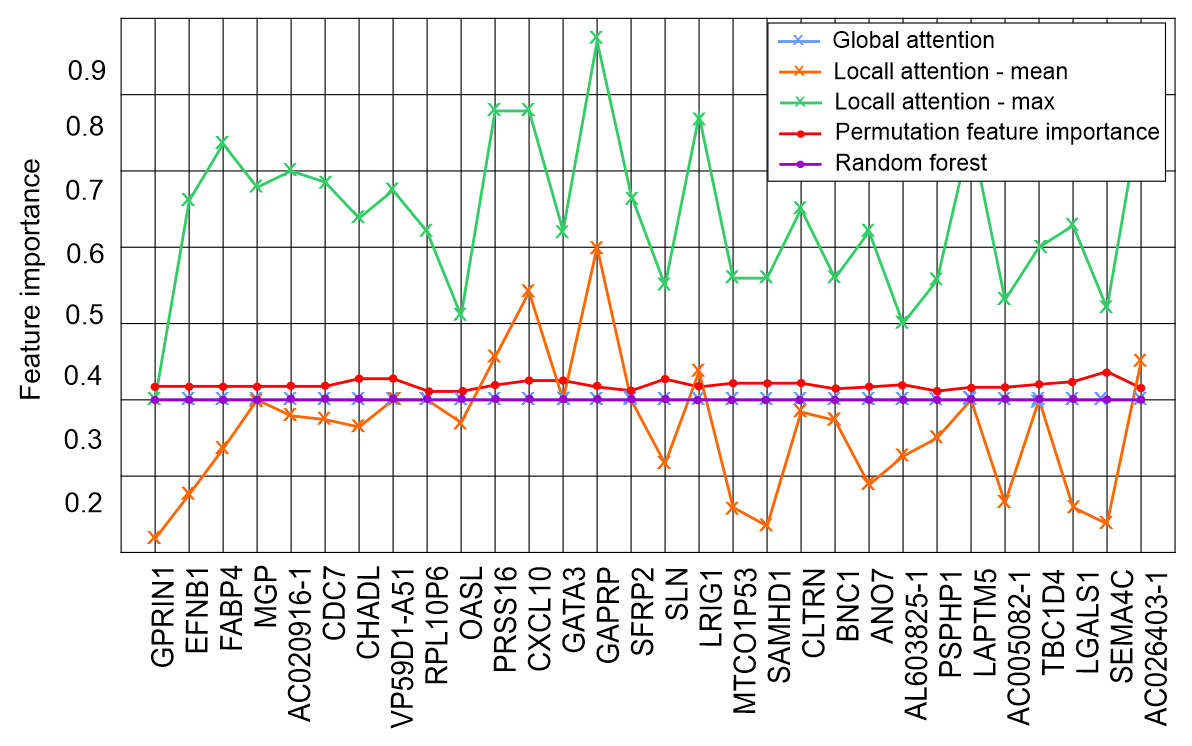
\includegraphics[scale=0.6]{images/am_fi_compare.png}
		\caption{Feature importance}
        \label{fig:relative_fi_am}
	\end{subfigure}
	\caption{a) The higher the FUJI score, higher the pairwise algorithmic similarity, when a certain number of features is considered, b) Relative feature importance for top-30 features} 
	\label{fig:comgenes}
\end{figure*}

In contrast, the proposed SANs exhibit a consistent mapping between the input space and the meaning of individual features, making possible the aggregation schemes considered in this work. In terms of general performance, this paper proves empirically that SANs can emit attention vectors that offer similar feature rankings
relevant for an external classifier (e.g., Logistic Regression). As the
purpose of this work was not excessive grid search across possible
architectures, which we leave for further work. Further, the proposed SANs
shall be compared to the recently introduced TabNet [2], an approach
that also attempts to unveil the feature importance landscape via sequential attention mechanism.

We next discuss the similarities between the considered feature importance approaches. The results are presented as FUJI curves, where we omit the space of all possible (pairwise) comparisons to the ones, that are compared with the proposed SANs. The results are shown in Figure 3. The considered visualizations depict at least two general patterns.

First, the attentionClean and attention-based importances are indeed very similar. We remind the reader that the difference between the two is that attentionClean only takes into account the correctly classified instances. Next, we can observe that ReliefF and Random Forestbased importances are different. Further, the global attention appears the most similar to Random Forest importances. Overall areas below
FUJI curves are shown in Figure 4. 6.3 Classification performance We next discuss the classification performance results. Let us remind the reader that the results show how the logistic regression (C = 1, L2 normalization) classifier performs when parts of the feature space are
pruned according to a given feature importance vector. The results
are shown in Figure 5.
The first observation—to our knowledge not known to the
community—is that SANs indeed perform competitively. Especially
on data sets with a large number of features, such as the p53, genes
and dlbcl (all biological ones), the attention mechanism detects larger
subsets of features that can improve the performance of the logistic
regression classifier, in e.g., dlbcl even outperforming all other approaches by a margin of more than 15%. On smaller data sets, SANs
perform competitively (e.g., madelon, optdigits, chess), or do not perform that well (biodeg-p2-discrete). Overall, worse performance of
SANs coincides with smaller data sets, indicating that not enough
data was present for SANs to distill the relevant parts of the feature
space. Further, it can be observed that ReliefF on data sets such as
pd-speech and madelon outperforms all other approaches, indicating
this state-of-the-art approach is suitable for low-resource situations

\subsection{Local explanations}
In order to explain individual diagnoses, only the important features w.r.t local feature impact is not enough. Sensitivity analysis in terms of what-if and leave-one-feature out analyses are found to be useful. 

\subsubsection{Local feature impacts}
Local feature impact identifies which features have the greatest positive or negative effect on the outcome of the $MCAE_{lrc}$ model for a specific row, i.e., individual sample. Features are most important in explaining the target variable, are shown on the top. As shown in \cref{fig:local_feature_impacts}, the average outcome predicted by the the $MCAE_{lrc}$ model is 9.758071. On average, variables TFAP2A, VPS9D1-AS1, and MTND2P28 will increase the average model outcome~(9.758071) by -0.36, 0.8, and 0.47, respectively. Variables TFAP2A, ADCY3, and FOXP4 will change the average model outcome by -0.36, -0.31, and-0.28, respectively. 

\begin{figure*}[h]
    \centering
	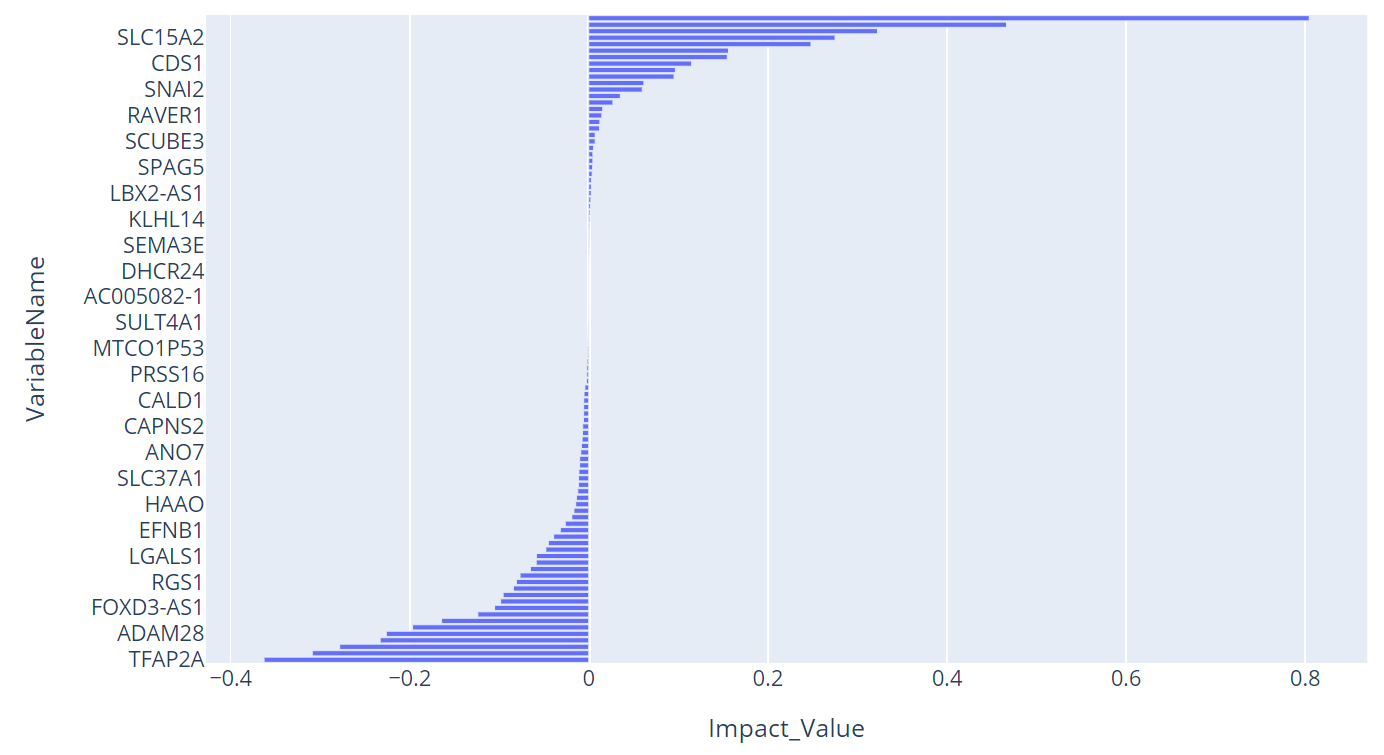
\includegraphics[scale=1.2]{images/local_fi_1.png}
	\caption[Local feature impact identifies which features have the greatest positive/negative effect]{Local feature impact identifies which features have the greatest positive or negative effect on the outcome of the $MCAE_{lrc}$ model for a specific row}
    \label{fig:local_feature_impacts}
\end{figure*}

\begin{figure*}[h]
    \centering
	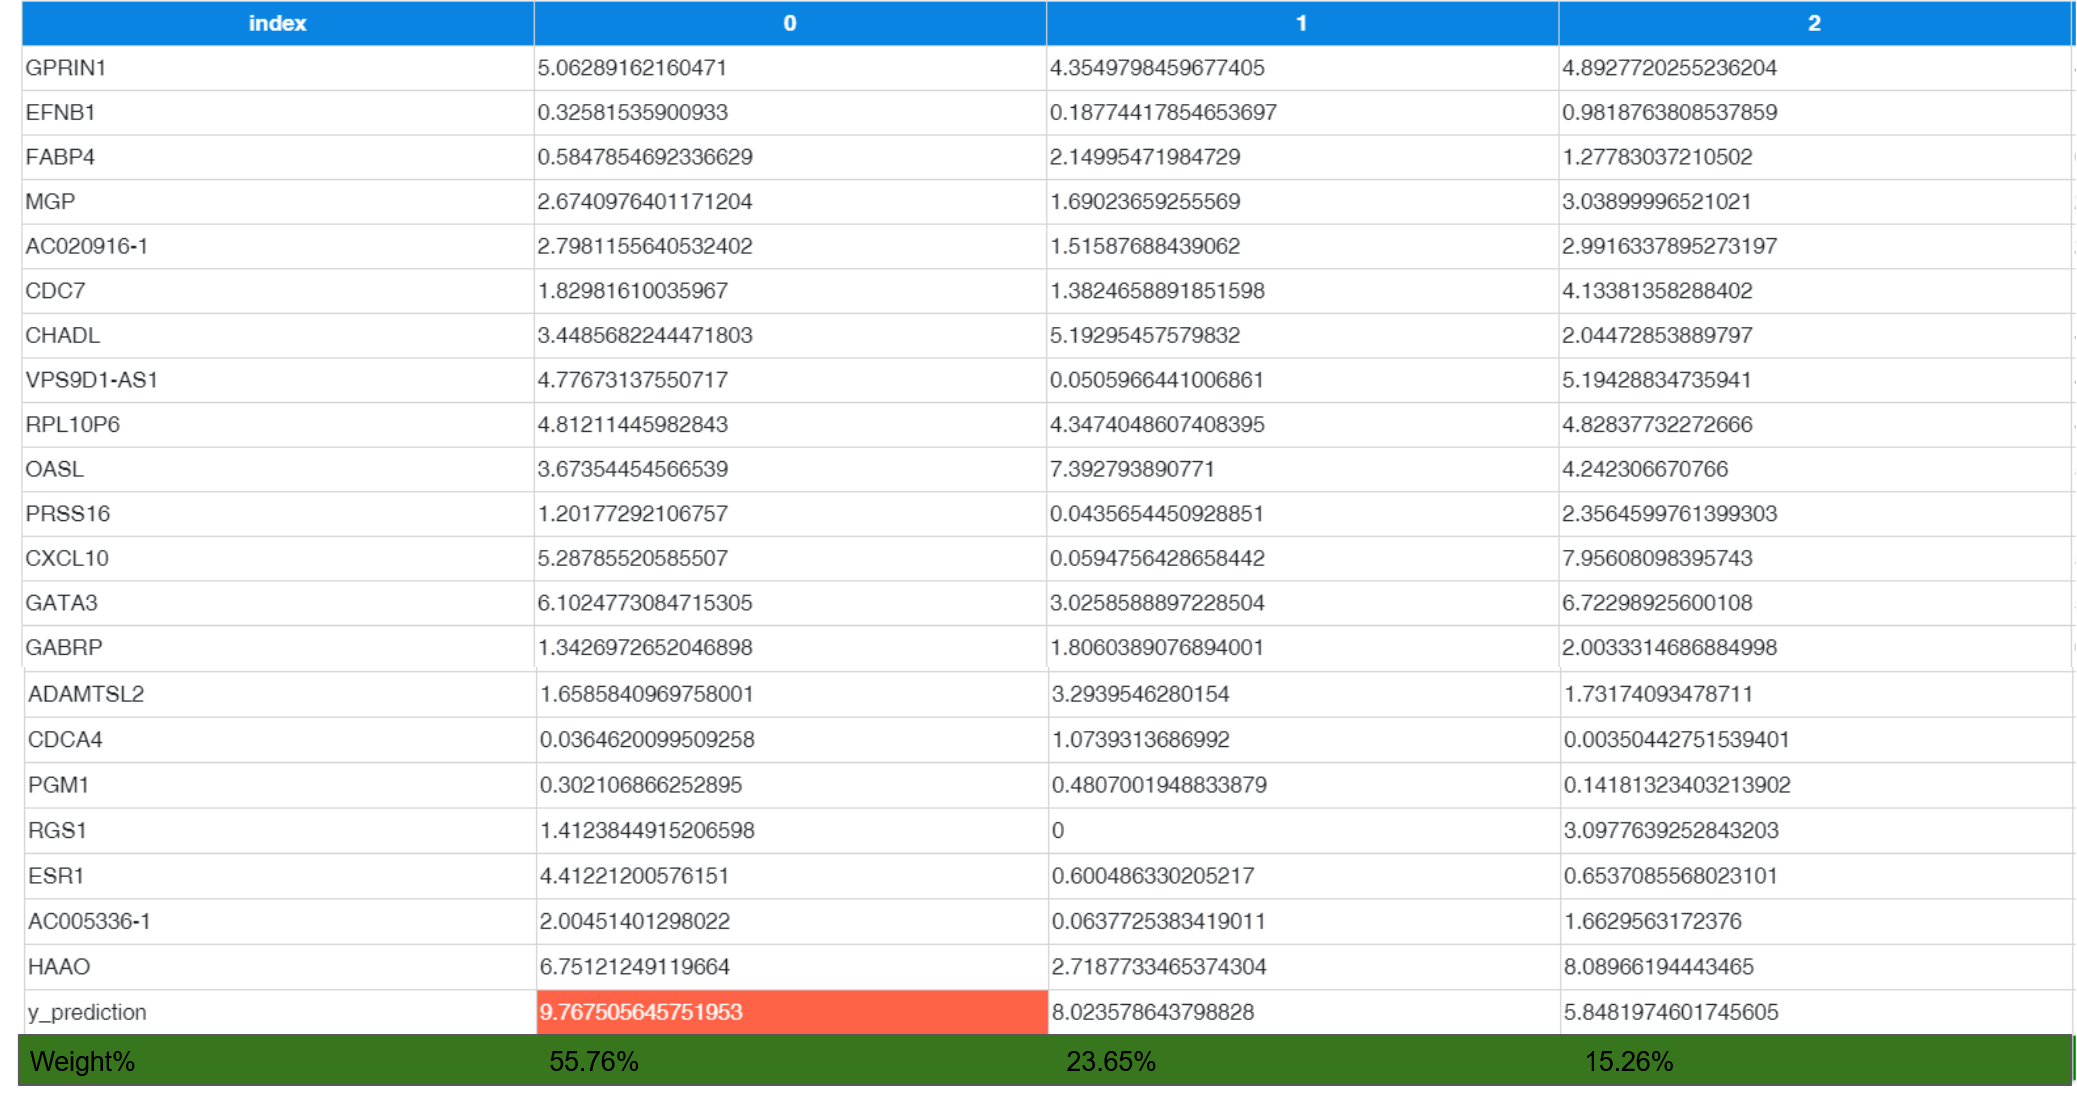
\includegraphics[scale=0.65]{images/similar_profiles.png}
	\caption{Similar patient cohorts identified by the $MCAE_{lrc}$ model}
    \label{fig:similar_patients}
\end{figure*}

%\hspace*{3.5mm} 

\hspace*{3.5mm} Further, to find which patients are similar to the patient being currently diagnosed are identified by computing the cosine similarity measure, as indicated by the last row in the table labelled as "Weight" in in \cref{fig:similar_patients}. This is a useful way of explaining to end users~(e.g., a patient or for doctor's understanding) that because Profile `A', Profile `B' and Profile `C' had very similar variables to specific row. Therefore, the model predicted a certain outcome. In this case, Profile 0 is 55.76\% similar, Profile 2 is 23.65\% similar, and Profile 4 is 15.26\% similar to the sample or row number 1 that we are trying to explain. Now the end user can comprehend how the model is making its decisions by looking at that patients.  

\subsubsection{Sensitivity analyses: what-if and leave-one-feature-out}
To quantitatively validate the feature-level relevances, what-if analysis is carried out. As shown in \cref{fig:what_if}, genes TFAP2A, VPS9D1-AS1, MTND2P28, ADCY3, FOXP4, GPRIN1, EFNB1, FABP4, MGP, AC020916-1, CDC7, CHADL, RPL10P6, OASL, and PRSS16 are most sensitive to making changes. On the other hand, making changes to SEMA4C, CWH43, HAGLROS, SEMA3E, and IVL does not have significant impact on the prediction. 

\begin{figure*}[h]
    \centering
	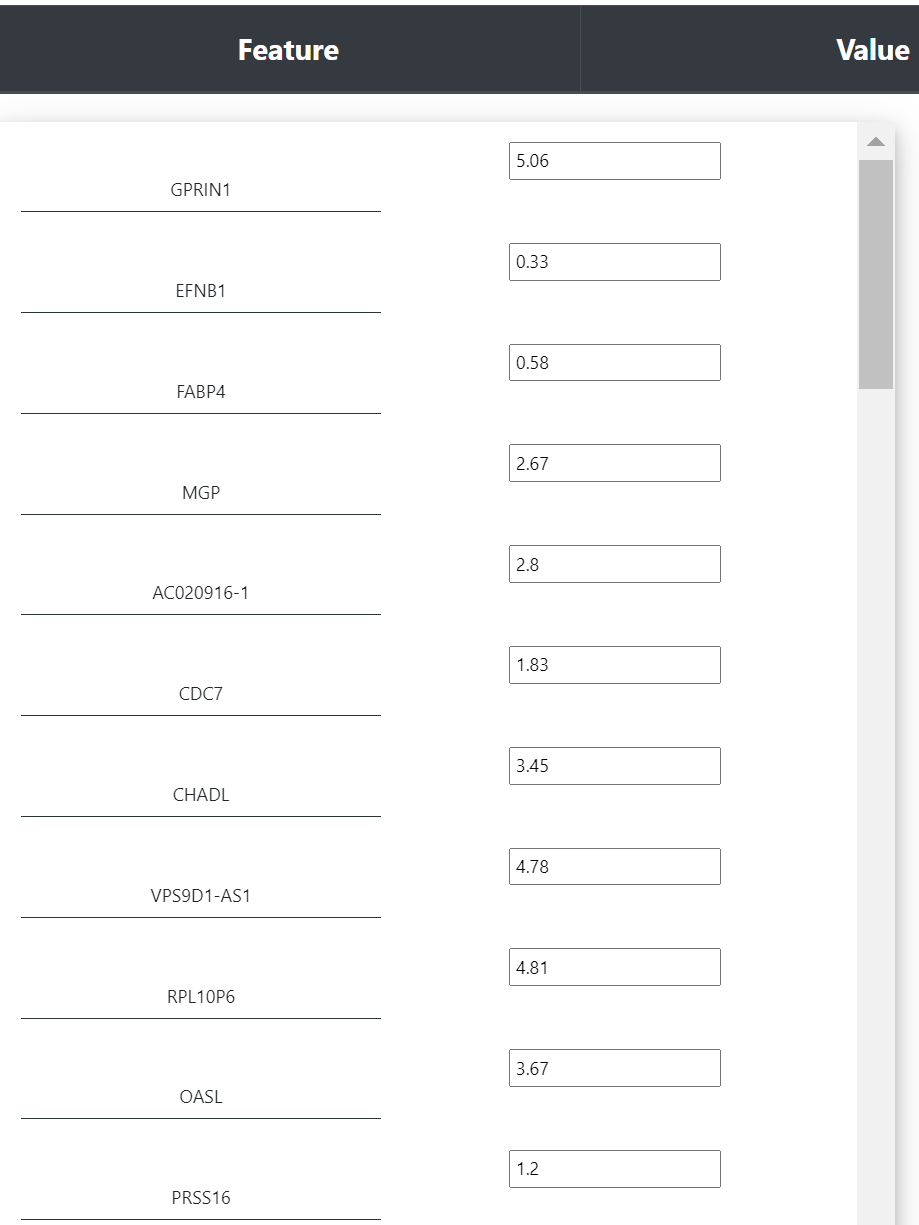
\includegraphics[scale=0.7]{images/what_if.png}
	\caption[What-if analysis]{What-if analysis, showing most important features for which making changes will impact the prediction most on the $MCAE_{lrc}$ model}
    \label{fig:what_if}
\end{figure*}

\subsubsection{Leave-one-feature-out analysis}
Display similar profiles and the extent to which they are similar to the chosen applicant as indicated by the last row in the table below labelled as "Weight". The idea is to improve the greedy backward elimination algorithm by preserving more interactions among terms. First, we randomly select a sample hate statement in test set. For the sample, we generate prediction probabilities for all the classes, followed by explaining word-level relevance for two highest probable classes. 

\begin{figure}[h]
    \vspace{-2mm}
	\centering
	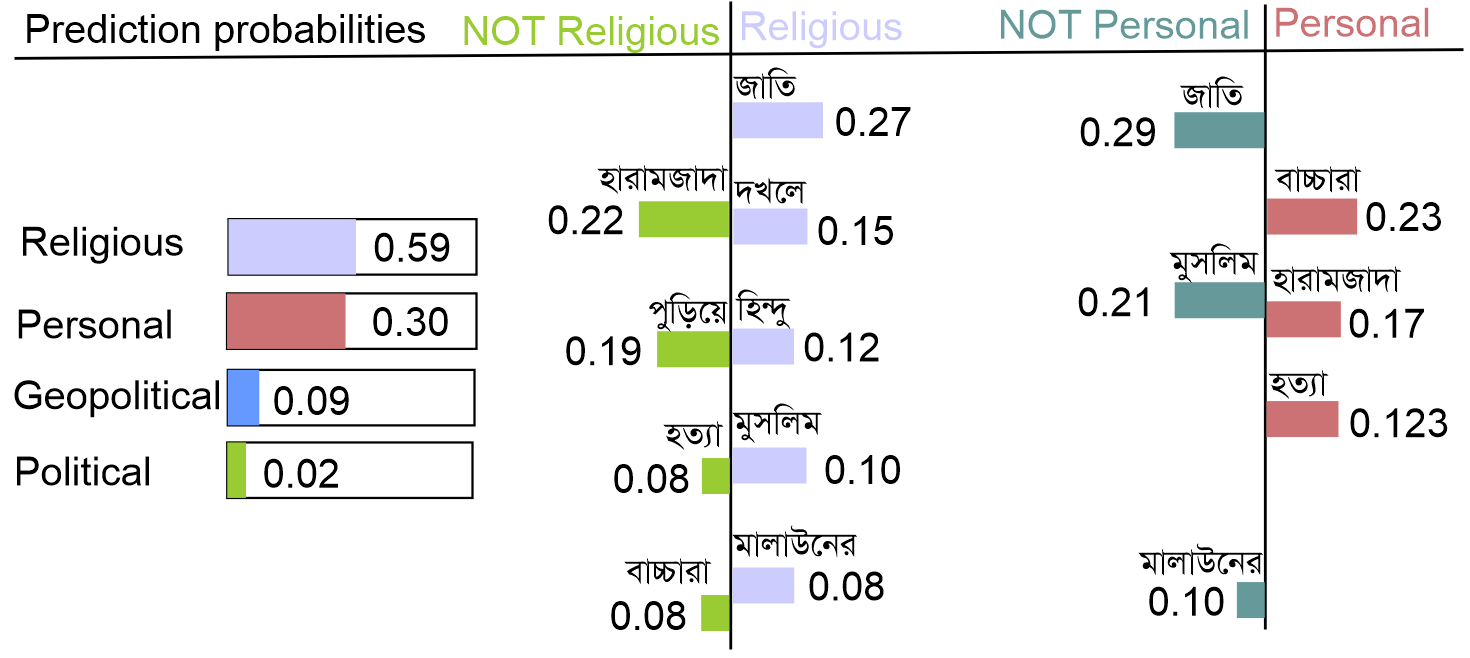
\includegraphics[scale=0.6]{images/reli_explain.png}
	\caption{Gene-level relevance test using leave-one-out test}
    \label{fig:explain_term_wise_religious_hate}
	\vspace{-4mm}
\end{figure}

\hspace*{3.5mm} First, we randomly pick a sample from the test set and perform the inferencing. Let's the model predicts the sample of COAD cancer types. As shown in \cref{fig:explain_term_wise_religious_hate}, features on the right side positively impacting the prediction, while features on the left are negatively. It turns out that features like TFAP2A,  VPS9D1-AS1, MTND2P28, ADCY3, nad FOXP4 are positive for COAD class, for this single inferencing. The feature TFAP2A has the highest positive score of 0.29 for class COAD. Our model predicts this as a COAD cancer type too, with the probability of 55\%. Besides, the sample could be of BRCA cancer type with a probability of 29\%.  

\hspace*{3.5mm} However, if we remove feature TFAP2A from the profile, we would expect the model to predict the label COAD with a probability of 26\%~(i.e., 55\% $-$ 29\%), making the actual prediction to be BRCA cancer type. On the contrary, features IVL, PRSS16, EFNB1, and CWH43 are more important features, having impacts of 0.23, 0.17, 0.123, and 0.07, respectively for the class BRCA. These features not only can reveal the relevance of important feature for classifier’s decision, but also signify that removing most relevant biomarkers will impact the prediction decision, accordingly to their relevance value. 

%\subsubsection{Similar profiles and summary plot}
%Display similar profiles and the extent to which they are similar to the chosen applicant as indicated by the last row in the table below labelled as "Weight".

\subsection{Measure of explainability}
For measuring the explainability, both unimodal and multimodal models are considered. However, since GE and miRNA modalities work well in multimodal setting, CNV modality is excluded from the calculation. Results of the faithfulness are shown in \cref{tab:faithfullness_result} in terms of comprehensiveness and sufficiency~(where the prefix is used to refer the DNN architecture, e.g., vanilla `CNN', `VGG16', `CAE', or `MCAE', and suffix refer to modality such as `g' for gene expression, `m' for miRNA, `c' for CNV.). As shown, unimodal $CNN_{m}$, $VGG16_{g}$, $VGG16_{m}$, $CAE_{g}$, and $CAE_{m}$ consistently outperforms $CNN_{g}$, $CNN_{g}$, $VGG16_{c}$, $CAE_{c}$, $MCAE_{lrc}$~(i.e., $f_1$), and $MCAE_{slr}$~(i.e., $f_2$) models. This signifies that a model which attain the best scores, %in terms of performance metrics, 
may not perform well in terms of faithfulness explainability metrics.  

\begin{table}[h]
    \centering
    \caption{Measure of explainability}
    \begin{tabular}{l|c|c}
        \hline \textbf{Classifier} & \textbf{Comprehensiveness} & \textbf{Sufficiency} \\ 
        \hline $CNN_{g}$ & 0.29 & 0.09 \\ \hline 
        $CNN_{m}$ & 0.21 & 0.05 \\
        \hline $CNN_{c}$ & 0.29 & 0.09 \\  
        \hline $VGG16_{g}$ & 0.29 & 0.09 \\ \hline 
        $VGG16_{m}$ & 0.21 & 0.05 \\
        \hline $VGG16_{c}$ & 0.29 & 0.09 \\ \hline 
        $MCAE_{lrc}$ & 0.21 & 0.05 \\
        \hline $MCAE_{slr}$ & 0.29 & 0.09 \\ 
        \hline
    \end{tabular}
    \label{tab:faithfullness_result}
\end{table}

\hspace*{3.5mm} Model $CNN_{g}$, $CNN_{c}$, $VGG16_{c}$, $CAE_{c}$ and $MCAE_{slr}$ have the worst score for sufficiency as compared to other models. Models $CAE_{g}$  $CAE_{m}$, and $MCAE_{lrc}$ turns out to be the best models for both sufficiency and comprehensiveness metric. Overall, $CAE_{g}$ performs the best among unimodal and $MCAE_{lrc}$ among multimodal model. As observed a model’s performance metric alone is not enough. Models with slightly lower performance, but much higher scores for faithfulness might be preferred for a sensitive and critical healthcare use cases such as cancer diagnosis at hand. 

\section{Chapter Summary}\label{chapter_5:conclusion}
In this chapter, two deep multimodal architectures called $MCAE_{lrc}$ and $MCAE_{slr}$ have been developed for cancer types prediction based on different combination of multimodal genomics data types. Besides, probing techniques such as GradCAM++, LRP, and attention mechanism employed on a vanilla CNN, an VGG16, $MCAE_{lrc}$, and $MCAE_{slr}$ networks. Experiment results show that omics data are useful useful for predicting cancer types with high confidence giving high f1 scores~(of up to 96.25\% for single modality based on GE and of up to 92.45\% for GE+miRNA input modalities). Based on this comparison, it would not be unreasonable to conclude that there is a possibility both $MCAE_{lrc}$ and $MCAE_{slr}$ might surpass MAE and ML baselines models such as GBT or RF performance with the right combination of inputs. 

\hspace*{3.5mm} The $MCAE_{lrc}$ model can predict cancer types 96.25\% of the cases correctly, which slightly outperforms the approach by Boyu et al.~\cite{lyu2018deep}, but 6.5\% better than the approach by Yuanyuan et al.~\cite{li2017comprehensive}. Further, $MCAE_{lrc}$ model reduces the false prediction rate for the READ, UCS, ESCA, and CHOL tumor samples. In particular, against 35\%, 81\%, 77\%, and 56\% of the correctly predicted cases by~\cite{lyu2018deep}, $MCAE_{lrc}$ can predict 88.74\%, 87.26\%, 89.56\%, and 84.55\% of the cases correctly. Although slightly underperforms than~\cite{lyu2018deep} at classifying BRCA, THCA, and PRAD~(in red), our $MCAE_{lrc}$ model is more consistent for the majority cancer types and likely to perform more stably on new GE data. Further, by we statistical analysis is provided to confirm if the identified genes are statistically relevant. Nevertheless, more human-interpretable explanations are shown, covering both global and local explanations of the diagnosis made, through a user-friendly interface. 

\hspace*{3.5mm} The downside is that several other factors have hindered this research too. For example, lack of enough training samples and single modality, i.e., only GE data used for making the predictions and generating the explanations. The latter reason caused the network to produce high training and validation errors during the training phase, giving lower accuracy during the inferencing phase. Although we attempted to open the CNN, VGG16, and MCAE `black-box' models through biomarker validation and feature ranking, our approach is mostly post-hoc as the explainability is based on test cases and results similar to LRP. Another potential limitation that during the writing of the dissertation, the usability survey was not performed. Consequently, SCS is not reported in the experiment result section. %Several further factors have hindered this research, such as lack of enough training samples, and lack of biological pathways analysis.
In a nutshell, this chapter disseminate the following findings and recommendations, based on experiments:  

\begin{enumerate}[noitemsep]
    \item \textbf{What types of machine learning model and neural network architectures are for suitable for handing multimodal inputs?} - traditional baselines ML models cannot handle multi-input types, hence not suitable for multimodality. 
    \item \textbf{What individual genomic modalities are more suitable for more accurate diagnosis?} experiments results show that GE and miRNA and their multimodality more reliable results for cancer subtype prediction. This also suggests that this input combination is suitable for multimodality integration for subsequent experiments. 
    \item \textbf{What multimodal input combinations are more suitable for more accurate diagnosis?} - experiments results show that GE + miRNA multimodality combination is more suitable for cancer subtype prediction. This also suggests that DNA methylation data is not suitable for cancer diagnosis, hence not suitable for multimodality integration for subsequent experiments.
    \item \textbf{What types of data can express biological characteristics of the patients?} - the qualitative analysis of the learned representation of GE + miRNA data can express biological characteristics of cohorts. Subsequently, the MAE learns latent molecular properties in coded form from patient expression profiles. This suggests that the hypothesis built upon is valid. 
    \item \textbf{How faithful the explanations are?} - based on comprehensiveness and sufficiency scores, it would not be unfair to claim this approach shows moderately high faithfulness w.r.t global explainability.   
    \item \textbf{What is more important: accuracy and explainability, or faithfulness?} Models with slightly lower performance, but much higher scores for plausibility and faithfulness might be preferred depending on the task at hand. 
\end{enumerate}

\hspace*{3.5mm} Now that the approach is sufficiently accurate, transparent, and explainable, in order to ensure an explainable model is robust to adversaries and behaves as intended in real-life treatment diagnosis, adversarial robustness of the model needs to be improved~\cite{bhatt2020explainable}. In the next chapter, different adversarial attacks will be introduced on our model, including content moderation, numeric data moderation, and out-of-distribution~(OOD), before assessing the robustness against each scenario. 
